\documentclass[12pt, oneside,a4paper]{article}
\usepackage[latin1]{inputenc}
\usepackage{TW_corp_ID}
%\definecolor{grau}{gray}{0.50}
\definecolor{grau2}{gray}{0.95}

\usepackage{bibgerm}
%\renewcommand\refname{TEST} funkt nicht?? title des literaturverzeichnisses zu �ndern!
\bibliographystyle{geralpha}


\usepackage{listings}
\renewcommand\lstlistingname{Listing}
\renewcommand\lstlistlistingname{Listings}
\lstdefinestyle{example} { %code listings: beispiele
		%language=Python,
    numbers=left, numberstyle=\scriptsize, stepnumber=1, numbersep=8pt,
    basicstyle=\ttfamily\footnotesize,
		backgroundcolor=\color{grau2},
		captionpos=b,
		showstringspaces=false,
		tabsize=4
		%commentstyle=\color{blue},%  Kommentar blau
		%keywordstyle=\color{red},%   Schl�sselw�rter rot
		%stringstyle=\color{green} % typewriter type for strings
}
\lstdefinestyle{interpreter} {%inline interpreter beispiele
		numbers=none,
		tabsize=4,
		basicstyle=\ttfamily\footnotesize,
		moredelim=[l][{\bfseries}]{>>>},
		moredelim=[l][{\bfseries}]{...}
}

% sollte als letztes Packet geladen werden (wenn glossary nicht verwendet wird ;) )
\usepackage{hyperref} 

%glossar. um die verlinkung durch hyperref zu garantieren, muss dieses packet NACH hyperref geladen werden.
\usepackage[
style=super,
%hypertoc=true, %erscheint im inhaltsverzeichnis
hyper=true, % eintr�ge verlinken
number=none, % keine pagerefs
header=none,
acronym=true %dieser Parameter ist der wichtige
]{glossary}
\setacronymnamefmt{\gloshort} %um das abk�rzungsverzeichnis korrekt zu formatieren
\renewcommand{\acronymname}{Verwendete Abk�rzungen}
%\makeglossary
\makeacronym

\begin{document}
\pagestyle{TWcorpID}
\newacronym{Zope}
{Z Object Publishing Environment}
{description=Z Object Publishing Environment}

\newacronym{ZPL}
{Zope Public Licence}
{description=Zope Public Licence}

\newacronym{BSD}
{Berkeley Software Distribution}
{description=Berkeley Software Distribution}

\newacronym{PSF}
{Python Software Foundation}
{description=Python Software Foundation}

\newacronym{PSA}
{Python Software Activity}
{description=Python Software Activity}

\newacronym{SIG}
{Special Interest Group}
{description=Python Special Interest Group}
 
\newacronym{CI}
{Corporate Identity}
{description=Corporate Identity}  

\newacronym{NASA}
{National Aeronautics and Space Administration}
{description=National Aeronautics and Space Administration}  
 
\newacronym{CWI}
{Centrum voor Wiskunde en Informatica}
{description=Centrum voor Wiskunde en Informatica}   
 
\newacronym{ZODB}
{Zope Object Database}
{description=Zope Object Database}     
  
\newacronym{ORB}
{Object Request Broker}
{description=Object Request Broker}        

\newacronym{CPS}
{Collaborative Portal Server}
{description=Collaborative Portal Server}        

\newacronym{ZCML}
{Zope Configuration Markup Language}
{description=Zope Configuration Markup Language}        

\newacronym{XML}
{Extensible Markup Language}
{description=Extensible Markup Language}        

\newacronym{WWF}
{World Wide Fund For Nature}
{description=World Wide Fund For Nature}        

\newacronym{NATO}
{North Atlantic Treaty Organisation}
{description=North Atlantic Treaty Organisation}        

\newacronym{DTML}
{Document Template Markup Language}
{description=Document Template Markup Language}        

\newacronym{ZPT}
{Zope Page Templates}
{description=Zope Page Templates}

\newacronym{TTW}
{Through the Web}
{description=Through the Web}        

\newacronym{URL}
{Uniform Resource Locator}
{description=Uniform Resource Locator}

\newacronym{HLL}
{High Level Language}
{description=High Level Language}

\newacronym{SQL}
{Structured Query Language}
{description=Structured Query Language}

\newacronym{RDBMS}
{Relational Database Management System}
{description=Relational Database Management System}

\newacronym{HTML}
{Hypertext Markup Language}
{description=Hypertext Markup Language}

\newacronym{CSS}
{Cascading Style Sheets}
{description=Cascading Style Sheets}

\newacronym{PDF}
{Portable Document Format}
{description=Portable Document Format}

\newacronym{PROLOG}
{PROgramming in LOGic}
{description=PROgramming in LOGic}

\newacronym{DBC}
{Design by Contract}
{description=Design By Contract}

\newacronym{AOP}
{Aspektorientierte Programmierung}
{description=Aspektorientierte Programmierung}

\newacronym{UML}
{Unified Modeling Language}
{description=Unified Modeling Language}

\newacronym{OOP}
{Objektorientierte Programmierung}
{description=Objektorientierte Programmierung}

\newacronym{APE}
{Adaptable Persistence Engine}
{description=Adaptable Persistence Engine}

\newacronym{ZEO}
{Zope Enterprise Objects}
{description=Zope Enterprise Objects}

\newacronym{AJAX}
{Asynchronous JavaScript and XML}
{description=Asynchronous JavaScript and XML}

\newacronym{RSS}
{Really Simple Syndication}
{description=Really Simple Syndication}

\newacronym{FH}
{Fachhochschule}
{description=Fachhochschule}

\newacronym{IDLE}
{Integrated Development Environment}
{description=Integrated Development Environment}

\newacronym{GNU}
{GNU's Not Unix}
{description=GNU's Not Unix}

\newacronym{GUI}
{Graphical User Interface}
{description=Graphical User Interface}

\newacronym{Tcl}
{Tool command language}
{description=Tool command language}

\newacronym{Tk}
{Toolkit}
{description=Toolkit}

\newacronym{SDL}
{Simple DirectMedia Layer}
{description=Simple DirectMedia Layer}

\newacronym{API}
{Application Programming Interface}
{description=Application Programming Interface}

\newacronym{XP}
{Extreme Programming}
{description=Extreme Programming}

\newacronym{TDD}
{Test Driven Development}
{description=Test Driven Development}

\newacronym{HTTP}
{Hypertext Transfer Protocol}
{description=Hypertext Transfer Protocol}

\newacronym{CBSE}
{Component Based Software Engineering}
{description=Component Based Software Engineering}

\newacronym{COTS}
{Commercial Off-The-Shelf}
{description=Commercial off-the-shelf}

\newacronym{EJB}
{Enterprise Java Beans}
{description=Enterprise Java Beans}

\newacronym{RMI}
{Remote Method Invocation}
{description=Remote Method Invocation}

\newacronym{CORBA}
{Common Object Request Broker Architecture}
{description=Common Object Request Broker Architecture}

\newacronym{SOAP}
{Simple Object Access Protocol}
{description=Simple Object Access Protocol}

\newacronym{RPC}
{Remote Procedure Call}
{description=Remote Procedure Calls}

\newacronym{ZMI}
{Zope Management Interface}
{description=Zope Management Interface}

\newacronym{MUW}
{Medizinische Universit�t Wien}
{description=Medizinische Universit�t Wien}












\Diplom{$\ll$Python und Zope als Unterrichtswerkzeuge$\gg$}{Dominique Lederer}{Strassergasse 8-12/2/3\newline1190 Wien}{Dipl.-Ing. Dr. Karl M. G�schka}{Dipl.-Ing. (FH) Alexander Weiss}{Wien}{30.5.2007}{Informations- und Kommunikationssysteme}

\pagenumbering{Roman}

F�r Anf�nger ist das Erlernen einer Programmiersprache schwierig. Das liegt daran, dass im heutigen Unterricht bevorzugt mit Sprachen aus der Industrie gelehrt wird. Studenten wollen in der Industrie Jobs bekommen, und legen deshalb Wert darauf, dass gefragte Technologien Bestandteil ihrer Ausbildung sind. Die Industrie wiederum will ihren Bedarf befriedigen. Dabei wird �bersehen, dass Programmiersprachen keine Technologien selbst, sondern Werkzeuge f�r Technologien sind. Im Unterricht muss eine Programmiersprache ein Werkzeug sein, mit dessen Hilfe es m�glich ist, die fundamentalen Ideen eines Unterrichtsgegenstandes zu vermitteln, ohne in einen Unterricht �ber die Programmiersprache selbst abzudriften.

Die vorliegende Arbeit stellt Python als ein solches Werkzeug vor. Sie zeigt auf, dass Python, im Gegensatz zu heute h�ufig im Unterricht zum Einsatz kommenden Sprachen (wie C, C++ oder Java), gut f�r Anf�nger geeignet ist. Aufgrund des einfachen Zugangs k�nnen mit Python viel fr�her relevante Konzepte der Informatik und Softwareentwicklung diskutiert werden. Ein weiterer wesentlicher Vorteil ist, dass auch die Arbeit der Unterrichtenden erleichtert wird. Die Sprache ist kompakt und simpel gehalten und versucht sich dem Entwickler nicht in den Weg zu stellen. Gleichzeitig ist sie eine allgemein anerkannte Sprache und findet Verwendung in der Industrie.


\newpage
%\section*{Verwendete Abk�rzungen}
\rkopf[]{Verwendete Abk�rzungen}
\printacronym 

%\printglossary 
%\glossary{
%name=Individualsoftware,
%description={Individualsoftware zeichnet sich dadurch aus, dass sie nur f�r einen oder f�r wenige Anwendungsf�lle geschaffen wird.}
%}

\newpage
\section*{Eidesstattliche Erkl�rung}
\rkopf[]{Eidesstattliche Erkl�rung}
"'Ich erkl�re hiermit an Eides statt, dass ich die vorliegende Arbeit selbst�ndig angefertigt habe. Die aus fremden Quellen direkt oder indirekt �bernommenen Gedanken sind als solche kenntlich gemacht. Die Arbeit wurde bisher weder in gleicher noch in �hnlicher Form einer anderen Pr�fungsbeh�rde vorgelegt und auch noch nicht ver�ffentlicht."'\vspace{1cm}\\

\newpage
\pagenumbering{arabic}
\rkopf[]{Inhaltsverzeichnis}

\tableofcontents
\newpage

%%%
\section{Einleitung}
\rkopf[]{Einleitung}

%TODO Vor Fertigstellung\footnote{Wenn in dieser Arbeit die m�nnliche Form verwendet wird, sind Frauen gleicherma�en gemeint, sofern nichtexplizit Gegenteiliges behauptet wird.} der Arbeit diese Fu�note an geeigneter Stelle anbringen.

	\subsection{Motivation und Zielsetzung}
		%Was will diese Arbeit? Warum wird sie geschrieben? Was ist das Ziel? Was ist der Mehrwert?
%Thema? Ziel?

Geht es um das Aneignen von Programmierkenntnissen, ist die momentane Situation nach Ansicht des Autors nicht optimal.
Sie ist verbesserungsw�rdig. Gerade in der schnelllebigen Informatik sollte im Unterricht nicht auf Trends oder Modeerscheinungen zur�ckgegriffen werden, sondern die fundamentalen Ideen der Wissenschaft Informatik mit einem guten Konzept an die Studierenden herangetragen werden. Erste Programmierkenntnisse mit z.B. C oder Java zu vermitteln bzw. vermittelt zu bekommen, ist problematisch. Diese Arbeit hat zum Ziel, einen einfacheren Weg aufzeigen und soll begr�nden, warum erste Programmiererfahrungen mit Python didaktisch sinnvoller sind.

Die Programmiersprache Python soll als Programmiersprache f�r den Unterrichtseinsatz vorgestellt werden und es wird gezeigt, wie gewisse Grundkonzepte mittels dieses Werkzeugs vermittelt werden k�nnen. Weiterf�hrend wird \Zope\ als Applikationsserver, basierend auf Python, f�r fortgeschrittenere Themen der Softwareentwicklung, und vor allem f�r den praktischen Teil dieser Arbeit verwendet.

Die Arbeit hat das Ziel, die Verbreitung von Python an Schulen und Universit�ten zu unterst�tzen, um damit den Sch�lern\footnote{Wenn in dieser Arbeit die m�nnliche Form verwendet wird, sind Frauen gleicherma�en gemeint, sofern nicht explizit Gegenteiliges behauptet wird.} und Studenten den Einstieg in die Programmierung und diese selbst zu erleichtern. 

Weiters ist \Zope\ f�r den Einsatz an Universit�ten vorzustellen; der einfache Zugang zu einem Open-Source Produkt soll die Vorteile f�r Lektoren und Studenten bei fortgeschrittenen Themen der Softwareentwicklung aufzeigen.

Die vorliegende Arbeit soll dabei als Entscheidungs- und Argumentationsgrundlage an genannten Ausbildungseinrichtungen dienen k�nnen.

%It has always been Van Rossum's desire to see Python used for teaching, 
 




	\subsection{Aufbau der Arbeit}
		Die Arbeit gliedert sich in Einleitung, zwei Hauptkapitel und abschlie�ende Diskussion. Sie ist nicht klassisch in Theorie- und Praxisteil gegliedert. Eine solche Aufteilung ist bei dieser Thematik schwer zu vollziehen, die vorgestellte Theorie wird immer wieder durch praktische Beispiele unterst�tzend erl�utert. Im zweiten Kapitel ist eine Beispielimplementierung abgehandelt.

In der Einleitung werden die Argumentationsgrundlagen f�r die Arbeit aufgebaut. Die in der Arbeit verwendeten Technologien Python und \Zope\ werden vorgestellt. 

Nach Erkl�rung allgemeiner, in der Arbeit verwendeter Begrifflichkeiten und Technologien, folgt im ersten Kapitel die Abhandlung der Programmiersprache Python. Darin wird erl�utert, warum sich Python als eine Einstiegsprogrammiersprache, und vor allem f�r Unterrichtszwecke besonders gut eignet. Danach werden Grundkonzepte des Informatikunterrichts, wie Paradigmen und Algorithmen mit Python als unterst�tzendes Werkzeug analysiert. Weiters wird behandelt, welche andere Fachgegenst�nde neben Informatik von Python profitieren k�nnen, wie das Thema Open-Source auf den Unterricht angewandt werden kann, und welche Materialien und Werkzeuge als Unterst�tzung f�r den Unterricht bzw. die Unterrichtsgestaltung zur Zeit zur Verf�gung stehen.

\Zope\ ist das Thema des zweiten Kapitels. \Zope\ ist ein Applikationsframework basierend auf Python und eignet sich f�r das Lehren fortgeschrittener Softwareentwicklungsmethoden. Darin wird untersucht, ob \Zope\ als Komponentensystem betrachtet werden kann, und wie das Framework mit \CBSE\ in Verbindung gebracht werden kann. Dass das Testen und Dokumentieren von Software im Unterricht vernachl�ssigt wird, wird ebenso behandelt, wie das Lehren eines Softwareentwicklungsprozesses. Den Abschlu� des Hauptteils bildet die Beispielimplementierung aus einem realen Projekt im Arbeitsumfeld des Autors.
	
  \subsection{Fundamentale Ideen als Unterrichtsprinzip}
  	%Einleitende Worte zum Thema "Didaktisches Prinzip".\cite{bruner}
Eine Argumentationsgrundlage dieser Arbeit ist die Definition einer \emph{fundamentalen Idee} nach Schwill \cite{schwill1}. In seiner Arbeit untersucht er die philosophische Sicht der \emph{Idee} nach Plato und Kant, und formuliert diese mit den \emph{Strukturen} nach J.S. Bruner \cite{bruner} zur fundamentalen Idee. J.S. Bruner hat das didaktische Prinzip an den Strukturen der zugrundeliegenden Wissenschaft, an denen sich der Unterricht orientieren soll, formuliert.

\begin{quote}   
{\itshape "'Eine \textbf{fundamentale Idee} (bezgl. einer Wissenschaft) ist ein Denk-, Handlungs-, Beschreibungs- oder Erkl�rungsschema, das
\begin{enumerate}
	\item in verschiedenen Bereichen (der Wissenschaft) vielf�ltig anwendbar oder erkennbar ist (Horizontalkriterium),
	\item auf jedem intellektuellen Niveau aufgezeigt und vermittelt werden kann (Vertikalkriterium),
  \item in der historischen Entwicklung (der Wissenschaft) deutlich wahrnehmbar ist und l�ngerfristig relevant bleibt (Zeitkriterium),
  \item einen Bezug zu Sprache und Denken des Alltags und der Lebenswelt besitzt (Sinnkriterium)."'
\end{enumerate}}
\end{quote}

\begin{figure}[h]
	\centering
	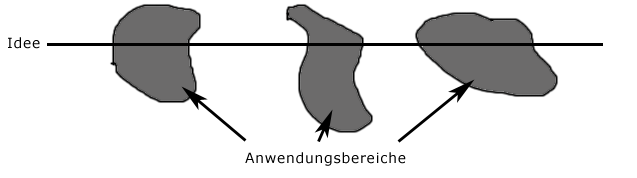
\includegraphics[scale=0.6]{graphics/horizontalkriterium.png}
	\caption{Horizontalkriterium nach \cite{schwill1}}
	\label{fig:horizontalkriterium}
\end{figure}

Das \emph{Horizontalkriterium} veranschaulicht Schwill wie in Abbildung \ref{fig:horizontalkriterium}. Eine Idee wird soweit abstrahiert, dass fachspezifische Elemente herausfallen. Damit kann themen- und fach�bergreifend gearbeitet werden. Der Lernende erkennt durch immer wiederkehrende Prinzipien die �bergreifende Relevanz der Thematik. Anschlie�end wird durch Wiederholung das Wichtige gefestigt. Die gemeinsame Idee kann jedoch wiederum nur durch umfassendes Spezialwissen herausgearbeitet werden. Das ist die Aufgabe der Lehrkr�fte.

Das \emph{Vertikalkriterium} kann wie ein Faden im Bildungsweg gesehen werden. Diesem Faden wird im Laufe der Ausbildung gefolgt. Dabei steigen das Niveau und die Detaillierung der Materie (Abbildung \ref{fig:vertikalkriterium}).

\begin{figure}[h]
	\centering
	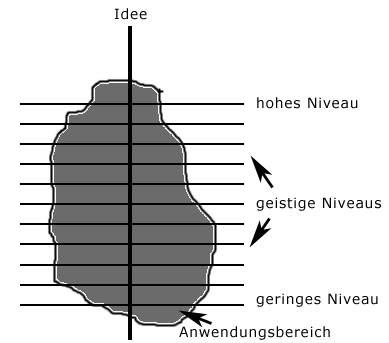
\includegraphics[scale=0.6]{graphics/vertikalkriterium.png}
	\caption{Vertikalkriterium nach \cite{schwill1}}
	\label{fig:vertikalkriterium}
\end{figure}

Das \emph{Zeitkriterium} ist in der Informatik nicht schwer zu erf�llen. Die Schnelllebigkeit der Technik birgt zwar viele Modeerscheinungen, jedoch sichert das Kriterium die Kontinuit�t des Unterrichts und den Wert der Kenntnisse und Erfahrungen der Unterrichtenden und verhindert fachliche Moden.\cite{misc:Modrow}

%\begin{quote}   
%{\itshape "'Das Kriterium sichert die Kontinuit�t des Unterrichts und den Wert der Kenntnisse und Erfahrungen der %Unterrichtenden und verhindert fachliche Moden."'}\cite{misc:Modrow}
%\end{quote}

Dabei ist die Tr�gheit der Lehre eine Art Vorauslese, um das Zeitkriterium einer fundamentalen Idee zu erf�llen.

Der Autor interpretiert das \emph{Sinnkriterium} als das tats�chliche Wertempfinden beim Empf�nger der Idee, beim Lernenden. Wie gut kann die Thematik als praxisrelevant oder als sinnvoll erkannt werden? Kann der Bezug zur sp�teren Verwendung in der Arbeitswelt hergestellt werden?

Der Einsatz fundamentaler Ideen wird von \cite{misc:Modrow} wie folgt beschrieben:

\begin{quote}   
{\itshape "'Der Unterricht muss dann so angelegt werden, dass sich diese - wenigen - fundamentalen Ideen bei den Sch�lerinnen und Sch�lern bilden k�nnen, er muss Kenntnisse und Erfahrungen vermitteln, die anhand dieser Ideen zu ordnen sind, und er muss diese Ideen zu einem geeigneten Zeitpunkt explizit thematisieren, um die spezifischen M�glichkeiten und Beschr�nkungen der Informatik in Abgrenzung gegen andere Disziplinen erkennbar zu machen."'}
\end{quote}

Einige Beispiele fundamentaler Ideen und die dazugeh�rigen Kriterien sind in \cite{schwill2} zu finden.
  
  %\subsection{Informatik im Unterricht}
  %Status quo der gelehrten Inhalte bezugnehmend auf \cite{schwill1}. Abgrenzung spezifischer und nicht-spezifischer Wissenstransfer. 
  
  %"Die Studenten stehen ratlos vor einer Unmenge von Einzelheiten, die weder zu gro�en Ideen noch zu allt�glichem Denken eine Beziehung erkennen lassen."

	\subsection{Programmiersprachen im Unterricht}
		\label{kapitel:Programmiersprachen}
		Ein vieldiskutiertes Thema ist, welche Sprache sich f�r den Unterricht am besten eignet. \cite{python:CRPITV52P71-80, misc:palumbo} meint, dass der Lernerfolg von der Zeit abh�ngt, die f�r tats�chliches Programmieren aufgewendet werden kann. Es sollte keine Zeit mit sprachspezifischen Eigenheiten und Syntaxproblemen "'verschwendet"' werden. Geht es nach \cite{python:CRPITV52P71-80, misc:milbrandt}, hat eine Programmiersprache f�r Unterrichtszwecke einen einfachen Zugang. Sie sollte leicht erlernbar sein, eine klare Struktur haben und vielf�ltig einsetzbar sein. Die Sprache hat eine einfache Syntax, einfaches I/O Handling, verst�ndliche String-Manipulation, aussagekr�ftige Schl�sselw�rter und verst�ndliches Feedback im Fehlerfall.

W�hrend Pascal und Logo vor einigen Jahren noch oft im Unterricht zum Einsatz kamen, sind beide heute stark aus der Mode gekommen. Gr�nde daf�r sind sicher die mangelnde Einsatzf�higkeit in der Industrie und die, so gut wie nicht m�gliche, Verwendbarkeit der Sprache bei steigender Komplexit�t der Software.

Heute z�hlen Sprachen wie C, Java und C++ zu den beliebtesten Programmiersprachen. Das ist an der Anzahl der verf�gbaren Entwickler, Lehrg�nge und Dienstleister weltweit zu erkennen \cite{misc:TIOBE}. Studien wie \cite{misc:deRaadt}, \cite{python:industry2} und \cite{misc:stephenson} belegen, dass Java, C++ und C die Sprachen mit der gr��ten Verbreitung an Universit�ten sind.

Trotz dieser Beliebtheit (oder gerade deswegen) wird viel �ber die Tauglichkeit dieser Sprachen im Unterricht diskutiert, gerade wenn es um geeignete Sprachen f�r Programmieranf�nger geht. Die oben genannten Sprachen werden als �berladen betrachtet. Die Studierenden plagen sich eher mit der Notation, als mit dem tats�chlichen Algorithmen. \cite{python:CRPITV52P71-80} erl�utert, dass die meisten Probleme von Programmierneulingen immer dasselbe Muster zeigen:
\begin{quote}
{\itshape "'[...] construct-based problems, which make it difficult to learn the correct semantics of language constructs, and plan composition problems, which make it difficult to put plans together correctly [...] students lack the skills needed to trace the execution of short pieces of code after taken their first course on programming."'}
\end{quote}

Im Zuge einer Studie an der finnischen Universit�t in Tampere ist eine Umfrage an europ�ischen Hochschulen durchgef�hrt worden. 559 Studenten und 34 Lektoren an 6 verschiedenen Universit�ten wurden unter anderem zu deren Schwierigkeiten beim Lernen und Lehren von Programmiersprachen befragt. Die daraus abgeleiteten Folgerungen besagen:
\begin{quote}
{\itshape "'the most difficult concepts to learn are the ones that require
understanding larger entities of the program instead of just details [...] abstract concepts like pointers and memory handling are difficult
to learn [...] However, the biggest problem of novice programmers does not seem to be the understanding of basic concepts but rather learning
to apply them."'}\cite{misc:difficulties}
\end{quote}

Die Studenten haben Probleme, wenn es darum geht, den Gesamtumfang eines Programmes zu erfassen und umzusetzen, dh. wie setze ich eine mir gestellte Aufgabe mit den Konzepten um, die ich gelernt habe. Dabei darf die Syntax einer Sprache nicht im Wege stehen, da sie daran hindert eine Probleml�sung zu finden und nur neue, andere Probleme schafft. Zeiger und Speichermanipulation z�hlen zu den als sehr schwierig eingestuften Konzepten.

Die in diesem Kapitel zitierte Literatur deckt sich mit den Beobachtungen des Autors aus der eigenen Ausbildung und der Abhaltung eines C Tutoriums f�r Programmieranf�nger. Die Studenten konnten genau wiedergeben, wie sie das Problem l�sen w�rden, doch konnten sie es nicht "'zu Papier"' bringen, also als Quelltext wiedergeben. Die Syntax wurde als unnat�rlich und teilweise unverst�ndlich empfunden. Manche syntaktische Eigenheiten sind f�r den Tutor auch schwer zu erkl�ren, da die Studenten die dahinterliegenden Konzepte noch nicht verstehen k�nnen. Nahezu alle Fehler resultierten aus einem Fehler in der Syntax. Der Autor konnte dabei ein hohes Ma� an Frustration und Demotivation der Studenten im Unterricht feststellen. Die Sinnhaftigkeit des Lehrinhaltes wurde weiters angezweifelt.
	
	\subsection{Grundlagen Python}						
		%\subsubsection{Was ist Python}
			\label{kapitel:Was_ist_Python}
			%Python is an interpreted, interactive, object-oriented programming language. It incorporates modules, exceptions, dynamic typing, very high level dynamic data types, and classes. Python combines remarkable power with very clear syntax. It has interfaces to many system calls and libraries, as well as to various window systems, and is extensible in C or C++. It is also usable as an extension language for applications that need a programmable interface. Finally, Python is portable: it runs on many Unix variants, on the Mac, and on PCs under MS-DOS, Windows, Windows NT, and OS/2.
Python ist eine dynamische "`High-Level"' Programmiersprache, die den interpretierten Skriptsprachen zugeordnet und oft mit Perl, Ruby, Scheme oder Java verglichen wird. Sie wurde mit dem Ziel entwickelt, m�glichst einfach und �bersichtlich zu sein, gleichzeitig aber nicht an Flexibilit�t und funktionaler Skalierbarkeit einb��en zu m�ssen.

Die Syntax ist sehr �bersichtlich gehalten, was unter anderem durch zwingende Einr�ckung des Quelltextes erreicht wird (siehe Listing \ref{python:syntax}). Grammatikalisch ist auf wenige Schl�sselw�rter optimiert worden\footnote{Mit Python 2.5 sind das 31 Schl�sselw�rter. Zum Vergleich C/C++ mit 63 und Java mit 53 Schl�sselw�rtern.}.

\begin{lstlisting}[style=example, caption={Python Syntax}, label=python:syntax]
def faculty(n):
    if n == 0:
        return 1
    else:
        return n * faculty(n - 1)
\end{lstlisting}

Python arbeitet mit dynamischer Typverwaltung. Variablen haben somit keinen festen Typ. 
Anders als bei statischer Typverwaltung wie in Compilersprachen, wird der Typ zur Laufzeit 
und abh�ngig vom Einsatz der Variable bestimmt. Das erspart dem Entwickler vieles an 
zus�tzlicher Arbeit, da der Quelltext, durch die Ersparnis der explizit anzugebenden 
Typinformation, �bersichtlicher und k�rzer wird. Weiters k�nnen Funktionen, die ja ohne 
Typinformation geschrieben sind, auf vielen verschiedenen Objekttypen wiederverwendet werden. 
Man spricht auch von Duck Typing: {\itshape"`If it looks like a duck and quacks like a duck, it must be a duck"'} \cite{python:duck}.
Die Kehrseite der Medaille sind nat�rlich Performanceeinbu�en.\cite{plconcepts}, \cite{Calle}, \cite{python:performance}

In Programmiersprachen wie C oder C++ ist der Programmierer f�r Speicherreservierung und Spreicherfreigabe selbst verantwortlich. Unter C wird das z.B. mit den Funktionen \verb|malloc()| und \verb|free()| durchgef�hrt. Pythons Strategie hiezu hat den Namen "`Referenzz�hler"' (reference counting). Das Prinzip ist einfach: jedes Objekt enth�lt einen Z�hler, der mit jeder Referenz auf das Objekt inkrementiert wird. Wird eine Referenz wiederum gel�scht, wird der Z�hler dekrementiert. Erreicht dieser den Wert Null, kann der Speicher freigegeben werden.

Der Pythonentwickler ist an kein Programmierparadigma gebunden. Auch wenn Python sich als objektorientierte Sprache vorstellt, ist die Entwicklung mit verschiedenen Programmierstilen m�glich. Das erlaubt Flexibilit�t bei der Erstellung von Programmen. Die Entwicklung ist durch die Sprache nicht an ein Paradigma gebunden, sondern kann das, f�r die momentane Situation effizienteste Paradigma w�hlen, eventuell sogar verschiedene Paradigmen anwenden. Das macht nat�rlich Python f�r den Unterricht sehr interessant.

Die Python-Distribution wird mit einer Standardbibliothek in Form von Python-Modulen ausgeliefert, die von der Community als "`batteries included"' bezeichnet wird. Die Komplexit�t wurde aus der Sprache entfernt, die Spezialisierung liegt in den Bibliotheken. Das Spektrum reicht von Bibliotheken zur \GUI\/-Gestaltung �ber Multimedia und Spielentwicklung bis hin zu verteilten Systemen \cite{python:linkweiler}. Gro�es Augenmerk wird hierbei auf Webapplikationsentwicklung gelegt, die g�ngigen Protokolle und Standards sind plattformunabh�ngig verf�gbar\footnote{TCP/IP, FTP, NNTP, HTTP, POP, SMTP, MAPI, SGML, XML, CGI, ... }. Findet der Entwickler die gew�nschte Funktionalit�t nicht in den Standardbibliotheken, kann er das gew�nschte Modul aus einer gro�en Sammlung von Drittanbietern w�hlen. Die Module der Standardbibliothek k�nnen mit C oder Python erweitert werden, auf gleiche Art k�nnen eigene Module entwickelt werden.

\begin{lstlisting}[style=example, caption={Lesen einer Website durch Verwendung eines Moduls der Standardbibliothek}, label=python:webread]
import urllib
data = urllib.urlopen("http://www.technikum-wien.at/")
text = data.read()
data.close()
\end{lstlisting}

Python ist portierbar und somit plattformunabh�ngig. Der Python Interpreter kann auf jeder beliebigen Architektur installiert werden, wenn es daf�r einen C Compiler gibt. Die popul�rsten Betriebssysteme mit verf�gbaren Python Interpretern sind Linux, \BSD\/, Mac OS X, Solaris und Microsoft Windows. F�r diese gibt es auch sehr gut gewartete Bibliotheken.

Die Python Implementierung steht unter einer Open-Source Lizenz. Der Quelltext ist frei verwendbar und verteilbar, auch f�r den kommerziellen Gebrauch. Die Python Lizenz\footnote{Python Lizenz: http://www.python.org/psf/license/} wird von der \PSF\/\footnote{Python Software Foundation: http://www.python.org/psf/} verwaltet. Hinter Python steht nat�rlich eine Open-Source Community, die regelm��ig, aktiv und ambitioniert ihr Produkt verbessert. Jeder kann sich an der Entwicklung beteiligen. Internationale Mailinglisten, Foren, Arbeitsgruppen und Konferenzen werden auf den Internet-Seiten der \PSA\/\footnote{Python Software Activity: http://www.python.org/psa/} organisiert. Eine wichtige Rolle in der Entwicklung von Python tr�gt die \SIG\/\footnote{Special Interest Groups: http://www.python.org/community/sigs/}.

Es gibt zahlreiche Projekte, die mit Python am Markt und in der Industrie erfolgreich ihre Arbeit verrichten. Zu den gr��ten Referenzen z�hlen Firmen wie Google, Yahoo, \NASA\ und viele andere\footnote{Erfolgsgeschichten: http://www.python.org/about/success/}.

Peter Norvig, "`director of search quality"' bei Google meint:
\begin{quote}
{\itshape "'Python has been an important part of Google since the beginning, and remains so as the system grows and evolves. Today, dozens of Google engineers use Python, and we're looking for more people with skills in this language."'}
\end{quote}	

Bei Google ist Python ein wichtiges Werkzeug; Google sucht immer wieder nach talentierten Entwicklern, in deren Portfolio Python zu finden ist.

Python ist zu einer bedeutenden Gr��e in der Softwareindustrie geworden.


        
		\subsubsection{Geschichte und Entwicklung}
			%Die Geschichte Pythons wird hier erl�utert. Woraus hat sich Python entwickelt, was war die Motivation?  Weiters eine kurze Untersuchung zur Relevanz Pythons in Kombination mit Informatikunterricht mit Hilfe eines Vergleichs einer Google-Suche aus dem Jahre 2002 und 2006.

Ihren Namen verdankt die Programmiersprache Python der britischen Comedy-Gruppe Monty Python, nicht der gleichnamigen Schlangenart, wenngleich diese auch zu einem wesentlichen Bestandteil der Python \CI\ geworden ist.

Pythons Erfinder und momentaner Hauptbetreuer ist Guido van Rossum. Python basiert auf ABC, einer Programmiersprache, die in den achtziger Jahren verwendet wird. 1989 beginnt Van Rossum mit der Entwicklung von Python am \CWI\/\footnote{http://www.cwi.nl/} in Amsterdam. Das Ziel ist, die H�rden, die ABC an der Weiterverbreitung hindern, zu �berwinden. ABC ist wie Pascal: eine gute Lehrsprache f�r den Unterricht, aber in der Industrie nicht zu gebrauchen. Ein Grund ist Unflexibilit�t, wenn es um Skalierbarkeit geht.
So wird Python von Grund auf f�r den Einsatz in der Ausbildung an Lehranstalten konzipiert. Hinzu kommen mehr fortgeschrittene M�glichkeiten zur Softwareentwicklung, eine Standardbibliothek voller Erweiterungen und die leichte Ankn�pfbarkeit an andere Programmiersprachen (vor allem C), damit Python auch au�erhalb des Unterrichts Verwendung finden kann.\cite{python:teachingscientific}

\begin{figure}[h]
	\centering
	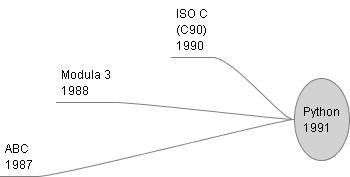
\includegraphics[scale=0.8]{graphics/history.jpg}
	\caption{Einfl�sse anderer Sprachen auf Python}
	\label{fig:history_python}
\end{figure}

Abbildung \ref{fig:history_python} zeigt eine kompakte �bersicht zur Entwicklung Pythons. Eine detaillierte, historische �bersicht zur Entstehung von Programmiersprachen im Allgemeinen ist auf \cite{python:pix} zu finden.

Python wird 1991 ver�ffentlicht; die Entwicklung der ersten Version geht bis Python 1.6.1. Oktober 2000 wird Python 2.0 freigegeben, zum Zeitpunkt dieser Arbeit ist Python in Version 2.5 aktuell, welche seit September 2006 zur Verf�gung steht. Momentan wird an Version 3.0 (Py3K, Python 3000) entwickelt, die in einer \emph{Alpha} Version 2007 erwartet wird\footnote{Python 3000, Google Tech Talk, Guido van Rossum, 2006}.

Diese Arbeit greift nun den Versuch auf, die Popularit�t Pythons anhand einer Google Suche zu messen. Das ist keine sehr wissenschaftliche Messung, spiegelt aber doch eine gewisse Relevanz und vor allem deren Ver�nderung in den letzten Jahren, in der weltweit gr��ten Suchmaschine wider. Basis der Untersuchung sind die Ergebnisse aus dem Jahr 2002 von \cite{python:teachingscientific}:

\begin{table}[h]
	\centering
	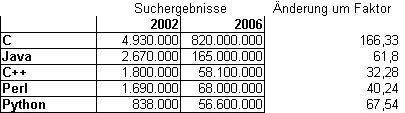
\includegraphics[scale=0.75]{graphics/google1.jpg}
	\caption[Google Vergleich 1]{Google-Suche: {\tt Platzhalter-Sprache AND ( language OR code OR program)}. Zugriff auf http://www.google.com/ am 22.10.2006.}
	\label{fig:google1}
\end{table}

Tabelle \ref{fig:google1} stellt die Ergebnisse einer Anfrage an die Suchmaschine Google dar. Dabei wird die urspr�ngliche Anfrage von \cite{python:teachingscientific} aus dem Jahr 2002 mit der gleichen - nur zeitlich aktuelleren - Anfrage verglichen. Wie zu erkennen ist, ist die Anzahl der Treffer immens in die H�he geschnellt. Das kann in erster Linie durch die technologische und inhaltliche Entwicklung der Suchmaschine begr�ndet werden, wie auch durch die Relevanz der einzelnen Suchanfragen.
\\Die hohe Trefferanzahl der Sprache C ist mit Vorsicht zu genie�en, da angenommen werden kann, dass hier einige Treffer zu C++ mitgerechnet werden. Trotzdem steht C ungeschlagen an der Spitze dieser Auswertung, was auch nicht weiter verwunderlich ist. Nach wie vor wird C in der Systemprogrammierung verwendet, Schnittstellen zu Anwendungsprogrammen sind typischerweise ebenso in C implementiert. Ein C-Compiler exisitiert f�r eine Vielzahl an Plattformen. Gerade im rasant gewachsenen Embedded Systems Bereich ist C quasi Standard.
\\Die anderen Programmiersprachen sind interessant zu beobachten, wobei Python im Vergleich zu 2002 das gr��te Wachstum verbuchen kann und sich im Gesamtvergleich mit Anwendungsentwicklungssprachen wie C++ oder Java durchaus messen kann. Im Vergleich der Skriptsprachen hat Perl vor Python die h�here Trefferanzahl.

\begin{table}[h]
	\centering
	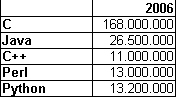
\includegraphics[scale=0.75]{graphics/google2.jpg}
	\caption[Google Vergleich 2]{Google-Suche: {\tt Platzhalter-Sprache AND ( (language OR code OR programm) AND ( education OR teaching))}. Zugriff auf http://www.google.com/ am 22.10.2006.}
	\label{fig:google2}
\end{table}

Die Daten in Tabelle \ref{fig:google1} sind sehr allgemein und umfassen mehr als die gew�nschte Thematik dieser Arbeit. Aus diesem Grund wird mit Tabelle \ref{fig:google2} die Suchanfrage leicht abge�ndert und damit konkretisiert: wie relevant sind die genannten Programmiersprachen im Unterricht? W�hrend Tabelle \ref{fig:google1} die Ver�nderung im Laufe der letzen Jahre darstellt, zeigt Tabelle \ref{fig:google2} den Status quo.
%TODO ? {\color{red} eventuell verweis auf \ref{kapitel:Programmiersprachen}}

Weiterf�hrende Literatur zu Python: \cite{python:website}, \cite{python:bytesofpython}, \cite{python:thinkCS}, 			\cite{python:programming_python}, \cite{python:cookbook}, \cite{python:diveinto}.

		\subsubsection{High-Level-Sprache und Skriptsprache}
			\HLL\ nach \cite{misc:hll, python:linkweiler}: 
\begin{quote}
{\itshape "'A computer programming language that is primarily designed for, and syntactically oriented to, particular classes of problems and that is essentially independent of the structure of a specific computer or class of computers."'}
\end{quote}

Nach diesem Zitat ist eine \HLL\ eine Programmiersprache, die unabh�ngig von der Maschine ist. Programmiersprachen ab der dritten Generation z�hlen zu den h�heren Programmiersprachen oder High-Level-Languages. In der Literatur wird oft auch der Begriff "'Systemsprache"' verwendet. Eine \HLL\ hat eine f�r Menschen lesbare Syntax, die von einem Compiler oder Interpreter 1:n in Maschinensprache �bersetzt wird. Das bedeutet, dass ein einziger Befehl in einer \HLL\ durch viele Instruktionen in Maschinensprache ausgedr�ckt wird. Assembler, z�hlend zur zweiten Generation, �bersetzt 1:1 in Maschinensprache, die wiederum zur ersten Generation gez�hlt wird.

Zwei verschiedene Programme verarbeiten eine \HLL\ in Maschinensprache (Bin�rcode): Compiler und Interpreter. Ein Interpreter liest ein High-Level Programm und f�hrt es aus. Die Analyse des Quelltextes erfolgt also zur Laufzeit des Programms.

\begin{figure}[h]
	\centering
	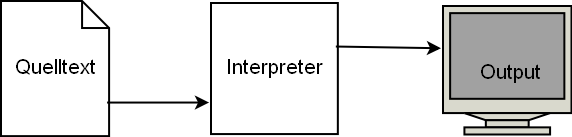
\includegraphics[scale=0.4]{graphics/interpreter.png}
	\caption{Interpreter}
	\label{fig:interpreter}
\end{figure}

Ein Compiler analysiert das Programm und �bersetzt es komplett, bevor das Programm ausgef�hrt wird. Der somit entstandene Code wird Objektcode genannt. Das Programm kann ohne weitere �bersetzung wiederholt ausgef�hrt werden.

\begin{figure}[ht]
	\centering
	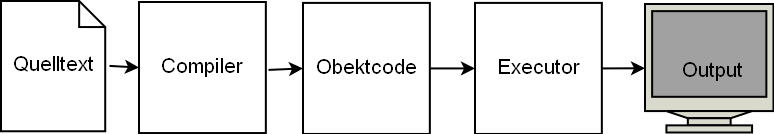
\includegraphics[scale=0.4]{graphics/compiler.png}
	\caption{Compiler}
	\label{fig:compiler}
\end{figure}

Python wird zu den interpretierten Programmiersprachen gez�hlt; Programme werden von einem Interpreter ausgef�hrt. Es gibt hierbei zwei Varianten: den Kommandozeilenmodus und den Skriptmodus. Im Kommandozeilenmodus werden Befehle Zeile f�r Zeile eingegeben, der Interpreter gibt das Ergebnis sofort retour\footnote{Im Laufe der Arbeit werden immer wieder Quelltexte eingearbeitet. Dabei gibt es zwei Formen. Die interaktive Session einer Interpreter Shell und den Skriptmodus. Die Interpreter Sessions sind erkennbar an der typischen Python Eingabeaufforderung (engl. "'prompt"'), die durch drei aufeinanderfolgende spitze Klammern ($>>>$) symbolisiert wird. Die Eingabe ist dabei immer fett ausgepr�gt, die Ausgabe des Interpreters normal.}:

\begin{lstlisting}[style=interpreter, label=python:first_example]
$ python
Python 2.4.4c1 (#1, Oct 13 2006, 12:10:43)
Type "help", "copyright", "credits" or "license" for more information. 
>>> print 10 * 2 
20
\end{lstlisting}

Im Skriptmodus wird das Programm in einem File gespeichert. Der Inhalt wird dann vom Interpreter ausgef�hrt.

Der Skriptmodus f�hrt zum Begriff Skriptsprache. Wie zu Beginn des Kapitels erw�hnt, wird Python den interpretierten Skriptsprachen zugeordnet.
Eine Skriptsprache ist eine \HLL\/, jedoch mit noch h�herer Abstraktion zur Maschine. \cite{python:scriptinglanguages} unterscheidet dabei Systemsprachen von Skriptsprachen wie folgt:
\begin{quote}
{\itshape "'Scripting languages are designed for different tasks than system programming languages, and this leads to fundamental differences in the languages. System programming languages were designed for building data structures and algorithms from scratch, starting from the most primitive computer elements such as words of memory. In contrast, scripting languages are designed for gluing: they assume the existence of a set of powerful components and are intended primarily for connecting components together. [...] Scripting languages are sometimes referred to as glue languages or system integration languages. [...] The growth of the Internet has also popularized scripting languages. The Internet is nothing more than a gluing tool."'}
\end{quote}

Skriptsprachen haben andere Aufgaben als "'Systemsprachen"'. Sie sind nicht darauf ausgelegt Datenstrukturen oder Algorithmen von Grund auf neu zu entwickeln, sondern als Bindeglied f�r vorhandene Applikationen zu dienen. Skriptsprachen bedienen sich also anderer Komponenten, um daraus eine eigene Applikation entstehen zu lassen.

Den immer wieder kritisierten Geschwindigkeitsunterschied zu kompilierten Sprachen versuchen Skriptsprachen wie Python zu verbessern. So wird der Quelltext nicht direkt interpretiert, sondern zuerst in den sogenannten "'Bytecode"' umgewandelt. Dieser wird wesentlich schneller interpretiert. Wirklich Geschwindigkeitskritisches  oder Rechenintensives wird in einer kompilierten Sprache geschrieben. Wie schon erw�hnt, wird bei Python C verwendet. Weiters relativiert immer schnellere und billigere Hardware die Kritik an der Performance.

Einige weitere Eigenschaften von Skriptsprachen sind in diesem Kapitel schon erw�hnt. Zur �bersicht sei eine Darstellung in kompakter Form aufgelistet:
\begin{itemize}
	\item noch "'h�here"' Implementierung als eine typische \HLL\
	\item interpretiert
	\item dynamische Typverwaltung
	\item optimal f�r schnelle Softwareentwicklung bzw. Prototyping \cite{python:linkweiler}
	\item hoher Re-Use Faktor
	\item leichter erlernbar als Systemsprachen
\end{itemize}

Weitere Beispiele f�r Skriptsprachen sind Perl\footnote{Perl: http://www.perl.com/} oder Tcl\footnote{Tcl: http://www.tcl.tk/}.		
		
	
	\subsection{Grundlagen Zope}
		\label{sec:Grundlagen_Zope}
		%\subsubsection{Was ist Zope}
		%Nicht-Fokus: Featureliste.

\Zope\/\footnote{Zope: http://www.zope.org/} ist ein Applikations- und Backend Server Framework, das Entwicklern erlaubt, schnell Protokolle einzubinden, Applikationen (�blicherweise webbasierte) zu entwickeln, und Konnex zwischen anderen internetbasierten Services herzustellen \cite{zope:richter}.

Zope wird gro�teils mit Python entwickelt. Geschwindigkeitskritisches wird in C umgesetzt. �blicherweise wird die mit Zope mitgelieferte \ZODB\ verwendet, um transaktionssicher\footnote{siehe Maillinglisteneintrag "'ZODB implementiert kein ACID"': https://mail.dzug.org/pipermail/zope/2007-June/003937.html} (Python) Objekte zu persistieren. Zope ist mit der \ZPL\/\footnote{Zope Public Licence: http://www.zope.org/Resources/ZPL/}, einer freien Softwarelizenz, verf�gbar.

Momentan werden zwei stabile Zope Versionen von der Community gepflegt. Mit Oktober 2006 ist Zope 2.10 die letzte stabile Version der Zope 2 Generation. Zope 3.3 ist die letzte stabile Version des neuen Zope 3. Diese Arbeit konzentriert sich auf Zope 3, wobei zuerst einige Unterschiede zu Zope 2 aufzeigt werden sollen.

\subsubsection{Zope 2}

Bevor Zope ins Leben gerufen wird, entwickelt die Zope Corporation\footnote{http://www.zope.com/} (urspr�nglich Digital Creations) 1996 das Produkt Bobo, ein in Python entwickelter Object-Publisher, welcher Entwicklern erlaubt, Python Objekte im Web abzubilden. Bobo ist weiters eine Objektdatenbank und ein \ORB\/, der \URL\ in Objektpfade umwandelt. 1998 wird dieses Produkt als Open-Source unter dem Namen Zope ver�ffentlicht.\cite{zope:richter}

Zope 2 erfreut sich anfangs gro�er Beliebtheit durch die \TTW\ Entwicklung und Administration. Komplette Projekte k�nnen per Web entwickelt werden, ohne auch nur einmal eine Kommandozeile zu sehen. Die schnelle Projektabwicklung durch die Produktivit�t mit Python plus die Zope Templatesprachen \DTML\ und \ZPT\ mobilisieren viele Entwickler, ihre Projekte mit Zope umzusetzen.

Zope 2 hat jedoch mit einer Vielzahl von Problemen zu k�mpfen. Die anfangs, vor allem bei unerfahrenen Entwicklern, sehr beliebte \TTW\ Entwicklung st��t schnell an Grenzen. So muss f�r fortgeschrittenere Methoden, wie etwa das Verwenden von regul�ren Ausdr�cken, das Zope 2 Sicherheitssystem umgangen werden. Zope 2 \TTW\ wird vom Framework aus Stabilit�tsgr�nden mit eingeschr�nktem Zugriff auf Pythonbibliotheken versehen. Mit Zope 3 gibt es hier keine Einschr�nkung, da Funktionalit�t mit Hilfe von Pythonpaketen implementiert wird. Innerhalb dieser Pakete kann auf die komplette Funktionalit�t Pythons zur�ckgegriffen werden. Das ist unter Zope 2 auch m�glich, nur ist die Dokumentation dazu schlecht zug�nglich und die Implementierung nur mit einigen Tricks m�glich. Listing \ref{zope:zope2contentclass} zeigt ein Beispiel dazu: wird das Initialisieren der Klasse in Zeile 27 vergessen, ist schnell und einfach eine potentielle Sicherheitsl�cke produziert. Das Zope 2 Framework liefert dem Entwickler hierzu keine Hinweise oder Warnungen.

\begin{lstlisting}[style=example, caption={Typische Zope 2 Content Klasse}, label=zope:zope2contentclass]
from Globals import DTMLFile, InitializeClass
from OFS.SimpleItem import SimpleItem
from OFS.PropertyManager import PropertyManager

class Contact(SimpleItem, PropertyManager):
	
	def __init__(self, first, last, address, postal_code):
		self.manage_edit(first, last, address, postal_code)
	
	manage_options = (SimpleItem.manage_options +
	PropertyManager.manage_options
		+ ({'label': 'Edit', 'action': 'manage_main'},
		   {'label': 'View', 'action': 'index_html' },))

	security.declareProtected('Change Contacts', 'manage_main')
	manage_main = DTMLFile('dtml/main', globals())
	
	security.declareProtected('View', 'index_html')
	index_html = DTMLFile('dtml/index_html', globals())

	security.declareProtected('Change Contacts', 'manage_edit')
	def manage_edit(self, first, last, adress, postal_code, REQUEST=None):
	...
	if REQUEST is not None:
		REQUEST.RESPONSE.redirect(...)
		
	InitializeClass(Contact)
\end{lstlisting}

Um existierende Funktionalit�t zu erweitern, muss unter Zope 2 das sogenannte "`Monkey-Patching"' angewandt werden.  Hierbei wird die urspr�ngliche Funktionalit�t zur Laufzeit ge�ndert, ohne den Originalquelltext zu ver�ndern. Eine gef�hrliche Methodik, da der Monkey-Patch nach einer �nderung des Originalquelltextes, mit hoher Wahrscheinlichkeit nicht mehr funktional ist. Bei exzessiver Anwendung dieser Methodik kommt der Entwickler schnell in Teufels K�che. Konkurrierende Monkey-Patches sind schwer nachvollziehbar, die Wartung wird somit teuer erkauft. 

Auch die schlechte Trennung von Inhalt, Konfiguration und Pr�sentation tr�gt einen Teil dazu bei. Unter Zope 2 muss jede Instanz einer Klasse Attribute und Methoden bereitstellen, die Zope f�r die Interaktion im Framework ben�tigt. Das f�hrt zu �berladenen Objekten, schr�nkt die Portierbarkeit ein und erschwert nachtr�gliche Erweiterungen.\cite{zope:linuxmagazine1}

Trotzdem sind in den letzten Jahren hunderte von sogenannten Produkten unter Zope 2 ver�ffentlich worden. Die Palette reicht von einfachen Erweiterungen, wie z.B. unterschiedliche Datenbankadapter, Wikis, Blogs, bis zu e-Commerce L�sungen. Seine Praxistauglichkeit stellt Zope 2 etwa im Intranet-Einsatz der \NATO\ oder beim Webauftritt des \WWF\/\footnote{WWF: http://www.wwf.at/} unter Beweis. Auch bekannte Contentmanagementsysteme wie Plone\footnote{Plone: http://www.plone.org/} oder der \CPS\/\footnote{CPS: http://www.cps-project.org/} st�tzen sich auf Zope.\cite{zope:ctarticle1}

F�r mehr Literatur zu Zope 2 empfiehlt der Autor \cite{zope:bible}, \cite{zope:book}.

\subsubsection{Zope 3}

Dieses Kapitel umfasst die allgemeinen Eigenschaften und Merkmale von Zope 3. Tiefergehende Informationen und Praxisbezug sind in Kapitel \ref{sec:zope} zu finden.

Das Zope 3 Projekt wird im Februar 2001 ins Leben gerufen. Die Community spricht sich f�r eine komplette Neuentwicklung des Frameworks aus, um die grundlegenden Schwierigkeiten mit Zope 2 auszumerzen. Seit Oktober 2005 ist Zope 3 auch f�r den Produktionseinsatz freigegeben.

Die Komponentenarchitektur, als wichtigeste Neuerung, teilt die Zust�ndigkeit f�r Inhalt (Content), Dienste (Utilities), Sichten (Views) und Adapter auf. Sie erm�glicht es, Software in kleinen und wiederverwertbaren Bausteinen zu entwickeln. Ziel einer solchen Aufteilung ist vor allem die h�here Wartbarkeit der Software. Ein anderes Datenbank-Backend, oder ein neuer Skin f�r eine Webapplikation soll keine Konsequenzen auf die tats�chliche Programmlogik haben. Au�erdem wird f�r eine gewisse �bersicht und Ordnung durch Reduzierung der Komplexit�t gesorgt.

Auch die Wiederverwendung existierender Python-Komponenten aus den Bibliotheken gestaltet sich einfacher, als in der Vorg�ngerversion. Das d�rfte helfen, die bisher vorhandene Spaltung zwischen Python- und Zope-Entwicklern zu �berwinden \cite{zope:ixarticle1}.

Damit Komponenten austauschbar bleiben, m�ssen ihre Schnittstellen definiert sein. Daf�r zust�ndig sind Interfaces, die als Vertr�ge f�r die Komponenten fungieren. So ist es m�glich, dass unterschiedliche Implementierungen f�r ein Interface entwickelt werden k�nnen, da ein Interface nur das "`Was"' beschreibt, nicht aber das "`Wie"'.

Zope 3 Komponenten kurz beschrieben:
\begin{description}
	\item[Content Komponenten] sind Datenobjekte. Die Daten sind anhand eines Schemas definiert. Ihre einzige Aufgabe besteht darin, ihre Daten zu verwalten. Das erm�glicht eine Zope-unabh�ngige Weiterverwendung unter Python.
	\item[Utilities] Utilities sind kontextunabh�ngige Komponenten, die f�r bestimmte Aufgaben im Framework zust�ndig sind (z.B. Emailversand, Kodierung, Suche).
	\item[Adapter] Adapter nutzen eine Komponente mit definiertem Interface, um ein neues Interface bereitzustellen. Das erm�glicht existierende Funktionalit�ten zu erweitern, ohne die Originalimplementierung zu ver�ndern.
	\item[Views] sind Komponenten, die f�r die Darstellung anderer Komponenten zust�ndig sind. Views sind normalerweise als Kombination von Python-Code f�r Logik und \ZPT\ f�r die Pr�sentation definiert.
\end{description}

Die Konfiguration des Frameworks und der Applikationen erfolgt bei Zope 2 im Quelltext selbst. Ver�nderungen der Konfiguration hat eine �nderung des Quelltextes zur Folge. Zope 3 Konfiguration wird in seperaten \XML\/-Dateien abgelegt. Der verwendete Dialekt ist \ZCML\/.

Um Entwicklern und vor allem bestehenden Applikationen die Umstellung auf Version 3 zu erm�glichen, wurde das Projekt Five (Zope 2 + Zope 3 = Five) ins Leben gerufen. Five ist ein Zope 2 Produkt, das einiges an Zope 3 Funktionalit�t zur Verf�gung stellt. Zuk�nftige Zope 2 Versionen und Five werden langsam zu einer gemeinsamen Zope Version, basierend auf Zope 3, f�hren.

Der Gro�teil der momentanen Zope Projekte basiert auf Version 2. Anhand des stark wachsenden Interesses in den Communityforen und Mailinglisten\footnote{Zope Users Mailingliste: http://mail.zope.org/pipermail/zope3-users/}, und der stetig steigenden Anzahl an Zope 3 Modulen im Zope Repository\footnote{Zope Repository: http://svn.zope.org/}, kann in Zukunft mit einer gr��eren Anzahl an Referenzen gerechnet werden. Ende 2006 sind folgende gr��ere Projekte bekannt:
\begin{description}
	\item[Schooltool]\footnote{Schooltool: http://www.schooltool.org/} ist eine Applikation f�r die Administration einer Schule.
	\item[Launchpad]\footnote{Launchpad: https://launchpad.net/} ist ein Framework rund um Opensource Produkte, wie die Linux Distribution Ubuntu\footnote{Ubuntu: http://www.ubuntu.com/} oder die Versionierungssoftware Bazaar\footnote{Bazaar: http://bazaar-vcs.org/}.
\end{description}
 
Weiterf�hrende Zope 3 Literatur: \cite{zope:weitershausen}, \cite{zope:richter}

				
		
\newpage
\section{Python lehren}
\rkopf[]{Python lehren}
	\subsection{Python als erste Programmiersprache?}
		\label{sec:firstlanguage}
		Warum eignet sich Python als Werkzeug f�r den Informatikunterricht? Ist Python als Einstiegssprache geeignet? Was zeichnet Python gegen�ber anderen Programmiersprachen aus? Welche Anforderungen werden an eine "'erste Programmiersprache"' gestellt? Was haben die Lehrenden davon? Dieses Kapitel enth�lt eine Diskussion zu den vorangegangen Fragen. 

Gegenw�rtig sind haupts�chlich Java und C++ als Programmierprachen in Lehrg�ngen f�r Programmieranf�nger anzutreffen (vgl. Kapitel \ref{kapitel:Programmiersprachen}) \cite{python:firstlanguage6}.

\begin{quote}
{\itshape "'While students with good preliminary background, who have already committed themselves to a computing career, usually succeed in such courses, many others remain disappointed or even completely fail."'}
\end{quote}

\cite{python:firstlanguage6} schreibt, dass Studenten mit Vorkenntnissen und explizitem Interesse an der Materie es leichter haben, solche Kurse erfolgreich zu absolvieren. Studenten, die bisher keine Erfahrungen in der Programmierung haben, bleiben hier oft auf der Strecke. Die Motivation, die Materie weiter zu verfolgen, ist verst�ndlicherweise gering. Dabei soll Unterricht �blicherweise motivieren und dadurch den Forschergeist wecken. Ob das gelingt, ist eine Frage der Gestaltung des Unterrichts und h�ngt nur geringf�gig von der zu unterichtenden Materie ab. Jedes noch so trockene Thema kann durch interessante und fesselnde Unterrichtsgestaltung schmackhaft gemacht werden. Die Unterrichtsgestaltung h�ngt auch mit der Wahl der benutzten Werkzeuge, um Wissen zu vermitteln, zusammen.

Das Problem nach \cite{python:firstlanguage6} ist, dass die heute verwendeten Sprachen alle kommerziell ausgerichtet sind. Kommerzielle Sprachen sind nicht f�r den Unterricht ausgelegt, sondern f�r die industrielle Softwareentwicklung. Kommerzielle Applikationen sind komplex. Die Programmiersprachen sind daf�r ausgelegt, die Entwicklung dieser Applikationen zu erm�glichen.

Der Autor unterst�tzt diese Argumentation. Es stellt sich jedoch die Frage, warum nicht gerade aus diesen Gr�nden Programmiersprachen so einfach und �bersichtlich wie m�glich sein sollten. Eine Ursache daf�r ist sicher eine versuchte Effizienzsteigerung durch diverse Sprachkonstrukte, die den Profi effizienter arbeiten lassen, f�r Anf�nger aber nicht leicht verst�ndlich sind ("make the common case efficient"). \cite{python:firstlanguage6} meint in seiner Arbeit, dass genau aus diesem Grund Programmierneulinge mit Konzepten konfrontiert werden, die f�r den Anfang �berfordern.

\cite{python:firstlanguage1} bringen einen Vergleich f�r den sportlichen Leser, indem sie ein Beispiel aus dem Schifahren bringen. Um ein wirklich guter Schifahrer zu werden, erfordert es �bung. Schipisten sind darauf ausgelegt, das �ben zu unterst�tzen, indem sie je nach Schwierigkeitsgrad farblich markiert sind. Blau f�r Anf�nger, Rot f�r Fortgeschrittene und Schwarz f�r Profis. Eine blaue Piste bedeutet aber nicht, das hier auf die wichtigen Elemente des Schifahrens zu verzichten ist. Schw�nge, Geschwindigkeitskontrolle, Bremsen und die richtige �bersicht sind auch hier notwendig, sind jedoch unter entsch�rften Bedingungen aus�bbar. Wird ein Anf�nger auf die schwarze Piste geschickt, wird er oft st�rzen. Die Erfahrung ist f�r ihn frustrierend, und er wird schnell aufgeben und den Sport verdammen.

Dieser Ausflug in eine anderes Gebiet und die einfache Erkenntnis daraus kann auf jedes Lernen umgelegt werden. Konfrontiert man den Lernenden zu fr�h mit zu hoher Komplexit�t, kann dieser nicht genug Erfolge erleben und wird sich eher frustriert von der Thematik abwenden. Der Stoff muss sich aufbauend an den fundamentalen Ideen des Unterrichtsgegenstandes n�hern, und dem Lernenden zwischendurch immer wieder Erfolgserlebnisse erm�glichen.

\begin{quote}
{\itshape "'As students progress through the introductory computer science sequence, we want them to
focus on aspects of problem solving, algorithm development, and algorithm understanding.
Unfortunately, many modern programming languages require that students jump into more
advanced programming concepts at a point that is too soon in their development. This
sets them up for possible failure, not because of the computer science but because of the
language vehicle being used."'}\cite{python:firstlanguage1}
\end{quote}

In der Informatik liegt das Augenmerk auf den Aspekten der Probleml�sung, der Entwicklung und dem Verstehen von Algorithmen. Die heute im Unterricht angewandten Programmiersprachen f�hren aber zu fr�h in komplexere Details der Wissenschaft. Das f�hrt auch dazu, dass nicht Informatik, sondern die Aspekte einer Programmiersprache zum Gegenstand des Unterichts werden.

\begin{quote}
{\itshape "'It is a shame that the languages that our students encounter when they come to learn to program are
languages that are designed for commercial use by experienced commercial programmers. Modern languages
like Java and C++ contain a host of features that most students will never need, and which we should
probably admit are a mystery to many of the students' teachers."'}\cite{python:firstlanguage2}
\end{quote}

Sprachen wie Java oder C++ sind in ihrem Umfang so m�chtig, das es bestimmt eher selten ist, wirklich routinierte Profis als Lektoren zu bekommen. Gl�cklich sind diejenigen, die in diesen Genuss kommen. 

\subsubsection*{Industriesprachen}

We�halb werden Java, C++ und C nun haupts�chlich verwendet? Geht es nach \cite{python:firstlanguage2}, \cite{python:CRPITV52P71-80}, \cite{python:firstlanguage7}, \cite{python:industry1}, \cite{python:industry2} und \cite{python:firstlanguage9}, ist dieser Zustand industriegetrieben. Studenten sehen Jobangebote, in denen eine bestimmte Programmiersprache als Voraussetzung verlangt wird, und wollen diese lernen, um ihre Qualifikation damit aufzuwerten. Sie haben kein Interesse, eine "'Baby-Sprache"'\cite{python:firstlanguage11} zu lernen. Lehreinrichtungen bewerten ihre Studienpl�ne anhand der Nachfrage in der Industrie. Das betrifft ganz besonders Fachhochschulen, wo Lehrpl�ne in enger Zusammenarbeit mit der Industrie erstellt werden. 

Ein Lektor des Autors, der lieber anonym bleiben m�chte, ist da ganz anderer Meinung. Die obig gebrachten �berlegungen seien unwahr, vielmehr gestaltet sich der Unterricht oft nach der Verf�gbarkeit von Lektoren im Bekanntenkreis der f�r den Studienplan verantwortlichen Personen. Diese Lektoren bringen eher ihre pers�nlich bevorzugten Themen und Werkzeuge in den Unterricht ein (wobei letzteres durchaus legitim und wichtig f�r die Qualit�t des gebrachten Unterichtsstoffes ist).

Nach Ansicht des Autors ist die Realit�t wohl eine Mischung aus beiden gerade genannten Punkten. Doch sollte es nicht anders sein? In der Informatik war es fr�her auch anders. Blickt man auf die Zeit vor der objektorientierten Bewegung zur�ck, gab es Pascal \cite{misc:pascal} als allgemein anerkannte Programmiersprache f�r den Unterricht \cite{python:firstlanguage6},\cite{python:firstlanguage7}. Das Problem mit reinen Unterrichtssprachen wie Pascal  ist jedoch, dass sie in der Industrie nicht verwendet werden. Aus diesem Grund wurde Pascal auch weltweit aus den Lehrpl�nen gestrichen. 

Es braucht also eine Sprache, die
\begin{itemize}
	\item in der Industrie anerkannt ist bzw. in der Industrie Verwendung findet,
	\item mit der komplexe Softwareprojekte umgesetzt werden k�nnen,
	\item die f�r den Unterrichtseinsatz geeignet ist.
\end{itemize}

Betrachten wir Python, sind die ersten beiden Punkte erf�llt. Wenden wir uns nun dem dritten Punkt zu. Ist Python f�r den Unterrichtseinsatz geeignet?

\subsubsection*{Hello World}

\emph{Hello World} ist traditionellerweise das erste Programm jedes Programmieranf�ngers. Starten wir gleich mit der Python Variante.

\begin{lstlisting}[style=example, caption={Hello World mit Python}, label=python:helloworldpython]
print "Hello World!"
\end{lstlisting}

Nun zur C++ Variante des Programms.

\begin{lstlisting}[style=example, caption={Hello World mit C++}, label=python:helloworldC++]
#include <iostream>

using namespace std;

int main ()
{
  cout << "Hello World!";
  return 0;
}
\end{lstlisting}

\begin{itemize}
	\item Zeile 1: Zeilen, die mit einer Raute(\#) beginnen, sind Direktiven f�r den Pr�prozessor. Diese Zeilen werden vom Compiler nicht normal ausgewertet, sondern zuvor vom Pr�prozessor bearbeitet. Dieser reagiert je nach Befehl unterschiedlich. In diesem Beispiel wird dem Pr�prozessor mitgeteilt, die Datei \verb|iostream| zu inkludieren. Diese enth�lt Deklarationen der Standard Eingabe-Ausgabe Bibliothek von C++. Sie wird ben�tigt, da wir einen Befehl aus dieser Bibliothek sp�ter im Programm verwenden.
	\item Zeile 3: Alle Elemente der Standard C++ Bibliothek werden in einem eigenen Namensraum deklariert. Dieser Namensraum hat den Namen \verb|std|.
	\item Zeile 5: Die \verb|main| Funktion ist der Startpunkt eines jeden C++ Programmes. Eine Funktion wird immer mit runden Klammern definiert. Innerhalb der runden Klammern k�nnen Parameter an die Funktion �bergeben werden. Die geschwungenen Klammern markieren den Bereich der Funktion. Alles innerhalb dieser Klammer wird beim Aufruf der Funktion ausgef�hrt. Vor dem Namen der Funktion steht die Definition des R�ckgabewertes.
	\item Zeile 7: Das ist ein C++ Befehl (statement), den wir �ber eine Library inkludiert haben und einem Namesraum zugewiesen haben. Dieser spezielle Befehl repr�sentiert den \emph{Standard Output Stream} in C++. Das Beispiel zeigt, wie eine Sequenz von Zeichen ("'Hello World!"') in den Stream geschrieben wird. Jeder Befehl muss mit einem Semikolon (;) beendet werden.
	\item Zeile 8: Der \verb|return| Befehl beendet die Funktion, der Returnwert muss vom gleichen Typ wie die Deklaration der Funktion sein. Der Returncode von 0 bedeutet, das die Funktion fehlerfrei ausgef�hrt wurde.
\end{itemize}

Wie zu sehen ist, m�ssen, bei diesem sehr simplen Beispiel, Themen, die f�r einen Anf�nger doch sehr fortgeschritten sind, erl�utert werden. Eine andere, und nach Erfahrung des Autors sehr beliebte Variante um diese Problematik zu umschiffen, ist das gezielte Ignorieren dieser Punkte. Der Vortragende ersucht die Studenten, gewisse Teile des Programmes einfach auszublenden und z.B. nur innerhalb der \verb|main| Funktion zu arbeiten und zu denken.

\begin{quote}
{\itshape "'The C++ version has always forced me to choose between two unsatisfying options: either to explain the \#include,   void main(), \{, and \} statements, and risk confusing or intimidating some of the students right at the start, or to tell them 'just don't worry about all of that stuff now, we will talk about it later' and risk the same thing."'}\cite{python:firstlanguage10}
\end{quote}

Keine der beiden Varianten ist befriedigend. \cite{python:firstlanguage10} beschreibt den Aufwand, ein \emph{Hello World} Programm in ein Skriptum zu verfassen, wie folgt.

\begin{quote}
{\itshape "'There are thirteen paragraphs of explanation of "'Hello, world"' in the C++ version, in the Python version there are only three. More importantly, the missing ten paragraphs do not deal with the "'big ideas"' in computer programming, but with the minutia of C++ syntax. I found this same thing happening throughout the chapters that I have completed so far. Whole paragraphs simply disappear from the Python version of the text because Python's much simpler syntax renders them unnecessary."'}
\end{quote}

\cite{python:firstlanguage10} zeigt damit, dass viel Einf�hrungsarbeit mit C++ auf Spracheigenheiten bezogen ist. Das ist Zeitverschwendung. Studenten k�nnten mit Python viel fr�her zu ersten Erfolgserlebnissen kommen, ohne �ber mysteri�se Gegebenheiten, wie unerkl�rte und nicht verstandene Konstrukte, in den eigenen Programmen zu stolpern.

Bei der Java Version des Programmes wird der Student sofort mit einem fortgeschrittenen Konzept konfrontiert, welches aber das Wissen �ber darunterliegende, objektorientierte Thematik  voraussetzt. 

Der Autor will C++ und Java nicht negativ darstellen. Es soll lediglich aufgezeigt werden, dass ein Start in die Programmierung mit einer der momentan in der Ausbildung verwendeten Sprachen nicht als optimal angesehen werden kann. Ein gro�er Vorteil von Python im Vergleich der \emph{Hello World} Programme, ist die unterschiedliche Anzahl der Konzepte, die verstanden werden m�ssen, um ein erstes Programm zu schreiben. Ein erstes funktionales Programm ist auch ein erstes Erfolgserlebnis und motiviert zu mehr.

\subsubsection*{Syntax}

\begin{quote}
{\itshape "'Compared to languages such as Java or C++, Python has a more intuitive syntax. Python enforces an intended and structured way of writing programs, and the code resembles pseudo code."'}\cite{python:CRPITV52P71-80}
\end{quote}

Entwickler werden unter Python gezwungen, mit Einr�ckung ihres Quelltextes zu arbeiten. Eine Einr�ckung markiert einen Block im Programm. Der Block endet erst mit der Einr�ckung. Bei falscher Einr�ckung wird ein Fehler generiert. Dabei sieht ein Programm in Python fast genauso aus wie das Programm geschrieben in Pseudocode. Das hat den Vorteil, dass Algorithmen einfach nach Pseudocodevorlage implementiert werden k�nnen.

\begin{quote}
{\itshape "'[...] with Python, the Pseudocode is in fact also real code, and already executable."'}
\end{quote}

\cite{python:firstlanguage9} meint sogar, dass mit Python sei Pseudocode auch echter Quelltext, der schon ausf�hrbar ist.

Die Einr�ckung zwingt dazu, strukturiert zu schreiben und f�rdert dadurch ein einheitliches Programmbild, w�hrend in anderen Sprachen verschiedene Schreibstile m�glich sind, die dazu f�hren, dass Richtlinien zur Lesbarkeit entwickelt werden m�ssen.

Programme werden lesbarer, was einige Vorteile mit sich bringt. Lektoren haben es leichter, die Arbeit der Studenten zu evaluieren und finden auch schneller Fehler in Programmen. Da Python keine unterschiedlichen syntaktischen Stile erlaubt, ist es somit f�r Studenten einfacher, an gr��eren Projekten gemeinsam zu arbeiten.\cite{python:firstlanguage10}

\begin{quote}
{\itshape "'Novice programmers find indentation to be quite natural and we have found that it enforces a more readable coding
style than students typically adopt when they can use braces."'}\cite{python:firstlanguage1}
\end{quote}

Listing \ref{c:indent} zeigt ein C++ Beispiel. Frei nach dem Auge w�rde der zweite Befehl zum if-Block geh�ren. Durch das Fehlen der geschwungen Klammern umfasst der Block jedoch nur den ersten Befehl, der zweite wird unabh�ngig von der Verzweigung ausgef�hrt. Dieser Fehler passiert recht h�ufig. Mit Python w�re dieses Beispiel klar, alles Einger�ckte nach der Verzweigung ist dem Block zugeh�rig. Es herrscht eine Art "'nat�rliche Lesbarkeit"'.

\begin{lstlisting}[style=example, caption={Beispiel zur Lesbarkeit von einger�cktem Quelltext}, label=c:indent]
if(t == 1)
	cout << "t is 1";
	t = 2;
\end{lstlisting}

\begin{quote}
{\itshape "'We feel that writing structured programs, which are easy to check, follow and maintain, is one of the main lessons in any programming course. Using Python, this lesson is taught automatically."'}\cite{python:CRPITV52P71-80}
\end{quote}

Lesbaren Quelltext zu schreiben ist ein wichtiges didaktisches Ziel. Durch Python erreicht der Student das implizit.


\subsubsection*{Semantik}

Durch die dynamische Typisierung erspart man sich das Konzept der Deklaration. Der Typ einer Variable wird zur Laufzeit bestimmt. Eine Variable zeigt immer auf ein Objekt. Dieses Konzept ist leichter zu erl�utern und zu verstehen, als die maschinennahe statische Typisierung, wo eine Variable ein Platz im Speicher ist, der zuvor deklariert werden muss. Typisierung ist ebenfalls eine h�ufige Fehlerquelle, auf die anfangs getrost verzichtet werden kann. Auch Zeiger und Speicherverwaltung sind solche Konzepte.

Die Literatur ist sich einig, dass die genannten Konzepte f�r eine erste Programmiersprache nicht notwendig sind, aber trotzdem zu einem sp�teren Zeitpunkt gelehrt werden sollten. Erfahrungen zeigen, dass die Konzepte auch viel einfacher angenommen werden, nachdem Studenten ihre ersten Erfolge mit Python erlebt haben und in der Lage sind, eigene komplexe Programme zu schreiben. Der Umstieg auf eine Hochsprache ist unproblematisch.\cite{python:firstlanguage2, python:firstlanguage5, python:firstlanguage6, python:firstlanguage7, python:firstlanguage10, python:firstlanguage11}

\begin{quote}
{\itshape "'We believe that it is advantageous for beginning students to spend time on the green runs[blaue Piste] learning the rudimentary ideas relating to algorithms and data structures. If you are among those of our colleagues who are frustrated with Java or C++, we encourage you to consider Python and join us on the green runs, it works."'}
\end{quote}

\cite{python:firstlanguage10} nimmt wieder das Beispiel des Schifahrens als Illustration und vergleicht Python als erste Programmiersprache mit dem Fahren auf einer blauen Piste, wo Studenten, unter entsch�rften Bedingungen, das Arbeiten mit Algorithmen und Datenstrukturen lernen.				
 
	\subsection{Programmierparadigmen}
		%TODO {\color{red} Paper download: http://ieeexplore.ieee.org/xpl/freeabs\_all.jsp?arnumber=839221, und http://portal.acm.org/citation.cfm?id=201998.202006}

Das Wort \textbf{Paradigma} kommt aus dem Griechischen und bedeutet Vorbild, Beispiel, Muster oder Abgrenzung. Es hat viele unterschiedliche Bedeutungen, die sich in der Wissenschaft, der Linguistik, Organisationstheorie etc. wiederfinden. F�r diese Arbeit und dieses Kapitel ist das Programmierparadigma interessant:

Ein \textbf{Programmierparadigma} ist das einer Programmiersprache oder Programmiertechnik zugrundeliegende Prinzip. Es ist eine Sichtweise, die zur L�sung eines Problems mittels einer Programmiersprache eingenommen wird.\cite{misc:multiparadigm}

Python ist prim�r eine objektortientierte Sprache, unterst�tzt also das objektorientierte Softwareparadigma:

\begin{quote}
{\itshape "'Python is a dynamic object-oriented programming language that can be used for many kinds of software development."'}\cite{python:website}
\end{quote}

Jedoch ist der Entwickler bei der Verwendung von Python an kein spezielles Paradigma gebunden. Python kann somit als \textbf{Multiparadigmen-Sprache} bezeichnet werden. 

In diesem Kapitel wird auf folgende Paradigmen kurz eingegangen und deren Realisierung mit Python erl�utert:

\begin{itemize}
	\item Imperative Programmierung
		\begin{itemize}
			\item Prozedurale Programmierung
			\item Modulare Programmierung
			\item Objektorientiere Programmierung
		\end{itemize}
	\item Deklarative Programmierung
		\begin{itemize}
			\item Funktionale Programmierung
  		\item Logische Programmierung
  	\end{itemize}
  \item Weitere Paradigmen
    \begin{itemize}
		  \item Design by Contract
		  \item Aspektorientierte Programmierung
		  %\item Komponentenortientierte Programmierung
    \end{itemize}
\end{itemize}

\subsubsection{Programmierparadigmen im Unterricht}

Nach \cite{misc:placer} und \cite{misc:westbrook} sind Multiparadigmensprachen f�r den Unterricht gut geeignet. Es ist wichtig den Studenten in kein Korsett hineinzuzwingen, sondern ein breites Schema an M�glichkeiten zur kreativen Entfaltung anzubieten, denn

\begin{quote}
{\itshape "'verschiedene Menschen nehmen zur L�sung von gleichen Aufgaben unterschiedliche Sichtweisen ein, und ebenso kann es sein, dass ein Mensch f�r unterschiedliche Aufgaben verschiedene L�sungsans�tze verfolgt. F�r die wenigsten Probleme gibt es die optimale L�sung, und so empfiehlt es sich, der- oder demjenigen, der das Problem l�st, die Wahl zu �berlassen, wie er oder sie am besten mit einer Aufgabe umgeht. Daher ist es f�r den praktischen
Einsatz von Programmiersprachen notwendig, diese unterschiedlichen Sichtweisen, die zu verschiedenen L�sungsstrategien f�hren, in geeigneter Form ausdr�cken zu k�nnen."'}\cite{misc:multiparadigm}
\end{quote}

Das bietet den Studenten den Freiraum, zu Beginn ihrer Programmierkarriere mittels \textbf{eines} Werkzeugs, n�mlich der Programmiersprache,  unterschiedliche Denkweisen und Programmierans�tze zu erproben. Die Studenten k�nnen sich voll und ganz auf das Verstehen der, den Paradigmen zugrundeliegenden Prinzipien konzentrieren und begreifen, dass ein Paradigma nicht von der verwendeten Programmiersprache abh�ngt, sondern von der Sichtweise auf eine Problemstellung und deren L�sung.

\begin{quote}
{\itshape "'Python erm�glicht sowohl den Logo-Zugang mit Rekursion und Listen, als auch den sequentiellen Zugang der imperativen Sprachen (und wer will - es geht auch funktional). Sprachen wie Delphi oder C++ zwingen den Sch�ler erst einmal, 'nur nichts falsch' zu machen. Das mag Sprach-Juristen erfreuen, l�sst aber den Forschungsdrang der Sch�ler verk�mmern."'}\cite{misc:urban}
\end{quote}

\subsubsection{Imperative Programmierung}

Imperative Programmierung ist das �lteste Programmierparadigma und ist an die Architektur 
des Von-Neumann-Rechners angelehnt. Ein Programm ist eine Folge von Anweisungen, die nacheinander abgearbeitet werden; dieses befindet sich zu jeder Zeit in einem Zustand, der vom Arbeitsspeicher und der Programmumgebung (Dateisystem, 
Peripherie) definiert ist. Seiteneffekte (Ein-/Ausgabe, Speichermodifikation, Variablen) bewirken 
eine �nderung des Zustandes �ber der Zeit.

\paragraph*{Prozedurale Programmierung}

Die prozedurale Programmierung, die als Synonym f�r imperative Programmierung gesehen werden kann,  
erm�glicht das Zusammenfassen von Anweisungen zu Unterprogrammen (Prozeduren). Unterprogramme
werden dann von verschiedenen Stellen des Programms aufgerufen und ausgef�hrt.

Das ist der erste Ansatz, Aufgaben in Teilaufgaben zu zerlegen und so eine einfachere, �bersichtlichere und vor allem wiederverwertbare Programmierung zu erm�glichen.

Es bietet sich an, dieses Paradigma als erstes im Unterricht vorzustellen, da Von-Neumann �blicherweise
sehr fr�h im Informatikunterricht ein Thema ist, und so ein einfacher Konnex hergestellt werden kann.

Um den zeitlichen Ablauf eines Programmes zu veranschaulichen, kann der Python Interpreter als 
unterst�tzendes Visualisierungswerkzeug im Unterricht verwendet werden:

\begin{lstlisting}[style=interpreter]
>>> fahr = 0
>>> while (fahr < 120):
...		celsius = 5./9 * (fahr - 32)
...		print 'Fahrenheit %6.1f = Celsius %6.3f' % (fahr, celsius)
...		fahr += 20
...
Fahrenheit    0.0 = Celsius -17.778
Fahrenheit   20.0 = Celsius -6.667
Fahrenheit   40.0 = Celsius  4.444
Fahrenheit   60.0 = Celsius 15.556
Fahrenheit   80.0 = Celsius 26.667
Fahrenheit  100.0 = Celsius 37.778
\end{lstlisting}

Die prozedurale Variante des obigen, sehr simplen, Beispiels erg�be dann mit ausgelagerter Berechnung:

\begin{lstlisting}[style=example, caption={Prozedurales Programmierbeispiel}, label=python:prozedural]
def fahr2cels(fahr):
	celsius = 5./9 * (fahr - 32) 
	print 'Fahrenheit %6.1f = Celsius %6.3f' % (fahr, celsius) 
	return celsius
  
fahr = 0
while (fahr < 120):
	fahr2cels(fahr)
	fahr += 20
\end{lstlisting}

\paragraph*{Modulare Programmierung}

Modulare Programmierung geht einen Schritt weiter und zerlegt die Prozeduren zusammen mit Daten in logische Einheiten: die Module. Der n�chste Schritt ist, Aufgaben in gr��eren Softwareprojekten zu abstrahieren. Die jeweiligen Module werden einzeln geplant, entwickelt und getestet.

Mit Python ist jede Datei ein eigenes Modul. Ein Verzeichnis mit Modulen wird Package\footnote{http://docs.python.org/tut/node8.html} genannt. Die Python Standardbibliothek und alle Erweiterungen werden als Packages entwickelt und eingebunden.

Wenn die Prozedur aus Listing \ref{python:prozedural} in eine eigene Datei names \verb|mymodule.py| ausgelagert wird, muss diese als Modul eingebunden werden:

\begin{lstlisting}[style=interpreter]
>>> from mymodule import fahr2cels
>>> fahr2cels(0)
Fahrenheit    0.0 = Celsius -17.778
\end{lstlisting}

Um das Modul nun f�r externe Pythonmodule zug�nglich zu machen, muss die Datei \verb|__init__.py| erstellt werden, die das Verzeichnis als Pythonpackage markiert.
Importiert wird das Modul auf unterschiedliche Arten. Dazu ein Beispiel:

\begin{lstlisting}[style=interpreter]
>>> from mydirectory.mymodule import fahr2cels
\end{lstlisting}

Das Kennenlernen der Modularisierung f�rdert das Verst�ndnis der Austauschbarkeit und Wiederverwendbarkeit von Software in einem sehr fr�hen Stadium des Unterrichts. Ohne viele Vorkenntnisse kann der Sinn und Zweck einer solchen Aufteilung erl�utert werden. Zu diesem Zweck k�nnten sich jeweils zwei Gruppen von Studenten zusammenfinden, die unterschiedliche Aufgaben zu l�sen haben. Die Aufgabe ist, ein Programm mittels eines weiteren Moduls zu entwerfen. Dieses Modul wird trotz unterschiedlicher Aufgabenstellung von beiden Studentengruppen ben�tigt. Interessant ist, die Studenten im ersten Anlauf unwissend in den Einzelgruppen arbeiten zu lassen. Danach werden die "Partnergruppen"' einander vermittelt und die jeweiligen, sicher unterschiedlich implementierten, L�sungen des Moduls von den Studenten zu einem gemeinsamen Modul angeglichen. Nat�rlich wird das nicht ganz friktionsfrei von statten gehen. Die �nderungen werden mit gro�er Wahrscheinlichkeit auch die beiden Programme der Gruppen betreffen.

Im zweiten Anlauf setzt man, mit neuer Aufgabenstellung,  die Studenten schon vorher �ber ihre jeweiligen Partner in Kenntnis. Nun soll ein gemeinsames Modul konzipiert werden, bevor man sich �ber die eigene Implementierung im Detail Gedanken macht. Die Schlu�folgerungen daraus werden anschlie�end diskutiert, die Studenten haben die ersten Untiefen der kollektiven Softwareentwicklung erlebt.

\paragraph*{Objektorientierte Programmierung}

Die \OOP\ erweitert das prozedurale Paradigma um Objekte. 

\begin{quote}
{\itshape "'Ein Objekt ist ein Gegenstand des Interesses, insbesondere einer Beobachtung, Untersuchung oder Messung. Objekte k�nnen Dinge, Personen, oder Begriffe sein [...] ein Objekt besitzt einen bestimmten Zustand und reagiert mit einem definierten Verhalten auf seine Umgebung [...] jedes Objekt besitzt eine Identit�t, die es von anderen Objekten unterscheidet [...] ein Objekt kann ein oder mehrere andere Objekte kennen."'}\cite{Balzert2004}
\end{quote}

Heide Balzert schreibt weiters, dass der Zustand eines Objektes dessen Attribute und die jeweiligen Verbindungen zu anderen Objekten umfasst. Das Verhalten eines Objektes wird durch die Menge seiner Operationen (Methoden, Funktionen) beschrieben. Eine �nderung oder eine Abfrage des Zustandes ist nur mittels Operationen m�glich (Geheimnisprinzip). Objekte werden durch Klassen definiert und k�nnen ihre Eigenschaften und Operationen vererben, was eine Schachtelung des Quelltextes erm�glicht.

Folgendes Listing zeigt eine typische Python Klasse:

\begin{lstlisting}[style=example, caption={einfache Python Klasse}]
class Bankkonto:

   def __init__(self,startbetrag):
      """Konstruktor"""
      self.kontostand = startbetrag

   def einzahlung(self, betrag):
      self.kontostand = self.kontostand + betrag

   def auszahlung(self, betrag):
      self.kontostand = self.kontostand - betrag

   def anzeigen(self):
      print self.kontostand
\end{lstlisting}

Wie zu Beginn dieses Kapitels erw�hnt, ist Python eine objektorientierte Programmiersprache. In Python ist alles ein Objekt, wie folgendes Beispiel zeigt.

\begin{lstlisting}[style=interpreter]
>>> konto = Bankkonto(100)
>>> Bankkonto
<class __main__.Bankkonto at 0x401dfbcc>
>>> konto
<__main__.Bankkonto instance at 0x401e972c>
>>> konto.anzeigen
<bound method Bankkonto.anzeigen of <__main__.Bankkonto instance at 0x401e972c>>
\end{lstlisting}
%TODO dieses listing l�sst kapitel Weitere Paradigmen rot erscheinen?

Python l�sst sich somit hervorragend f�r den aufbauenden Unterricht einsetzen. W�hrend mit Java ab dem ersten Programm der objektorientierte Ansatz verstanden werden muss, kann bei Python der Unterricht mit dem verst�ndlicheren, prozeduralen Paradigma begonnen werden. Danach arbeitet sich der Unterricht �ber den modularen Ansatz zur Objektorientierung.

Als Abweichung zur \OOP\ Definition ist das Geheimnisprinzip in Python zu sehen. Es gibt keine private/public Schl�sselw�rter. Somit kann jedes Attribut einer Pythonklasse, egal aus welchem Kontext, ge�ndert werden. Es existiert jedoch eine Namensvereinbarung, die Methoden mit doppeltem Unterstrich (z.B. \verb|__auszahlung()|) vor ihrem Namen, Zugriffe au�erhalb der Klasse untersagt. Das mag f�r traditionelle \OOP\ Entwickler eigenartig klingen, f�r den Unterricht scheint es aber keine Einschr�nkung zu sein (siehe Kapitel \ref{sec:firstlanguage}).

\subsubsection{Deklarative Programmierung}

Wie der Name ausdr�ckt, ist ein Programm \emph{deklarativ}, wenn es beschreibt, \emph{was} passiert. Die imperative Programmierung ist das genaue Gegenst�ck, sie beschreibt, \emph{wie} etwas umgesetzt wird. 

In der deklarativen Programmierung wird eine problemerl�uternde Spezifikation geschrieben, die von der Implementierung der jeweiligen Sprache analysiert und abgearbeitet wird. \SQL\ ist eine bekannte deklarative Sprache; eine \SQL\ Abfrage beschreibt gew�nschte Daten bzw. den Retourwert, der tats�chliche Algorithmus wird vom \RDBMS\ dahinter ausgef�hrt. Ein weiteres Beispiel ist \HTML\/; hier beschreibt der Templateentwickler das Aussehen der Webseite mittels Markup, jedoch nicht den tats�chlichen Renderingprozess des Browsers.

Imperative Programme definieren also explizit einen Algorithmus, um das gew�nschte Ergebnis zu erzielen. Deklarative Programme hingegen spezifizieren das Ergebnis und �berlassen  die Umsetzung der Implementierung dahinter.

\paragraph*{Funktionale Programmierung}

In der funktionalen Programmierung wird mit Funktionen gearbeitet. Hierbei ist zu beachten, dass nicht die Funktionen (Unterprogramme, Prozeduren) aus der Informatik, sondern Abbildungen aus der Mathematik gemeint sind.

\textbf{Abbildung} nach \cite{misc:mathe}: 
\begin{quote}
	"'Seien $M, N$ Mengen und jedem $x \in M$ sei genau ein $y \in N$ zugeordnet. Durch $M, N$ und diese Zuordnung wird eine Abbildung von $M$ nach $N$ definiert [...] Abbildungen sind Funktionen, wenn $M$ und $N$ Teilmengen der reellen Zahlen sind."'
\end{quote}

In der Literatur wird, ungeachtet dessen, nur von Funktionen gesprochen. Aus Gr�nden der Einfachheit und des eindeutigen Paradigmennamen, wird auch in dieser Arbeit weiterhin von Funktionen gesprochen.

Ein Programm nach dem funktionalen Paradigma besteht allein aus Funktionsdefinition,

\begin{lstlisting}[style=interpreter]
>>> def square(x): return x*x
...
>>> def twice(f,x):return f(f(x))
...
\end{lstlisting}

Funktionsanwendung 

\begin{lstlisting}[style=interpreter]
>>> square(4)
16
\end{lstlisting}

und Funktionskomposition. Bei der Kompostion werden mehrere Funktionen zusammengesetzt.

\begin{lstlisting}[style=interpreter]
>>> twice(square, 4)
256
\end{lstlisting}

Funktionen k�nnen als Argumente und R�ckgabewerte verwendet werden, man spricht von \emph{Funktionen h�herer Ordnung}.

\begin{lstlisting}[style=interpreter]
>>> square
<function square at 0x401dee64>
\end{lstlisting}

% TODO Funktionen werden im Optimalfall ohne Seiteneffekte implementiert, ...... {\color{red}TODO} siehe auch %info1_komplett.pdf S 145

Python liefert einen Standardsatz an Werkzeugen zur funktionalen Programmierung. Die Befehle \verb|map()|, \verb|filter()|, \verb|reduce()| und \verb|lambda|, ebenso wie die Packages \verb|functools|\footnote{functools: http://docs.python.org/lib/module-functools.html} und \verb|functional|\footnote{functional: http://oakwinter.com/code/functional/}.

Die oben genannten Befehle sind jedoch seit l�ngerem \emph{deprecated} und werden mit Python 3000 durch andere, schon vorhandene Konstrukte, wie \textit{list-comprehensions}, abgel�st\footnote{Python 3000 and reduce(): http://www.artima.com/weblogs/viewpost.jsp?thread=98196}. Eine list-comprehension sei hier als Veranschaulichung in mathematischer und implementierter Form aufgezeigt: $S = \{ x | x \in \mathbb{N}, x^2 < 2000  \} $

Die Implementierung dazu lautet:

\begin{lstlisting}[style=interpreter]
>>> from itertools import count
>>> S = [x for x in count() if pow(x,2) < 2000]
\end{lstlisting}

Die funktionale Programmierung ist sicher nicht f�r Programmieranf�nger zu empfehlen. F�r einen fortgeschrittenen Kurs oder als unterst�tzendes Werkzeug f�r Mathematik oder Physikunterricht ist sie durchaus geeignet. Es kann mit derselben Sprache eine komplett neue Sichtweise erlernt werden.

Weiterf�hrender Literaturhinweis: \cite{DBLP:books/el/leeuwen90/Barendregt90}

\paragraph*{Logische Programmierung}

Bei der logischen Programmierung ist die Logik eines Programmes selbst als Programm zu betrachten. Logik kann als problemnahe und effiziente Programmiersprache verwendet werden. Ein Programm besteht aus einer Menge von Fakten, Regeln und Anweisungen. Folgende schematische Darstellung ist der Grundgedanke der logischen Programmierung:

\begin{center}
$algorithm = logic + control$
\end{center}

Wobei \emph{logic} dem rein logischen (deklarativen) Aspekt, also dem Wissen �ber die Zielsetzung des Algorithmus (auch Spezifikation genannt), und \emph{control} dem prozeduralen Aspekt, also der Strategie der Anwendung von Ableitungsregeln, entspricht. 

\cite{misc:vorlesung} schreibt �ber die Vorteile des logischen Paradigmas wie folgt:

\begin{quote}
{\itshape "'Dem Anf�nger wird ein erheblicher Teil des Programmieraufwandes abgenommen. Er beschreibt
sein zu l�sendes Problem mit Fakten und Regeln, ohne sich um die L�sungssuche
selbst zu k�mmern. Das hat den Vorteil, dass er mit einfachen Anfragen an sein Programm, komplizierte L�sungsmechanismen ausl�sen kann, die er schrittweise erkunden und f�r sich nutzen lernt [..] Es werden rekursive Denk- und Arbeitsweisen, die zu den fundamentalen Ideen der Informatik geh�ren, fast spielerisch erlernt."'}
\end{quote}

Betrachten wir folgendes Beispiel:

\emph{Alle verheirateten M�nner hassen ihre Schwiegerm�tter\\
Hannes ist der Mann von Christa\\
Tanja ist die Mutter von Christa\\
--------------------------------\\
Hannes hasst Tanja\\}

%Pr�dikatenlogik:\\
%f�r alle X ( f�r alle Z( mutter(X) und kind (Y,X) und verheiratet (Z,Y) -> hasst(Z,X))\\
%mutter(tanja) und kind(Christa, Tanja) und verheiratet(Hans, Christa)

Die deklarative Interpretation erlaubt, �ber die logische Korrektheit einer Klausel zu diskutieren. 

$hasst(Z,X)$ gilt, wenn $mutter(X)$ und $kind(Y,X)$ und $verheiratet(Z,Y)$ gelten. Oder auch

\begin{equation*}
\forall X ( \forall Z( mutter(X) \wedge kind(Y,X) \wedge verheiratet(Z,Y) \rightarrow hasst(Z,X))
\end{equation*}

Die prozedurale Interpretation liest die Klausel als Definition einer Prozedur durch eine Reihe von Prozeduraufrufen:

Um $hasst(Z,X)$ zu beweisen, beweise $mutter(X)$, dann $kind(Y,X)$ und schliesslich $verheiratet(Z,Y)$.

Somit sind Programmiersprachen nach dem logischen (deklarativen) Paradigma auch prozedural anzusiedeln und k�nnen daher auch als Multiparadigmen-Sprachen bezeichnet werden. Der bekannteste Vertreter der logischen Programmiersprachen ist \PROLOG\/.

Logische Programmierung wird unter Python nicht unterst�tzt, wenngleich einige Versuche\footnote{http://aspn.activestate.com/ASPN/Cookbook/Python/Recipe/360698 und http://bedevere.sourceforge.net/} und Vorschl�ge\footnote{http://codespeak.net/pypy/dist/pypy/doc/constraints-and-logic.html} in diese Richtung existieren. Die entsprechende \SIG\ enth�lt wenig Information, was mangelndes Interesse signalisiert. Auf dem Gebiet der logischen Programmierung scheint \PROLOG\ der Platzhirsch zu sein. Anscheinend gibt es so gut wie keinen Bedarf, hier zus�tzliches Werkzeug zu schaffen.

\subsubsection{Weitere Paradigmen}

Mit Python k�nnen noch weitere Paradigmen angewandt werden. Diese z�hlen, nach Ansicht des Autors, jedoch nicht zu den fundamentalen Paradigmen, sondern sind Softwaredesignelemente bzw. Konzepte in der Softwareentwicklung.

\paragraph*{Design by Contract}

\cite{python:dbc} erkl�rt \DBC\ mit folgenden Worten:
\begin{quote}
{\itshape "'A systematic approach to building correct software systems [..] an effective framework for quality assurance [...] A method for documenting software."'}
\end{quote}	

\DBC\ ist somit ein Werkzeug, um Fehler in der Softwareentwicklung zu vermeiden, und dient gleichzeitig der Quelltextdokumentation.  Dabei werden mit Vorbedingungen, Nachbedingungen und Invarianten \emph{Vertr�ge} definiert, die zur Laufzeit des Programms �berpr�ft werden. 

In der Programmiersprache Eiffel ist \DBC\ Bestandteil der Programmiersprache selbst. Unter Python ist \DBC\ eine Erweiterung des objektorientierten Paradigmas, die mit Metaklassen\footnote{Python Metaklasse: http://www.python.org/2.2/descrintro.html\#metaclasses} umgesetzt wird. Es existieren fertige Packages\footnote{PyDBC: http://www.nongnu.org/pydbc/}, um \DBC\ zu implementieren.

\paragraph*{Aspektorientierte Programmierung}

\AOP\ ist ebenfalls eine Weiterentwicklung von \OOP\/. Bei \AOP\ wird der Quelltext um eine weitere Ebene, die \emph{Aspekte}, abstrahiert. Aspekte sind Funktionalit�ten, die wenig bis nichts mit den jeweiligen Objekten zu tun haben, aber dennoch oft ben�tigt werden, und deswegen als Aspekte ausgelagert werden. Diese Aspekte k�nnen nun jederzeit zur Laufzeit zugeschalten werden und somit die Funktionalit�t der Objekte erweitern oder ver�ndern. Somit soll die Komplexit�t tief verschachtelter Objekte gelockert werden. Die entwickelte Software wird wartbarer und wiederverwendbarer.\cite{misc:aopspring}

Dieses Paradigma ist im Vergleich zu den bisherig vorgestellten Paradigmen ein sehr junges und wird seinen Einzug in die Lehre erst in einigen Jahren erfahren. Das l�sst sich mit der sogenannten \emph{Tr�gheit der Lehre} erkl�ren. 

\begin{quote}
{\itshape "'It takes several years before ideas developed in research settings can be tested, evaluated, and disseminated to practicing professionals so that they can be used."'}\cite{misc:803190}
\end{quote}	

Relevante Technologien aus der Industrie ben�tigen bis zu zehn Jahre, um tats�chlich fl�chendeckend unterrichtet zu werden. Als Beispiel sei die \UML\ erw�hnt, die 1997 als Standard akzeptiert wird, deren Einzug in die Lehre aber selbst heute noch nicht abgeschlossen ist. Der Vorteil dieses Prozesses ist die nat�rliche Auslese von Modeerscheinungen, was wiederum das Zeitkriterium einer fundamentalen Idee best�tigt.

F�r Python existieren einfach zu integrierende \AOP\ Module wie Pythius\footnote{Pythius: http://pythius.sourceforge.net/}. Teilweise sind diese Module sehr simpel und abstrakt gehalten, sind aber f�r die Untermalung der Theorie im Unterricht vollkommen ausreichend.

%\paragraph*{Komponentenortientierte Programmierung}
%{\color{red} TODO: hier passend? �berhaupt hier erw�hnen? oder einfach im zope kapitel behandeln}
%Pr�dikative und wissensbasierte Programmierung ???				
	
	\subsection{Algorithmen}
		Das Erlernen von grundlegenden Algorithmen ist eines der wichtigsten fachdidaktischen Ziele. Es ist nicht nur ein fach�bergreifendes Konzept, sondern auch ein essentielles Werkzeug, um komplexe Problemstellungen l�sen zu k�nnen. Dabei ist es wichtig, den Studierenden einen Algorithmus auch ausprobieren zu lassen. Das einfache Erl�utern mit nat�rlicher Sprache und Pseudocode, ist zwar als Unterst�tzung und erste Beschreibung notwendig, hat aber nicht den entsprechenden Lerneffekt. Es muss eine Programmiersprache als Hilfsmittel angewandt werden. Dazu eignet sich nat�rlich Python, da man sich durch die einfache und Pseudocode-�hnliche Syntax mehr auf die Implementierung und das Verstehen des Algorithmus konzentrieren kann, als auf das Verstehen der Programmiersprache. Diese Aussage wird durch nachfolgendes Zitat aus \cite{python:chou-pyalgs} gest�tzt.

\begin{quote}
{\itshape "'Design and analysis of algorithms are a fundamental topic in computer science and engineering education. Many algorithms courses include programming assignments to help students better understand the algorithms. Unfortunately, the use of traditional programming languages forces students to deal with details of data structures and supporting routines, rather than algorithm design. Python represents an algorithm-oriented language that has been sorely needed in education. The advantages of Python include its textbook-like syntax and interactivity that encourages experimentation."'}
\end{quote}	

\cite{python:chou-pyalgs} spricht sogar von einer \textit{algorithmus-ortientierten} Sprache, wenngleich dieser Ausdruck etwas �bertrieben erscheint. Jeder Algorithmus l�sst sich in jeder beliebigen Programmierprache implementieren und zeigt die jeweiligen verschiedenen L�sungswege eines Algorithmus auf. \cite{python:chou-pyalgs} scheint damit einfach die Eignung Pythons f�r die praktische Anwendung von Algorithmen im Unterricht unterstreichen zu wollen.
		
	\subsection{Python in Fachgegenst�nden}
		%In welchen Fachgegenst�nden kann Python noch verwendet werden? Vorstellen von m�glichen Einsatzgebieten in der Mathematik oder im Embedded Systems Bereich. 
	%Nicht-Fokus: Auflistung aller M�glichkeiten.
	%Fokus: Auswahl von 2-3 m�glichen Fachbereichen und kurzes Vorstellen dieser. F�r Details wird auf Literatur verwiesen.
	%Embedded Systems (siehe C Standard in Python History)
	
Wie aus den vorangegangenen Kapiteln hervorgeht, eignet sich Python hervorragend f�r den Einsatz im Informatikunterricht. Einerseits ist Python eine optimale Sprache, um das Programmieren zu lehren, andererseits k�nnen die grundlegenden Konzepte wie Programmierparadigmen und Algorithmen gut erarbeitet werden. 
	
In welchen Fachgegenst�nden kann Python noch verwendet werden? Und warum ist es gut, einen Unterrichtsgegestand mit Python zu unterst�tzen?
	
%\subsubsection*{Mathematik}
Diese Fragen sollen an einem Beispiel aus der \textbf{Mathematik} erl�utert werden.

\begin{lstlisting}[style=interpreter]
>>> def dreieckszahl(n):  return n*(n+1)/2
...
>>> [dreieckszahl(n) for n in range(1,10)]
[1, 3, 6, 10, 15, 21, 28, 36, 45]
\end{lstlisting}

\begin{figure}[h]
	\centering
	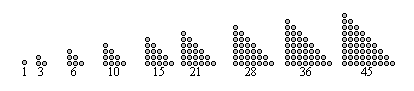
\includegraphics[scale=1]{graphics/dreieckszahl.png}
	\caption{Dreieckszahl}
	\label{fig:dreieckszahl}
\end{figure}

\cite{python:math} bedient sich des Beispiels der Dreieckszahl (Abbildung \ref{fig:dreieckszahl}) und meint, dass der Mathematikunterricht der perfekte Einstieg in das Programmieren ist. 

\begin{quote}
{\itshape "'What I like [...] is the connection between rule-driven (program driven) number sequences, such as 1, 3, 6, 10.. and the corresponding, visually appealing shapes. This forges connections between algebra and visualizations, but in a way more basic than by means of Cartesian coordinates (or any coordinates). Moreover such sequences provide an ideal beginning for learning to program..."'}
\end{quote}

Weiters geht daraus hervor, dass die Verkn�fung von Theorie, praktischer Umsetzung und dem visuellem Feedback durch den Interpreter, oder eine grafische Implementierung\footnote{z.B. mit VPython: http://vpython.org/} den Lernerfolg erh�hen kann.

Diese Aussage wird von \cite{python:broch} gest�tzt, wo es hei�t, dass der h�chste Lernerfolg durch \emph{aktive Lehrmethoden} und \emph{direkt gesteuerte Erfahrung} erzielt wird. Eine aktive Lehrmethode ist z.B. die Erarbeitung und Veranschaulichung der gelehrten Inhalte mittels Python.

%Damit ist die zweite Frage der Einleitung dieses Kapitels beantwortet. Um auch die Erste zu beantworten nennt der Autor noch..

Auch andere Themengebiete der Mathematik lassen sich gut mittels Python unterst�tzen. Induktion, Rekursion, Algebra, Vektoren, Funktionen, Wahrscheinlichkeit und Kryptographie\footnote{Python Cryptography Toolkit: http://www.amk.ca/python/code/crypto} sind nur Ausschnitte m�glicher Teilgebiete.

Folgend nun ein Auszug von Fachgegenst�nden, welche mit Python als unterst�tzendes Werkzeug bereichert werden k�nnen.

\begin{itemize}
	\item \textbf{Betriebssysteme} Prozesse, Threads, Semaphore, Queues, Stacks, ...
	\item \textbf{Internettechnologien} Client-Server Entwicklung, Protokolle, ...
	\item \textbf{Genetik}\footnote{pgapy: http://pgapy.sourceforge.net/ oder Biopython: http://biopython.org/} 
	%\item \textbf{Physik}?? Vpython ist aber schon als Fu�note erw�hnt, einstweilen ausgeblendet
	\item \textbf{3D Engineering}\footnote{Blender: http://www.blender.org/} 
	\item ...
\end{itemize}

Es gibt viele Anwendungsgebiete, und diesen sind auch keine Grenzen gesetzt. Durch die aktive Community und die Offenlegung des Quelltextes ist es m�glich, Python mit fehlender Funktionalit�t zu erweitern. So kann der Unterricht auf die speziellen Bed�rfnisse des Lehrenden angepasst werden.
	
	
%http://hodge.mathematik.uni-mainz.de/~stefan/python/lehrerfortbildung2006.pdf
%http://pgapy.sourceforge.net/ bzw http://www.runtux.com/files/download/pgapy.4.pdf
%http://www.math.uni-siegen.de/ring/mathGUIde/index.html




	
	

	\subsection{Open-Source und Community}
		%http://www.python.org/pycon/dc2004/papers/15/
%http://www.linuxjournal.com/article/5071
%http://portfolio.umaine.edu/~hartt/OS%20in%20Education.pdf

Python ist eine Open-Source Software. Die Community kann als Unterrichtsmaterial angesehen werden sowohl vom Unterrichtenden als auch von den Studenten. Wie kann die Community genutzt werden, was kann sie den Studenten vermitteln?

\begin{quote}
{\itshape "'Die Nutzung von freier Software im Schulunterricht, die u.a. der Begr�nder der Free Software Foundation Richard Stallman fordert, wird seit Jahren durch verschiedene Projekte und Organisationen [...] unterst�tzt. Als Argumente f�r den Einsatz von Open-Source Software dienen dabei vor allem die kostenlose und lizenzrechtlich unproblematische Anschaffung von Betriebssystemen und Programmen sowohl f�r die Schule als auch f�r die einzelnen Sch�lerinnen und Sch�ler, aber auch ethische Aspekte."'}
\end{quote}

\cite{oss:schmeisser} beruft sich auf \cite{oss:freiesoftwareundbildung}, \cite{oss:freesoftware}, \cite{oss:ossgrassmuck}. Dabei ist von freier Software die Rede, die in dieser Arbeit der Open-Source Software gleichgestellt wird. Trotzdem gibt es Unterschiede, die aber nicht Gegenstand dieser Arbeit sind. Weitere Informationen dazu sind bei \cite{oss:neunert} und \cite{oss:osseducation} zu finden.

Python kann somit lizenztechnisch v�llig bedenkenlos an die Studenten verteilt werden; die Installation ist einfach und vor allem kostenlos. Wie schon erw�hnt, gibt es Python f�r diverse Plattformen und Betriebssysteme. Das ist auch ein gro�er Vorteil f�r die Systemadministration des Lehrinstituts, die Python einfach auf allen Rechnern zur Verf�gung stellen kann. 

Als Beispiel m�chte der Autor seine T�tigkeit als Tutor in der \FH\ Technikum Wien erl�utern, wo die Programmiersprache C mit Microsoft Visual C++.net 2005 als Werkzeug gelehrt wird. Die Lektoren dieses Unterrichtsgegenstandes sind hervorragend, jedoch ist die Wahl des Tools mehr als fragw�rdig. Die Probleme w�hrend des Tutorium sind, zu einem nicht unbetr�chtlichen Anteil, Probleme mit dem Werkzeug, das einfach viel zu umfangreich und undurchsichtig f�r die simple Erstellung eines C Programms ist. Die Studenten werden schon allein bei der Installation mit Themen konfrontiert, die zu diesem Zeitpunkt f�r sie unverst�ndlich und deshalb frustrierend sind. Der Compiler meldet C++ Fehlermeldungen, die ohne Hintergrundwissen schwer zu erkl�ren sind. Weiters ist die Installation so aufw�ndig, dass die Software nur in bestimmten R�umen zur Verf�gung steht. Manche Studenten konnten die Installation auf ihren privaten Laptops nicht durchf�hren. Eine Verbesserung w�re das Entwickeln auf einer Linux Shell, wobei nat�rlich ein einf�hrender Unterricht davor notwendig w�re. Alternativ k�nnte z.B. lcc-win32\footnote{lcc-win32: http://www.cs.virginia.edu/\%7Elcc-win32/}, ein Windows C-Compiler mit IDE verwendet werden.

Bei diesem Beispiel schneidet Microsoft Visual C++ nicht gut ab, obwohl das Framework frei zu erwerben ist. Die Software ist jedoch nicht frei, der Quelltext ist nicht zug�nglich. W�re das der Fall, k�nnte theoretisch ein motivierter Student die Unannehmlichkeiten der Installation ausr�umen und hier eine Vereinfachung vornehmen.

Wichtig ist auch, zu erw�hnen, dass freie Software das Erkennen von Konzepten, anstatt das Erlernen von Produkten f�rdert. Es ist m�glich, zu sehen "'wie es andere tun"', und so die eigene Sicht und Arbeitsweise zu verbessern.

Auf die Community kann jederzeit zur�ckgegriffen werden, wenn es um Fragestellungen, Diskussion oder Vorschl�ge geht. Auch kommerzielle Produkte haben Communities, der Autor kann jedoch best�tigen, dass Communities freier Software mit einer komplett anderen Motivation und Hilfsbereitschaft versehen sind. Am Beispiel der Python EDU-\SIG\/\footnote{Python EDU-SIG: http://www.python.org/community/sigs/current/edu-sig/} sieht man, wie weltweit gemeinsam Unterrichtsmaterialen erarbeitet werden. Die Erfahrungen damit werden dann in der eigenen Newsgroup\footnote{EDU-SIG newsgroup archiv: http://mail.python.org/pipermail/edu-sig/} diskutiert.

Diese Eigendynamik sollte nach Ansicht des Autors genutzt werden. Beispielsweise w�re die Einrichtung einer eigenen deutschsprachigen Newsgroup f�r alle Studenten, die Informatik mit Python lernen, ein durchaus interessantes Experiment. Nat�rlich m�sste diese Idee an die jeweiligen Institute und zust�ndigen Lektoren kommuniziert werden. Diese Idee k�nnte generell auf andere Lehrgegenst�nde �bertragen werden, da die Institute alle ihre eigenen L�sungen verwenden, und sich nur einige wenige Studenten in den hauseigenen Kommunikationsplattformen finden. Eine Kanalisierung auf einer Plattform klingt vielversprechend. Man stelle sich vor, wie ein Mathematikforum f�r �sterreichische Studenten funktionieren k�nnte, wenn wirklich alle wissen, dass dort Information, Austausch und Hilfe von Gleichgesinnten zu erhalten ist. Ein Versuch w�re es wert. Erste Ans�tze in dieser Richtung sind schon zu beobachten, die Ausf�hrung scheint aber mangelhaft zu sein\footnote{z.B. http://www.schule.at/}.

Der Open-Source Gedanke und die im letzten Zitat erw�hnten ethischen und sozial-wissenschaftlichen Zusammenh�nge sind ein sehr interessantes Diskussionsthema abseits von technischen F�chern, die viel mit dem Umfeld des wissenschaftlichen Arbeitens, der Politik und Wirtschaft zu tun haben. Eine umfassende, auch philosophische Betrachtung zu dieser Thematik liefert \cite{oss:utopia}.

Auch auf kritische Betrachtung zu Open-Source sei mit \cite{oss:critics} verwiesen.


	\subsection{Material, Werkzeuge und Frameworks f�r den Schuleinsatz}
		\label{kapitel:material}
		%Welche Werkzeuge sind f�r den Unterricht geeignet? Gibt es fertiges Unterrichtsmaterial? In welcher Qualit�t? Wie k�nnen solche Werkzeuge in die technische Infrastrukur einer Lehranstalt eingebettet werden. Was ist dabei zu beachten?

%Teaching Programming with Python and PyGame	http://tech.canterburyschool.org/pycon/teaching\_pygame.html

Um Unterrichten mit Python weiter zu verbreiten, ist es unerl�sslich, auf qualitativ hochwertiges Lehrmaterial und Werkzeuge zur�ckgreifen zu k�nnen. Schlie�lich sollten diese Materialen als Grundlage eines jeden Unterichtenden, von Entscheidungstr�gern der Lehre abgesegnet werden. Weiters f�llt es mit gutem Material leichter, das eigene Curriculum zu gestalten. Werkzeuge sind wiederum wichtig f�r die Durchf�hrung des Unterrichts, wobei hier das Augenmerk auf die einfache Installation und Handhabung zu legen ist.

\begin{itemize}
	
\item Zuerst ist \textbf{Python} selbst zu erw�hnen. Die Installation unter Windows ist unkompliziert. Einzig das Zielverzeichnis der Installation mu� eingestellt werden. Die Dateiendung \verb|.py| wird mit Python registriert. Die Installation umfasst zus�tzlich das Python \IDLE\/, welches f�r das erste Programmierbeispiel sofort verwendet werden kann. Abbildung \ref{fig:idle} zeigt dazu einen Screenshot.

\begin{figure}[h]
	\centering
	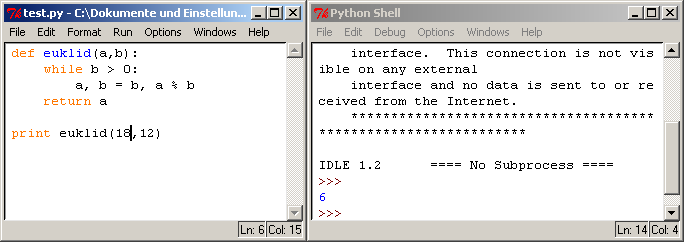
\includegraphics[scale=0.5]{graphics/IDLE.png}
	\caption{Python IDLE unter Windows}
	\label{fig:idle}
\end{figure}

Die Installation unter Linux ist ebenfalls einfach, denn entweder wird ein fertiges Packet der gew�hlten Linux-Distribution verwendet oder h�ndisch von den Sourcen kompiliert (\verb|configure, make, make install|). Unterschiedliche Python Versionen k�nnen in getrennten Verzeichnissen installiert und nebenl�ufig betrieben werden.

F�r Materialien, Dokumentation und Hilfestellungen ist die Python Website \cite{python:website} der erste Anlaufpunkt.

\item Ein speziell f�r Programmierneulinge zugeschnittenes Programm hat \cite{python:forkids} erarbeitet. Dessen zweite Auflage ist mit Ende 2006 gerade neu erschienen. Der Autor unterrichtet selbst an einem �sterreichischen Gymnasium und hat dieses Buch als Begleitbuch f�r den Einstieg in das Programmieren geschrieben. Anders als der Titel "'\textbf{Python f�r Kids}"' vermuten l�sst, ist die Lekt�re auch f�r �ltere Semester geeignet, sofern diese noch Programmierneulinge sind. Nat�rlich ist es auch als unterst�tzendes Lehrmaterial zu betrachten. 

\cite{python:forkids} hat f�r sein Buch ein eigenes Grafikmodul geschrieben. \textbf{xturtle} ist eine Erweiterung bzw. Verbesserung des \verb|turtle| Moduls. Die Idee des \verb|turtle| Moduls stammt aus der Programmiersprache Logo aus dem Jahre 1966, und ist ein Werkzeug f�r den Einf�hrungsunterricht in die Programmierung. Dabei wird eine programmierbare "'Schildkr�te"', die nach entsprechenden Befehlsvorgaben hin- und herlaufen kann, verwendet. Falls der Zeichenstift abgesenkt ist, zeichnet diese ihren zur�ckgelegten Weg auf (Abbildung \ref{fig:xturtle}).

\begin{quote}
{\itshape "'It's intended to be used in those educational situations, where an important requirement is easy access to graphics.
"'}\cite{python:forkids}
\end{quote}

Das \verb|turtle| Modul verwendet Tkinter\footnote{Tkinter: http://wiki.python.org/moin/TkInter} f�r die Darstellung von Grafiken und ist momentaner Bestandteil der Python Distribution. \verb|turtle| wird voraussichtlich mit Python 2.6 von \verb|xturtle| abgel�st\footnote{Diskussion: http://mail.python.org/pipermail/python-dev/2006-June/066677.html}.

\begin{figure}[h]
	\centering
	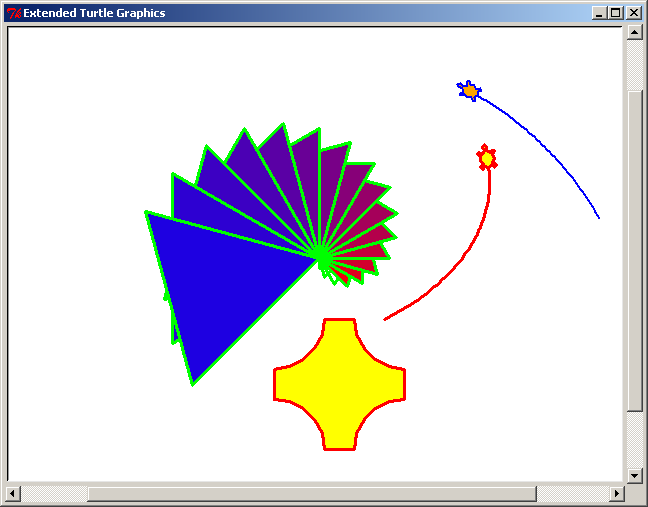
\includegraphics[scale=0.3]{graphics/xturtle.png}
	\caption{xturtle}
	\label{fig:xturtle}
\end{figure}

Auf der Website des Autors\footnote{weitere Materialien: http://ada.rg16.asn-wien.ac.at/~python/} finden sich zudem andere Unterrichtsmaterialien, wie z.B. Folien f�r den Einf�hrungsunterricht.

\item Wolfgang Urban arbeitet ebenfalls an einem �sterreichischen Gymnasium und stellt auf seiner Website\footnote{Wolfgang Urban: http://www.hib-wien.at/leute/wurban/} umfassendes Material f�r Mathematik, Physik und Informatikunterricht zur Verf�gung. Darunter implementiert er auch beispielhaft die Fibonacci-Folge in unterschiedlichen Variationen und mit verschiedenen Programmiersprachen. Mit diversen Sortieralgorithmen unter Python setzt er sich genauer auseinander.

\item "'\textbf{How to Think Like a Computer Scientist}"'\cite{python:thinkCS} ist ein Lehrbuch, das unter der \GNU\ Free Documentation License verf�gbar ist. Die Autoren haben dieses Buch w�hrend des Aufbaus ihres Curriculums verfasst und in weiterer Folge fortlaufend verbessert. Aufgrund des positiven Feedbacks aus aller Welt wurde das Buch f�r Java, Logo und C++ adaptiert. Eine zweite Version von \cite{python:thinkCS} ist derzeit in Arbeit und kann auf der Website des Projektes\footnote{Open Book Project: http://ibiblio.org/obp/thinkCS/python.php} eingesehen werden. Geplanter Fertigstellungstermin ist Anfang Juni 2007.

\item Materialien f�r fortgeschrittene Entwickler bietet Greg Wilson mit "'\textbf{Software Carpentry}"'\footnote{Software Carpentry: http://www.swc.scipy.org/}. Der Kurs richtet sich an Softwareentwickler, die schon praktische Erfahrung in Umgang mit Projekten gesammelt haben. Basis des Kurses ist Python. Das Thema ist die Wissenschaftlichkeit der Softwareentwicklung und die Vermittlung von Techniken, die das Arbeitsleben eines Entwicklers erleichtern sollen. Python wurde f�r diesen Kurs gew�hlt, um "'den zu vermittelnden Inhalten am wenigsten im Weg zu stehen"'. Das Material ist unter einer Open-Source Lizenz verf�gbar.

\item Die "'\textbf{Python Bibliotheca}"'\footnote{Python Bibliotheca: http://www.ibiblio.org/obp/pyBiblio/} ist eine Lehrplattform, die Tutorials, Workshops und Lehrmaterialien f�r den Unterricht mit Python bietet. Unter anderem ist ein Video\footnote{Video: "'A Python Love Story"': http://www.ibiblio.org/obp/pyBiblio/pythonvideo.php} mit Interviews bekannter Python-Gr��en, wie Guido van Rossum, zu finden.

\item \textbf{VPython}\footnote{VPython: http://vpython.org/} ist eine Sammlung von Python Klassen, die einen einfachen Zugang zu Echtzeit 3D Animationen erlaubt. Anwendungsbereich ist beispielsweise der Physikunterricht, wo das Arbeiten mit Vektoren oder physikalischen Abl�ufen wie Gravitation, visualisiert werden k�nnen (Abbildung \ref{fig:vpython}).

\begin{figure}[h]
	\centering
	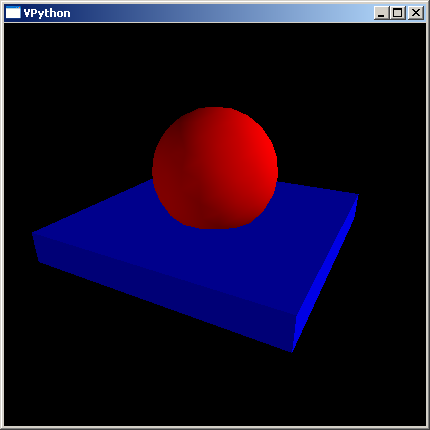
\includegraphics[scale=0.3]{graphics/vpython.png}
	\caption{Gravitationssimulation mit VPython}
	\label{fig:vpython}
\end{figure}

Auch das Visualisieren von Graphen ist mit VPython m�glich (Abbildung \ref{fig:vpython2}).

\begin{figure}[h]
	\centering
	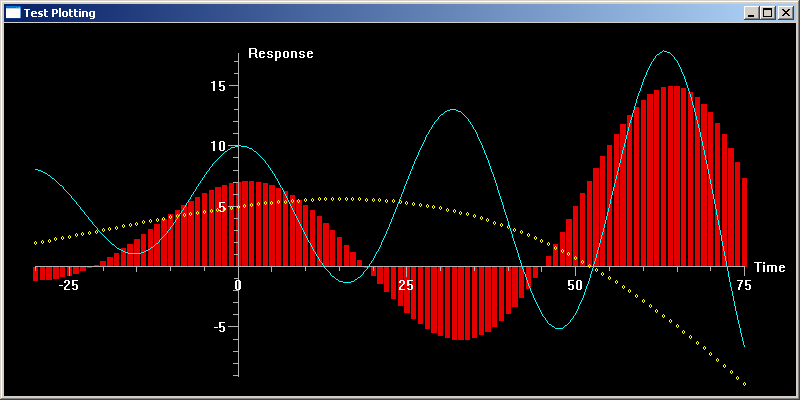
\includegraphics[scale=0.3]{graphics/graph-vpython.png}
	\caption{Darstellung eines Graphen mit VPython}
	\label{fig:vpython2}
\end{figure}

%\item PyNassi zu unwichtig

\item Mit \textbf{Tkinter}\footnote{Tkinter: http://wiki.python.org/moin/TkInter} und \textbf{wxPython}\footnote{wxPython: http://www.wxpython.org/} wird die \GUI\ Programmierung unter Python erm�glicht. Tkinter bedeutet \Tk\ Interface, ist also eine Schnittstelle zu \Tk\/, und \Tk\ ist eine \GUI\/-Bibliothek geschrieben in der Skriptsprache \Tcl\/ (man spricht dabei auch von Tcl/Tk\footnote{Tcl/Tk: http://tcl.sourceforge.net/}). Tkinter ist Bestandteil der Python-Standardbibliothek.
wxPython ist ein Wrapper um die C++-Bibliothek wxWidgets\footnote{wxWidgets: http://wxwidgets.org/}. 
Beide Module sind auf verschiedenen Betriebssystemen einsetzbar. Tkinter eignet sich vor wxWidgets durch die geringe Komplexit�t f�r den Einstieg in die GUI-Programmierung. wxPython skaliert besser und ist daher f�r die Entwicklung von komplexeren \GUI\/s geeignet.

\item \textbf{Gato}\footnote{Gato: http://gato.sourceforge.net/} erm�glicht die Visualisierung von Algorithmen auf Baumstrukturen (wie z.B. Suchbaumalgorithmen, k�rzester Weg, Kruskal oder Dijkstra). Das Tool wird auf der Universit�t K�ln entwickelt und bei Kursen �ber Algorithmen und diskrete Mathematik verwendet (Abbildung \ref{fig:Gato}). 

\begin{figure}[h]
	\centering
	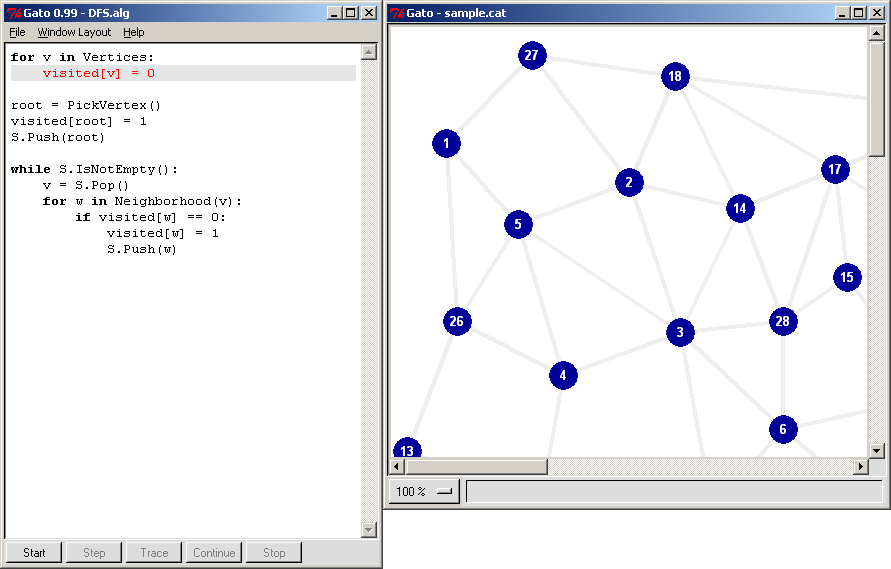
\includegraphics[scale=0.3]{graphics/gato.png}
	\caption{Gato}
	\label{fig:Gato}
\end{figure}

\item F�r die Entwicklung von Spielen gibt es eine Sammlung von Modulen, die unter \textbf{Pygame}\footnote{PyGame: http://www.pygame.org/} zusammengefasst sind. Pygame basiert auf der freien \SDL\/ - Bibliothek, die ein \API\ f�r Eingabe, Sound und Grafik zur Verf�gung stellt. Damit wird ein einfacher, high-level Zugang zur Spieleprogrammierung erm�glicht. % TODO Eine genauere Diskussion zur Spieleentwicklung im Unterricht ist unter Kapitel \ref{sec:firstlanguage} zu finden.

%\item Guido van Robot

\end{itemize}

%Zope f�r Webapllikations? (Djanfo turbogears?)
	
\newpage	
\section{Softwareentwicklung im Unterricht mit Zope}
\rkopf[]{Softwareentwicklung im Unterricht mit Zope}	
\label{sec:zope}
		
	\subsection{Komponentenarchitektur}
		%\subsection{CBSE - Komponentenbasierte Softwareentwicklung}
%Kurzes und b�ndiges Kapitel �ber CBSE, gerade soviel, um im  folgenden Kapitel auf die Unterschiede zu Zope 3 eingehen zu k�nnen.
%Hinweis auf die technisch komplexen Infrastrukturen der bekannten Komponententechnologien (CORBA, Java Beans, etc.) f�r den Unterrichtseinsatz. Erkl�rung der einfachen Inbetriebnahme eines Zope Servers.

%\subsection{Zope 3 vs. CBSE}
%Kann Zope 3 �berhaupt mit CBSE in Verbindung gebracht werden? Wie unterscheidet sich Zope 3 vom CBSE Ansatz? K�nnen CBSE Ideen anhand des Zope 3 Servers im Unterricht umgesetzt werden?
%Content (Model in MVC, Entity bean in J2EE)
%Views (View in MVC, Servlet in J2EE)
	
%Nicht-Fokus der beiden letzen Kapitel: zu starke Detaillierung in CBSE Richtung.

%%%%%%%%%%%%%%%%%%%%%%%%%%%%%%%%%%%%%%%%%%%%%%%%%%%%%

%Zope 3 bezeichnet sich selbst als Komponentensystem. Was zeichnet ein Komponentensystem aus? Was ist eine Komponente? Und warum ist ein Komponentensystem interessant f�r den Unterricht? Warum gerade Zope 3?

%Zope3 Komponenten Architektur
%	Was ist ein Komponentensystem? \cite{10.1109/CMPSAC.1996.544597}
%	Welche gibt es und wie funktionieren sie (grob)?
%	CBSE? WebServices?
%	Wichtigkeit der "Komponisierung"' der Softwareentwicklung? Ist die Softwarekomponente eine fundamentale Idee?
%	Einfacher Zugang zu einer Implementierung.
%	Zeigen was ist an Zope 3 das Komponentensystem, warum ists ein guter Einstieg/Ansatz?
%make or adapt (vs make or buy) 190.pdf

\Zope\ 3\footnote{Im Folgenden wird immer von Zope ab der Version 3 gesprochen. Ist die Rede von einer fr�heren Version, wird explizit die Versionsnummer angef�hrt.} besteht aus einer Komponentenarchitektur. Um diese zu erl�utern, soll zuerst der Begriff einer Softwarekomponente und der des \CBSE\ erl�utert werden.

In der heutigen Softwareentwicklung gibt es ein hohes Ma� an Anforderungen (modifiziert nach \cite{misc:goeschka_kos} und \cite{10.1109/CMPSAC.1996.544597}):
\begin{itemize}
	\item Hohe Qualit�t wird erwartet.
	\item Die Software muss billig sein.
	\item Usability: die Software mu� einfach und m�glichst ohne Lernaufwand zu bedienen sein.
	\item Neue Versionen und Updates werden in immer k�rzeren Zeitabst�nden verlangt. Auf �nderungen muss schnell reagiert werden.
	\item Stabilit�t, Zuverl�ssigkeit und Robustheit.
	\item Neue Software muss bestehende, alte Software integrieren und erweitern.
	\item Software wird immer komplexer.
	%\item Von Software h�ngen oft Menschenleben ab. %killed by alex ;)
\end{itemize}

Auf der anderen Seite erwartet man im Softwareentwicklungsprozess folgende Merkmale:
\begin{itemize}
	\item Die Erstellung der Software muss billig sein.
	\item Projektlaufzeiten m�ssen eingehalten werden.
	\item Prozess- und qualit�tsorientierte Entwicklung.
\end{itemize}

\cite{misc:goeschka_kos} schreibt weiters:

\begin{quote}
{\itshape "'Der Widerspruch aus den Kundenw�nschen und den Anforderungen an die Entwicklung f�hrt
fast zwangsl�ufig dazu, dass wir es heute als selbstverst�ndlich akzeptieren, dass Software
Fehler enth�lt. Wir wundern uns nicht mehr, wenn wir mehrmals am Tag unsere Systeme neu
booten m�ssen, weil sie komplett abgest�rzt sind (system crash). Den damit verbundenen
Verlust an wertvoller Arbeitszeit oder vielleicht sogar Datenverlust nehmen wir als
unerfreulich, aber allt�glich einfach so hin. W�rden wir uns bei einem Geb�ude oder einem
Auto auch so leicht zufrieden geben? Wohl kaum!"'}
\end{quote}

\CBSE\ soll dabei Abhilfe schaffen. Das Ziel komponentenbasierter Softwareentwicklung ist, die Produktivit�t und Qualit�t in der Softwareentwicklung zu steigern. Anstatt jedesmal "'das Rad neu zu erfinden"', soll Software aus Standardkomponenten "'zusammengebaut"' werden. Software soll nicht mehr entwickelt, sondern gekauft werden. Dabei spricht die Literatur von \COTS\ Komponenten.

\begin{quote}
{\itshape "'It [CBSE] focuses on reusing and adapting existing components, as opposed to just coding in a particular style.
CBSE encourages the composition of software systems, as opposed to programming them. CBSE is a process that aims to design and construct software systems using reusable software components."'}\cite{misc:cbsestuff}
\end{quote}

Ziel ist es, eine Industrialisierung der Softwareentwicklung zu erreichen. Damit w�rde die Softwareentwicklung zu einer klassischen Ingenieurswissenschaft mit einheitlichen Standards werden. Es g�be einen eigenen Markt f�r den Handel mit Komponenten (Abbildung \ref{fig:componentmarket}). 

\begin{figure}[ht]
	\centering
	
\includegraphics[scale=0.8]{graphics/componentmarket.png}
	\caption{Beispiel eines Komponentenmarktes nach \cite{10.1109/CMPSAC.1996.544597}}
	\label{fig:componentmarket}
\end{figure}

Ein hochgestecktes Ziel, wenn man die rasante technologische Entwicklung betrachtet. Kaum werden Vorschl�ge ausgearbeitet, sind sie auch schon wieder veraltet. Die Herausforderung besteht darin, die Thematik frei nach dem Horizontalkriterium der fundamentalen Idee nach Schwill zu bearbeiten. Wie k�nnen Standards geschaffen werden, die m�glichst frei von Technologie, aber trotzdem mit jeder Technologie eingehalten werden k�nnen? Und wie kann es in der kommerziellen Welt der Konkurrenz zu \emph{einer} einheitlichen L�sung, also zu einem Standard, kommen?

Dazu kommen noch die Akzeptanzschwierigkeiten bei vielen Entwicklern, die ihre Arbeit als kreativen Prozess sehen und sich durch die �berstrukturierung von Prozessen bedr�ngt f�hlen. \cite{misc:componentssmalltalk} sieht die Softwareentwicklung sogar als eine Kunst und bekr�ftigt unter anderem Folgendes:

\begin{quote}
{\itshape "'Bedenkt man, da� der Computer eine universelle Maschine ist und Software praktisch beliebige Vorg�nge beschreiben kann, wird klar, dass der Ansatz eines universellen Vorgehensmodells zum Scheitern verurteilt ist."'}
\end{quote}

\cite{misc:componentssmalltalk} unterteilt Softwareentwicklung, unter Berufung auf andere Quellen, in zwei unterschiedliche Kulturen, die griechische und die r�mische Kultur. Wobei zur kurzen Erl�uterung hier die Schubladen \emph{Entwickler} und \emph{Manager} zu verstehen sind. Wenngleich sehr �berspitzt formuliert, erl�utert diese Aufteilung eine weitere Problematik, die das Finden einer gemeinsamen und akzeptierten Ingenieurswissenschaft erschwert.

Spinnt man den Faden weiter, kann eine Verbindung zur unterschiedlichen Weltanschauung von Open-Source Software und kommerzieller Closed-Source Software gesehen werden. \CBSE\ geht laut Literatur davon aus, dass Komponenten als \emph{Blackbox} ausgeliefert werden. Das hei�t, der Kunde kennt die Implementierung nicht, nur die Schnittstellendefinition. Dieser Ansatz widerspricht zutiefst der Open-Source Philosophie. \CBSE\ kann jedoch nur funktionieren, wenn der Kunde die Implementierung der Komponente nicht ver�ndern kann, andererseits w�re die Idee fehlerfreier Software wieder hinf�llig. Der Hersteller kann nur f�r \emph{sein} Produkt garantieren, das er mit seinem Spezialwissen qualitativ hochwertig h�lt. �ndert der Kunde etwas an der Komponente, erlischt die Garantie und Fehlern sind wieder T�r und Tor ge�ffnet. Eine m�gliche Abhilfe w�re die Auslieferung von Komponenten als \emph{glass-box} \cite{misc:reuse}, wobei der Quelltext der Komponenten mit ausgeliefert wird, dieser jedoch nicht ver�ndert werden darf.

Diese Arbeit will und kann hier keine L�sung erarbeiten. Die bisherige Abhandlung zeigt, dass \CBSE\ uns die n�chsten Jahre begleiten wird, und das Thema Modularisierung, Reuse und Testen von Software einen wichtigen Platz in der Ausbildung angehender Softwareentwickler einnehmen mu�.

Was ist nun eigentlich eine Komponente? \cite{misc:reuse} hat die unterschiedlichen Definitionen aus der Literatur zusammengefasst und folgende Merkmale abgeleitet:
\begin{itemize}
	\item Komponenten sind klar abgrenzbar: sie k�nnen unabh�ngig entwickelt und eingesetzt werden.
	\item Sie stellen Schnittstellen nach au�en zur Verf�gung und kapseln ihre Daten.
	\item Sie haben definierte Abh�ngigkeiten von ihrem Kontext.
\end{itemize}

Eine nach \cite{misc:komponentenmodelle} allgemein anerkannte Definition einer Komponente ist:

\begin{quote}
{\itshape "'A software component is a unit of composition with contractually specified interfaces and explicit context dependencies only. A software component can be deployed independently and is subject to composition by third parties."'}
\end{quote}

Wenden wir uns jetzt der Komponentenarchitektur von \Zope\ zu. Die \Zope\ Komponentenarchitektur kann nicht im globalen Umfeld einer \CBSE\ Komponente gesehen werden. Eine Komponente unter \Zope\ ist eine Stufe davor anzusiedeln, n�mlich in der Entwicklung selbst. \Zope\ selbst ist ein Applikationsserver, der auf einer Komponentenarchitektur (\verb|zope.component|, \verb|zope.interface|) und weiteren Komponenten basiert. Diese \emph{core} Komponenten k�nnen durch die Komponentenarchitektur flexibel angepasst und erweitert werden, ohne die originale Funktionalit�t zu ver�ndern.

Passend dazu definiert \cite{misc:reuse} drei Typen von Komponenten unterschiedlicher Granularit�t: Elementarbausteine, Baugruppen und Systeme.

\begin{quote}
{\itshape "'Elementarbausteine sind der kleinste Komponententyp. Sie haben beliebige
Abh�ngigkeiten von anderen Komponenten und sind nicht f�r sich ausf�hrbar [...]
Baugruppen sind Komponenten mittlerer Gr��e. Sie bestehen aus Elementarbausteinen
und/oder anderen Baugruppen. Sie haben klar begrenzte Abh�ngigkeiten
von anderen Komponenten und sind nicht f�r sich ausf�hrbar. [...]
Systeme sind die gr��ten Komponenten. Sie sind aus Baugruppen zusammengesetzt,
haben minimale Abh�ngigkeiten von anderen Komponenten und sind
f�r sich ausf�hrbar."'}
\end{quote}

Eine \Zope\ Komponente ist als Baugruppe einzustufen, w�hrend die Komponente, von der \CBSE\ spricht, eher dem System  zuzuordnen ist. Die \Zope\ Komponentenarchitektur ist im Prinzip ein Entwicklerwerkzeug zum Software Reuse, das den gleichen Merkmalen, wie bei \cite{misc:reuse} dargelegt, unterliegt. Einziger Unterschied ist, dass die \Zope\ Komponente nicht ausgeliefert und \emph{deployed}, sondern f�r die Entwicklung einer Applikation\footnote{Unter Zope typischerweise eine Webapplikation.} verwendet wird. Diese Applikation kann theoretisch als Komponente nach \CBSE\ verwendet werden. 

\Zope\ selbst hat keine komplexe Verteilungstechnologie wie z.B. \EJB\ mit \RMI\ hat. \Zope\ kann per Standard mit XML-\RPC\ umgehen\footnote{Die Zope Community hat bisher keinen Bedarf in der Integration aufwendigerer Technologien gesehen.}. Daf�r ist es m�glich, auf verteilte Konzepte wie \CORBA\ oder Webservices zu setzen. F�r Python exisitieren mehrere \ORB\/\footnote{z.B. omniORB: http://omniorb.sourceforge.net/}, und f�r den \Zope\ Server gibt es eine experimentelle Komponente f�r das \SOAP\/\footnote{http://svn.zope.org/soap/}.

Auch wenn die Zope Archtitekur aus den genannten Gr�nden nicht der Idee des \CBSE\ entspricht, verfolgt sie doch den Komponentengedanken und ist, nach Ansicht des Autors, f�r die Vermittlung der Thematik im praktischen Bezug gut im Unterricht anwendbar. Der Einsatz von Python wurde im ersten Abschnitt dieser Arbeit behandelt. Ist den Studenten die Sprache gel�ufig, geht es im Unterricht nur noch um das Erlernen neuer Konzepte. Die Anwendung erfolgt mit gewohntem Werkzeug.

Das modulare Komponentendenken ist eine fundamentale Idee der Softwareentwicklung und geh�rt vermittelt. Der Autor kennt neben Zope kein anderes Framework, das ohne in die Komplexit�t von verteilter Software einzutauchen, diese Thematik leicht zug�nglich macht.

%TODO? 5. mehr details? Komponentenarchitektur unter Zope 3
%TODO? 6. Eggs vs komponentenmarkt



	
	\subsection{ZODB}
		\label{sec:ZODB}
		Wie in Kapitel \ref{sec:Grundlagen_Zope} schon erw�hnt, wird \Zope\ mit der \ZODB\ ausgeliefert. Die \ZODB\ ist f�r die Persistierung der Pythonobjekte zust�ndig. Damit die in der Applikation verwendeten Objekte bei einem Neustart des \Zope\ Servers nicht verloren gehen, werden diese Objekte persistiert.
	
\ZODB\ arbeitet mit dem \verb|pickle|\footnote{pickle: http://docs.python.org/lib/module-pickle.html} Modul, um Objekte schreiben und lesen zu k�nnen. Daten werden dabei von komplexen Objekten in einen Bytestream umgewandelt. Dieser kann nun z.B. in einem File gespeichert werden. 
	
\begin{lstlisting}[style=interpreter]
>>> pickle.dump(object, file)
\end{lstlisting}
	
Um aus einem Bytestream wieder ein Objekt zu erhalten, ist ebenfalls nur eine Zeile Quelltext notwendig.
	
\begin{lstlisting}[style=interpreter]
>>> object = pickle.load(file)
\end{lstlisting}

Man spricht dabei von \emph{pickling} (Serialisierung) und \emph{unpickling} (Deserialisierung). Die \ZODB\ k�mmert sich um die gesamte Maschinerie: Caching, Schreiben und Lesen. Das Ganze ist nat�rlich transaktionssicher\footnote{siehe Maillinglisteneintrag "'ZODB implementiert kein ACID"': https://mail.dzug.org/pipermail/zope/2007-June/003937.html}. Um ein Objekt zu persistieren reicht eine simple Vererbung.

\begin{lstlisting}[style=interpreter]
>>> from persistent import Persistent
>>> class MyPersistentClass(Persistent):
...		def __init__(self):
...			self.id = ''
...			self.name = ''
...			self.description = ''
...
\end{lstlisting}
	
Als Standard schreibt die \ZODB\ in ein File im Dateisystem. Diese Implementierung wird "'FileStorage"' genannt. Es ist m�glich, auf andere Implementierungen zuzugreifen. Diese sind "'DirectoryStorage"'\footnote{DirectoryStorage: http://dirstorage.sourceforge.net/}, "'ClientStorage"' und "'\APE\/"'\footnote{APE: http://hathawaymix.org/Software/Ape}.

Aus diesen Alternativen ist die "'ClientStorage"' erw�hnenswert, mit der Daten mittels \ZEO\ auf mehrere Rechner verteilt werden. Damit ist Clustering von Webapplikationen allein auf Basis kostenloser Open-Source-Software m�glich \cite{zope:ctarticle1}.

Wie kann die \ZODB\ nun im Unterricht verwendet werden? Es ist sinnvoll, im Zuge der Verwendung von \Zope\ in einigen wenigen Unterrichtseinheiten auf das Thema einzugehen. Dabei sollte jedoch nicht zu sehr ins Detail gegangen werden. Es bietet sich an, die ZODB zur Veranschaulichung der unterschiedlichen Handhabung von objektorientierten und relationalen Datenbanken zu zeigen. 

\begin{quote}
{\itshape "'An advantage of relational database systems is their programming-language neutrality. Data are stored in tables, which are language independent. An application must read data from tables into program variables before use and must write modified data back to tables when necessary. This puts a significant burden on the application developer. A significant amount of application logic is devoted to translation of data to and from the relational model."'}\cite{python:fulton}
\end{quote}

Bei relationalen Datenbanken wird, unabh�ngig von der Implementierung mittels \SQL\/, auf die Daten zugegriffen und diese mit der Applikation verwoben. Dabei ensteht ein nicht unerheblicher Aufwand f�r den Entwickler, der sich um die Handhabung der Daten selbst k�mmern muss.

\begin{quote}
{\itshape "'An alternative is to retain the tabular structure in the program. For example, rather than populating objects from tables, simply create and use table objects within the application. In this case, high-level tools can be used to load tables from the relational database. With sufficient knowledge of database keys, tools could automate saving data when tables are changed. A disadvantage of this approach is that it forces the application to be written to the relational model, rather than in an object-oriented fashion. The benefits of object orientation, such as encapsulation and association of logic with data are lost [...] Object databases provide a tighter integration between an applications object model and data storage. Data are not stored in tables, but in ways that reflect the organization of the information in the problem domain. Application developers are freed from writing logic for moving data to and from storage."'}
\end{quote}

\cite{python:fulton} schreibt hier von zwei Varianten. Die eine ist eine Hybridl�sung, n�mlich das Objektmapping. Hierbei werden die Daten in der Applikation verwendet, die notwendigen Abfragen an die relationale Datenbank geschehen im Hintergrund. Hier ist der Entwickler jedoch zu stark an das relationale Denken gebunden. 

Die zweite Variante ist das Verwenden einer objektorientierten Datenbank, wie die \ZODB\/. Hierbei r�cken Daten und Integration n�her zueinander, ohne jedoch problematisch zu verschmelzen. Die Entwicklung muss sich nicht um das Speichern und Lesen von Daten k�mmern.

In Verbindung mit der ersten Variante soll SQLAlchemy\footnote{SQLAlchemy: http://www.sqlalchemy.org/} erw�hnt werden, ein Python SQL Toolkit und objektrelationaler Mapper. SQLAlchemy kann als Hibernate\footnote{Hibernate: http://www.hibernate.org/} der Pythonwelt betrachtet werden. Die folgende Interpreter Session zeigt stark verk�rzt die Anwendung eines Objektmappers, wo gegen Ende zu sehen ist, wie der Mapper eine \SQL\/-Abfrage im Hintergrund absetzt.

\begin{lstlisting}[style=interpreter]
>>> class User(object):
...		def __init__(self, username, password):
...			self.userid = None
...			self.username = username
...			self.password = password
...		def get_name(self):
...			return self.username
...		def __repr__(self):
...			return "User id %s name %s password %s" % (repr(self.userid), \
...								repr(self.username), repr(self.password))
...
>>> mapper(User, users_table)
>>> sess = create_session()
>>> user = User('hak', 'tom')
>>> sess.save(user)
>>> sess.flush()
INSERT INTO users (username, password) VALUES (:username, :password)
{'password': 'hak', 'username': 'tom'}
>>> user
User id 1 name 'hak' password 'tom'
\end{lstlisting}




		
  \subsection{Softwareentwicklungsprozess erleben}
  	%Paper �ber Zope(2) Projekt an schule: http://tech.canterburyschool.org/tech/PyCon04Paper
%naja nicht so geeignet.

%Anhand einer Implementierung kann man Studenten in Form eines kleinen Projektes den professionellen Softwareentwicklungsprozess erleben lassen. Wichtigkeit der Versionierung (Nachvollziehbarkeit) jeder Implementierung hervorheben. Heutzutage kommt man ohne Code-Repository und sinnvolle Teststrategie in der Implementierung nicht weit. Die Rahmenbedingungen hierf�r werden in diesem Kapitel behandelt.

Anhand einer Implementierung kann man Studenten in Form eines Projekts den professionellen Softwareentwicklungsprozess erleben lassen. Was ist dabei zu beachten? Wie kann der Unterricht gestaltet werden? Was sollten die Studenten daraus mitnehmen? Die letzte Frage erl�utert \cite{misc:803190} schon im Jahre 1978. Ein Student sollte nach Abschluss der Lehrveranstaltung folgende Kenntnisse besitzen:

\begin{quote}
{\itshape 
	\begin{itemize}
		\item "'Do Software Development by accurately using at least one state-of-the-art method in each of the four major areas of analysis, design, implementation, and testing;
		\item Test and Measure software by devising and carrying out well-designed experiments that will validate a software system's quality (e.g., reliability, efficiency) and that will identify any parts of the system needing work;
		\item Manage effectively a moderate sized project (3-7 people for 1-2 years)
		\item Communicate effectively with users, managers, and other technical people;
		\item Learn new software engineering methods rapidly, and be able to keep up with relevant advances in computer science."'
	\end{itemize}
}
\end{quote}

Wenngleich die zitierte Literatur schon veraltet erscheint, kann sie doch auf erstaunlich pr�zise Art vermitteln, was bei der Gestaltung einer solchen Lehrveranstaltung wichtig ist: 

\begin{itemize}
	\item Methodik und Werkzeuge (z.B. Testen)
	\item Kommunikation, Projektmanagement
	\item Motivation bzw. Wecken des Forschergeistes
\end{itemize}
%TODO eingehen auf die Punkte?
Das Schl�sselwort, mit dem alle diese Ziele erreicht werden k�nnen, hei�t \emph{Praxisbezug}. \cite{misc:swe} hat untersucht, unter welchen Kriterien Studenten eine Lehrveranstaltung als praxisnahe empfinden (vgl. Sinnkriterium der fundamentalen Idee nach \cite{schwill1}):

\begin{description}
	\item[Lernhandeln] Die Veranstaltung bietet viel Freiraum f�r den eigenen Beitrag.
	\item[�berraschungseffekt] Die Lehrveranstaltung bietet ein neues oder im Ausbildungskontext �berraschendes Erlebnis f�r die Teilnehmer.
	\item[Authentizit�t und Nutzen] Die jeweiligen Lehrinhalte sind f�r die Studenten nachvollziehbar praxisrelevant. Authentizit�t entsteht insbesonders, wenn der Lektor �ber eigene Praxiserfahrung verf�gt und �ber diese berichten kann. Letzthin kommt man um die Erkenntnis nicht herum, dass nur solche Personen Software Engineering authentisch und praxisnahe unterrichten k�nnen, die selbst in der Praxis Software Engineering betrieben haben oder betreiben.
\end{description}

\cite{misc:swe} z�hlt M�glichkeiten auf, Praxisn�he im Unterricht zu vermitteln.

\begin{description}
	\item[Echte Kunden, echte Anwendung] F�r Praxisn�he spricht nat�rlich ein Beispiel aus der Praxis. Studenten profitieren von echten Kunden mit echten Anwendungen. Wobei es kaum m�glich ist, im Hochschulbetrieb mit kommerziellen Kunden im Unterricht umzugehen. Es gibt jedoch Erfolge mit Non-Profit-Organisationen. Die Schwierigkeit besteht darin, Jahr f�r Jahr Kunden vom ihrem gewonnenen Mehrwert zu �berzeugen. Ein Argument daf�r w�re Networking mit den Studenten. Begabte Studenten k�nnen quasi "'gescoutet"' werden. Die Hauptaufgabe des Lektors sollte die Gestaltung des Curriculums sein. Dieser w�re aber mit der j�hrlichen Kooperation mit realen Kunden �berfordert. Abhilfe k�nnte hier eine Unterst�tzung von Seiten des Unterrichtsministeriums sein, z.B. mit F�rderungen f�r kooperationswillige Firmen bzw. Schaffen von Strukturen f�r die Abwicklung solcher Lehrveranstaltungen. Momentan ist es eher �blich, den Kunden selbst in einer Art Rollenspiel zu vertreten. Dabei treten aber Glaubw�rdigkeits- und Akzeptanzprobleme auf.
	\item[Kundengespr�che] Eng mit dem ersten Punkt dieser Aufz�hlung verkn�pft, sind die Kundengespr�che. Dabei k�nnen parallel dazu gleich professionelle Gespr�chsstrategien gelehrt werden. Die Studenten lernen aus den Informationen des Kunden das Essentielle herauszufiltern. Das Projektteam muss geschlossen, aber mit f�r den Kunden �bersichtlicher Struktur auftreten. Hierbei k�nnen auch Gespr�che mit unterschiedlichen Kundengruppen trainiert werden, beispielsweise ein Meeting mit der technischen Abteilung oder mit dem Gesch�ftsf�hrer selbst. Letzteres wird bei tats�chlichen Kunden wohl eher unrealistisch sein.
	\item[Professionalit�t in der Form] Das korrekte Erbringen z.B. eines Angebotes, ist nicht nur in inhaltlicher Form, sondern auch als Erscheinungsbild in der Praxis wichtig. Ergebnisse m�ssen �bersichtlich, und f�r den Kunden ersichtlich, die relevante Botschaft �bermitteln.
	\item[Kundenorientiertes Denken] Was dem Team wichtig ist, ist meist klar. Doch was ist dem Kunden wichtig? Aus den Gespr�chen soll hier eine Abstrahierung stattfinden. Das Projekteam, das wohl eher technisch denken wird, muss sich hier in die Denkweise des Kunden hineinversetzen und diese verstehen. Danach m�ssen die Studenten diese Erkenntnis mit ihren Zielen oder Vorgaben abstimmen und daraus einen Kompromiss schlie�en. Einerseit muss der Kunde befriedigt werden, aber der Spa� an der Arbeit darf nicht verloren gehen!
	\item[Komplexere Projekte und Reverse Engineering] Beim Reverse Engineering wird eine bestehende Software analysiert und rekonstruiert bzw. erweitert oder verbessert.
	\begin{quote}
	{\itshape "'Programming from scratch: Most courses teach students to code from scratch, rather than by modifying existing programs or by working from model solutions. Moreover, students rarely read good programs. It's as if we asked students to write good prose without first reading good prose [..] Modify and combine programs as well as creating them. Teach students to work with program structures devised by others, to reuse components, to adhere to standards, and to value good documentation."'}\cite{336592}
	\end{quote}
	
	Nicht nur das Erstellen einer Software von Beginn an, sondern auch das Weiterverwenden und Verbessern existierender Software sollte einem Studenten vermittelt werden. Gute Software kann analysiert und Beispielen schlechter Software gegen�bergestellt werden. Nat�rlich fehlt in einem Semester die Zeit f�r ein gro�es Softwareprojekt. Eine M�glichkeit besteht jedoch darin, das Projekt �ber eine l�ngere Laufzeit zu planen und das Projektteam (die Studenten) immer wechseln zu lassen. Hier bleibt die Frage offen, wie �berschaubar und kontrollierbar dieser Ablauf f�r den Lektor w�re. \cite{misc:reverseengineering} beschreibt die Erfahrungen bei der Durchf�hrung eines Reverse-Engineering Projekts im Hochschulbetrieb:
	
	\begin{quote}
	{\itshape "'[...] bieten gerade Projekte, die auf existierender Software aufbauen eher praxisorientierte
Bedingungen. Sie sind �konomischer, da sie den Aufwand, der in existierender
Software steckt (Implementations- und Testaufwand), nachnutzen. Damit ist die Bew�ltigung
komplexer Software auch unter Hochschulbedingungen m�glich."'}
	\end{quote}
	
	Und hier kommt \Zope\ wieder ins Spiel. Eine Neuentwicklung ist ebenso m�glich, wie Reverse Engineering einer bestehenden Software. Weiters kann \Zope\ selbst analysiert werden, um die internen Funktionalit�ten und Abl�ufe besser zu verstehen. Oder besser gesagt, um zu lernen, wie spezifische Problemstellungen von anderen Softwareentwicklern umgesetzt werden.
	
	\item[Harte Termine] Die gestellte Aufgabe muss zu einem festgelegten Termin erf�llt werden. Der Termin sollte so gew�hlt werden, dass sich mit durchschnittlichem Aufwand der Gesamt- oder Teilprojektumfang nicht realisieren lassen w�rde. So m�ssen die Studenten Abstriche (Mehrarbeit, Qualit�ts- oder Funktionalit�tseinbu�en,...) machen, um die Deadline halten zu k�nnen. Die daraus entstanden Konsequenzen werden diskutiert und m�ssen auch vor dem Kunden glaubhaft gerechtfertigt werden k�nnen.
	\item[Professioneller Werkzeugeeinsatz] Arbeitsweise, Werkzeuge und Frameworks, die in der Industrie Verwendung finden, f�rdern das Verst�ndnis der Praxisrelevanz bei den Studenten. Wobei hier wiederum das Hauptaugenmerk mehr auf die fundamentalen Konzepte zu legen ist, als auf Modeerscheinungen. Das zu erkennen,  erfordert ein hohes Ma� an Wissen und Erfahrung in der entsprechenden Materie. Somit sollte keine Spezialisierung auf ein Framework oder Tool stattfinden, sondern dieses als Werkzeug zum Curriculum betrachtet werden, dessen Inhalte es zu lehren gilt. \Zope\ bietet, neben einfacher Installation und Wartung im Universit�tsbetrieb, den Zugang zu komplexerer softwaredidaktischer Thematik, ohne sich zu stark auf das Framework zu spezialisieren. Die Infrastruktur kann also einfach eingerichtet und jedem Studenten, auch f�r den privaten Gebrauch zu Hause, verf�gbar gemacht werden.
	\item["'Dirty Tricks"'] \cite{misc:swe} schreibt, dass k�nstlich herbeigef�hrte Serverabst�rze, korrupte Code Repositories usw. helfen, realit�tsnahen Praxisbezug herzustellen. Diese Methode erscheint fast geh�ssig, zumal die Studenten sicher genug mit eigenen Problemen innerhalb des Projekts zu tun haben. Trotzdem ist eine Reflexion der erlebten Komplikationen sowohl technischer als auch sozialer Natur sicherlich lehrreich.
\end{description}

%\textbf{Verteiltes Wissen}
%Erfolg im Umgang mit Unterschiedlichen Vorkenntnissen

Da der Fokus eines solchen Projekts nicht prim�r auf der Programmierung liegt, sollten die notwendigen Kenntnisse schon vermittelt worden sein. Wird der Lektor trotzdem mit unterschiedlichen Wissensst�nden der Studenten konfrontiert, muss diesen der klare Mehraufwand kommuniziert werden. Eventuell m�ssen sich die Betroffenen eine Einf�hrung in die Programmierung selbst erarbeiten, wenn das notwendig erscheint. Bei einer Sprache wie Python wird das nat�rlich um ein Vielfaches erleichtert, wie ab Kapitel \ref{sec:firstlanguage} ausf�hrlich diskutiert wurde. Trotzdem sollte beachtet werden, dass Studenten mit Erfahrung in der Programmierung bestimmt mehr aus dem Projekt mitnehmen, da sie sich durch ihr vorhandes Wissen, vollst�ndig auf das Erlernen von Methodik und Werkzeugen konzentrieren k�nnen.

Die Aufgaben in der Projektarbeit k�nnen nat�rlich je nach F�higkeiten der Studenten unterschiedlich verteilt werden, jedoch mu� darauf geachtet werden, dass keine "'Trittbrettfahrer"' mitgeschleppt werden. Ein weiteres Hilfsmittel zur Wissensverteilung bei unterschiedlichem Know-how in Projektgruppen ist das Pair-Programming aus dem \XP\/ \cite{318762}, einem Vorgehensmodell in der Softwarentwicklung. Dabei sitzen immer zwei Studenten gemeinsam vor einem Bildschirm, um eine Aufgabe zu l�sen. Einer von beiden kontrolliert die Eingabeger�te, der andere sieht �ber die Schulter, schl�gt Fragen nach oder dokumentiert die momentanen Arbeitsschritte.

\begin{quote}
{\itshape "'Our experiments and experiences with pair-programming in the computer science classroom have been favorable. Ultimately, students are able to complete programming assignments faster and with higher quality. Students communicate with each other more, appear to learn faster, and are happier and less frustrated. The temptation to cheat is greatly reduced. Additionally, the workload of the educators is reduced."'}\cite{364614}
\end{quote}

Zahlreiche Studien, wie \cite{563353}, \cite{misc:xpstuff} belegen den positiven Effekt von Pair-Programming im Unterrichtseinsatz.

%-Teile aus XP vostellen! Coderepos, Pair Programming, Testing

%Soft-skills, nach sdm_pub

%-Design - implementierung - test
%-Software Life Cycle

%Lernen von der Community
%Opensource

Der Autor kann die Erkenntnisse aus der Literatur best�tigen, da er selbst an der \FH\ Technikum Wien, im Zuge der Spezialisierungsveranstaltung Informationsmanagement, mit sechs weiteren Studenten in ein Projekt involviert war.
Vision des Projekts war ein einfach bedienbares, web-basiertes Projektmanagement-Tool, realisiert mit dem Fokus auf offene Standards.

Das Projekt gliederte sich in zwei Phasen: das Vorprojekt und das Hauptprojekt. Die Projektdauer betrug zwei Semester. Im Zuge des Vorprojekts wurden vor allem eine umfangreiche Marktstudie durchgef�hrt, die anwendbare Technik evaluiert, die erw�nschten Anforderungen spezifiziert und ein Pflichtenheft erstellt. Dieses stellte die Grundlage f�r die Aufgaben im Hauptprojekt dar. Auch wurde das Vorprojekt selbst projektmanagementorientiert durchgef�hrt und dahingehend genutzt, einiges �ber Abl�ufe und Probleme in einem konkreten Projekt zu erfahren.

Im Vorprojekt, der Analysephase des Gesamtprojekts, wurde mit einem Unternehmen kooperiert, welches Interesse am eventuell entstehenden Produkt �u�erte. Bei einem Meeting in den R�umlichkeiten der Firma wurde die Produktidee pr�sentiert und Feedback eingeholt. Die Praxisrelevanz war f�r das Team kein Thema, sie war offensichtlich vorhanden. Die Motivation war dementsprechend in hohem Ma�e gegeben. In dieser Phase wurde, bis auf einen Mini-Prototypen, nichts entwickelt. Die Arbeit wurde haupts�chlich auf die Vorgehensweise in der Analysephase, die Kommunikation und Abstimmung im Team und das Projektmanagement fokusiert. Die Probleme, die dabei auftraten, waren sehr lehrreich, obwohl alle involvierten Studenten nebenher berufst�tig waren und somit dementsprechende Erfahrungen schon gesammelt hatten.

Aus den Erfahrungen des Vorprojekts wurde f�r das Hauptprojekt die Erstellung eines Prototypen f�r ein Projektmanagementtool mit zwei integrierten lokalen Diensten und einem integrierten externen Dienst, sowie der Entwurf und die Realisierung einer Schnittstelle nach au�en als Projektziel definiert. Die urspr�ngliche Idee, eine fertige Software zu entwickeln, wurde aus Komplexit�tsgr�nden, die sich erst im Verlauf der Analysephase ergaben, eingestellt. Selbst die Entwicklung eines Webservice-orientierten Prototypen geriet unter Zeitdruck, und so wurde die Funktionalit�t der \GUI\ stark minimiert.

Im Hauptprojekt wurde prim�r entwickelt. Das Team bestand aber nur aus zwei berufst�tigen Entwicklern, weshalb die Wissensverteilung nicht homogen war. Durch den Einsatz von Pair-Programming konnte der Wissensstand insofern angeglichen werden, als eine sinnvolle Teameinteilung und Entwicklung m�glich wurde.

Mit Ende der zwei Semester und mit Abschluss der Lehrveranstaltung wurde die Entwicklung des Prototypen fertiggestellt. Es w�re durchaus interessant, diesen Prototypen in den nachfolgenden Semestern zu behandeln. Kann der Prototyp weiterentwickelt oder verbessert werden? Welche Fehler wurden bei der Entwicklung gemacht? Eventuell kann die gleiche Funktionalit�t auf Basis einer anderen Technologie implementiert werden. M�glichkeiten g�be es viele. Die Frage ist jedoch, welche Studentengruppe motiviert w�re, sich genau mit dieser Thematik auseinanderzusetzen, denn wie schon weiter oben beschrieben, ist die Motivation f�r den Lerneffekt wichtig.
  	
  \subsection{Testen und Dokumentieren von Software}
  	%Testen und Dokumentieren wird wie ein Stiefkind behandelt. Warum ist es sinnvoll, diese Themen im Informatikunterricht st�rker hervorzustreichen? Mit Zope 3 ist dieser Ansatz sehr sch�n zu realisieren, da er vom Framework und der Art der Implementierung unterst�tzt wird.
Testen und Dokumentieren von Software gewinnt erst bei gro�en Softwareprojekten an Relevanz. Dementsprechend wird das Testen von Software im Unterricht vernachl�ssigt, da nur in seltenen F�llen gro�e Projekte realisiert werden, bei denen das Testen unerl�sslich wird. 
Bei kleinen Projekten ist es auch schwer, den doch enormen Aufwand vor den Studenten zu rechtfertigen. Die Fehler scheinen bei normaler Benutzung der Software viel schneller gefunden zu werden.

Selbst in der Industrie scheint es, als ob das Testen von Software nicht durchg�ngig als wichtiges Element im Softwareentwicklungsprozess gesehen wird. Eine Studie aus dem Jahr 2003 \cite{misc:testingsurvey} besagt, dass 52\% der befragten Softwareentwickler ihren Code testen, 34\% manchmal und 14\% �berhaupt nicht. Testen wird als l�stiges und langweiliges Anh�ngsel gesehen. Hier ist ein deutlicher Nachholbedarf ersichtlich. Nach Erfahrung des Autors ist das nur theoretisch in die Lehre vorgedrungen, die praktische Anwendung kommt jedoch zu kurz.

\begin{quote}
{\itshape "'Developers reuse code but do not test it to the
extent we expected [...] simple to use tools are lacking when it comes to test creation and test analysis [...] knowledge on the importance of testing in general and \emph{unit} testing in particular seem low"'}\cite{misc:testingsurvey}
\end{quote}

Entwickler testen so gut wie keine Reuse-Implementierung. Gerade bei der Zunahme an Reuse und der Komponentenorientierung von Software verlagert sich die Relevanz von der Entwicklung zum Testen. Die Komponenten selbst m�ssen mit Tests ausgeliefert werden, und die Benutzung dieser erfordert weitere Integrationstests. Weiters werden Tools zur Erstellung und Validierung von Tests als unbefriedigend empfunden. Die Wichtigkeit der Thematik wird generell untersch�tzt.

Im Folgenden werden die unterschiedlichen Testm�glichkeiten mit \Zope\ besprochen. Eine tats�chliche Umsetzung davon wird in der Beispielimplementierung, Kapitel \ref{kapitel:Beispielimplementierung} pr�sentiert. Weiters wird auf das \emph{doctesting}, einer Testmethode mit gleichzeitiger Dokumentation eingegangen.
  
\paragraph*{Unit Tests}

Ein \emph{Unit test} ist ein White-Box Test, wobei nur eine spezielle Komponente f�r sich allein getestet wird. Der Test wird von der Umwelt (wie andere Komponenten) nicht beeinflusst. Er testet die kleinste �berhaupt testbare Einheit (Unit) einer Software. Ziel ist die Funktionalit�t jeder einzelnen Komponente zu garantieren. Nach dem \TDD\/ \cite{952753} werden \emph{Unit tests} vor der Programmierung einer Komponente entwickelt, die Funktionalit�t der Komponente wird dann f�r den Test entwickelt (siehe Abbildung \ref{fig:TDD}). Dieses Vorgehen zwingt den Entwickler, sich im Vorfeld intensiver mit der gew�nschten Funktionalit�t einer Komponente auseinanderzusetzen. Dabei wird im Vorfeld das \API\ durch die Testf�lle definiert und danach implementiert.

\begin{figure}[h]
	\centering
	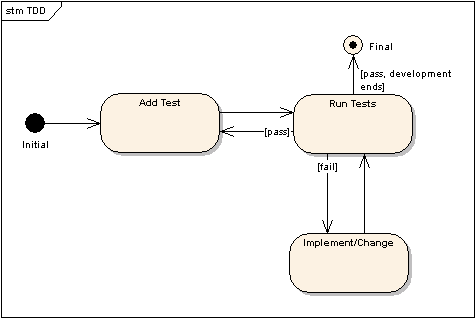
\includegraphics[scale=0.7]{graphics/TDD.png}
	\caption{Test Driven Development (TDD)}
	\label{fig:TDD}
\end{figure}

Python wird mit dem \verb|unittest| Modul\footnote{PyUnit: http://pyunit.sourceforge.net/} ausgeliefert und ist die Pythonvariante von \emph{JUnit}\footnote{JUnit: http://junit.org/}, bekannt aus der Java-Welt. Das Modul kann somit unter \Zope\ verwendet werden.

Nachfolgend ist ein einfacher Testcase mit dem \verb|unittest| Modul unter Python dargestellt:

\begin{lstlisting}[style=interpreter]
>>> import unittest
>>> class MyTestCase(unittest.TestCase):
...		def test_TwoMinusThree(self):
...			self.assertEqual(2 - 3, -1)
...			self.failIfEqual(2 - 3, 1)
...		
>>> unittest.main()
\end{lstlisting}

\paragraph*{Integration Tests und Functional Tests}

\emph{Integration tests} testen die Interaktion zwischen Komponenten, f�r die schon erfolgreich laufende \emph{Unit tests} geschrieben wurden. Dabei wird zum ersten Mal das Zusammenspiel der Komponenten in einem gemeinsamen Kontext getestet. Die n�chste Steigerung ist der Functional Test, bei dem das System als Black-Box betrachtet wird. Die Tests laufen aus der Sicht eines Benutzers.

\begin{quote}
{\itshape "'[...] in the Zope world, functional tests are really integration tests. Functional tests would treat Zope like a black box. "'Functional tests"' in Zope, however, do not simulate a browser client program and connect through the \HTTP\ port. They only simulate the necessary objects, such as the browser request. That means, they are more like integration tests."'}\cite{zope:weitershausen}
\end{quote}

Unter Zope gibt es keine Trennung der beiden Testbegriffe. Es wird unkorrekterweise einheitlich von \emph{Functional tests} gesprochen.

\paragraph*{Doctests}  

\emph{Doctesting} ist eine eigene Art Pythons, Dokumentation mit Tests zu verschmelzen. �blicherweise sind Tests selbst schon eine gute Dokumentation, wenn man die Funktionalit�t einer Komponente verstehen will. Meist sind sie aber nicht gerade komfortabel zu lesen. 

\begin{quote}
{\itshape "'Doctest is a system for writing tests within Python documentation strings.
The emphasis is on documentation. Tests are provided as example code, set
off with Python prompts. Doctest tests lend themselves toward a literate form
of test code."'}\cite{misc:pycon2004doctest}
\end{quote}

Ein \emph{Doctest} wird entweder in den \emph{Docstring}\footnote{Docstring: http://en.wikipedia.org/wiki/Docstring} im Quelltext geschrieben, oder als eigenes Textfile abgelegt. Letzteres empfiehlt sich bei umfangreicher Testl�nge. Aus den \emph{Docstrings} k�nnen seperate Dokumentationen, z.B. als \HTML\ oder \PDF\/ extrahiert werden. \emph{Doctests} werden im Stil einer Interpreter Session geschrieben. Erkl�rende Worte dazu sind im \emph{reStructuredText} Format\footnote{reStructuredText: http://docutils.sourceforge.net/rst.html} zu w�hlen. Listing \ref{python:doctest} zeigt ein kurzes Beispiel zur Veranschaulichung.

\begin{lstlisting}[style=example, caption={Doctest from the Zope 3 SessionCredentials Plugin}, label=python:doctest]
...
class SessionCredentials(object):
    """Credentials class for use with sessions.

    A session credential is created with a login and a password:

      >>> cred = SessionCredentials('scott', 'tiger')

    Logins are read using getLogin:
    
      >>> cred.getLogin()
      'scott'

    and passwords with getPassword:

      >>> cred.getPassword()
      'tiger'

    """
    def __init__(self, login, password):
        self.login = login
        self.password = password
        
    def getLogin(self): return self.login
    def getPassword(self): return self.password
...
\end{lstlisting}


\emph{Doctests} k�nnen  \emph{Unit tests} und \emph{Integration tests} in einem besser les- und schreibbaren Format abbilden.  Der Entwickler kann anhand einer "'Erz�hlung"' seinen Quelltext dokumentieren und zugleich testen. Die Vorteile liegen auf der Hand. Die Handhabung schl�gt zwei Fliegen mit einer Klappe und ist leichter zu erlernen als z.B. das \emph{Unit test} \API\/. Diese Art von Dokumentationstest erscheint dem Autor ein gutes Werkzeug, um die Thematik Testen und Dokumentieren im Unterricht darzulegen.

%Zope3 Teststrategie Zope philisophy
%Zope besteht aus xx tests..

%automatisierung
  
  \newpage	
  \subsection{Beispielimplementierung}
  \label{kapitel:Beispielimplementierung}
  	Die Beispielimplementierung behandelt einen Auszug aus einem konkreten Projekt des Autors. Das Projekt Stadtgespr�che\footnote{Stadtgespr�che: http://www.stadtgespraeche.com} ist ein digitales Museum f�r fotographische Fundst�cke von Schriften, Logos, Zeichen, Pictogrammen, Buchstaben, Wappen und anderen typografischen Werken. Der Museumsdirektor Markus Hanzer beschreibt Stadtgespr�che (Abbildung \ref{fig:stadtgespraeche}) wie folgt:

\begin{quote}
\itshape{"'Stadtgespr�che versteht sich als ein offenes Forum der Diskussion und Auseinandersetzung �ber visuelle Alltagskommunikation und versucht durch Gegen�berstellungen und analytische Beschreibungen einen Blick auf m�gliche Hintergr�nde und Motive f�r konkrete Gestaltungsformen zu werfen."'}
\end{quote}
 
Urspr�nglich wurde das Projekt im Jahre 2000 auf Basis von \Zope\ 2 unter dem Namen Typemuseum entwickelt. Aus rechtlichen Gr�nden musste das Projekt neu entwickelt werden. Zu diesem Anlass gibt es einen Technologierelaunch auf Basis von \Zope\ 3.

Die folgenden Seiten zeigen nur Ausschnitte aus den Quelltexten, in denen teilweise aufbauend erl�utert wird. Daher ist es notwendig, den tats�chlichen Endstatus der Quelltexte im Anhang dieser Arbeit abzulegen.

\begin{figure}[h]
	\centering
	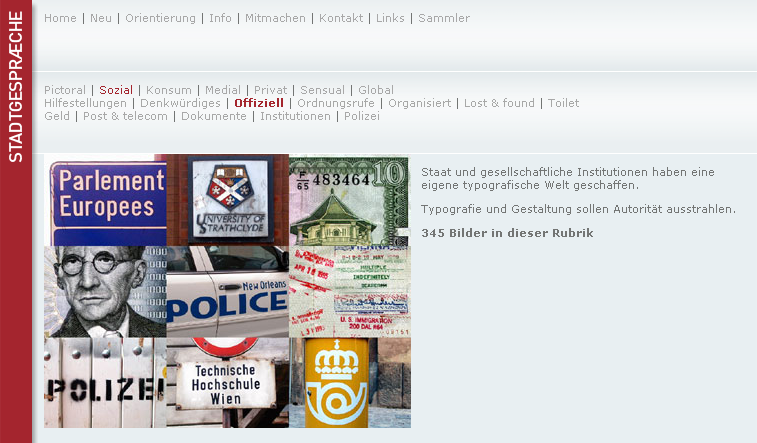
\includegraphics[scale=0.5]{graphics/stadtgespraeche.png}
	\caption{Frontend Stadtgesp�che}
	\label{fig:stadtgespraeche}
\end{figure}

Das Prinzip ist einfach. Als Gesch�ftsobjekt kann ein Eintrag im Museum definiert werden. Ein Eintrag ist eine Grafik mit zugeh�rigen Metadaten, die in einer hierarchischen Struktur abgebildet wird. Aus dieser Struktur wird die Navigation f�r das Frontend generiert.

\newpage
\subsubsection*{Interface}

\begin{figure}[h]
	\centering
	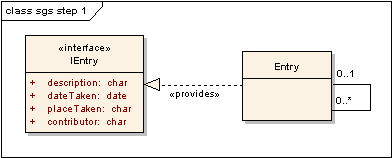
\includegraphics[scale=0.7]{graphics/sgsstep1.png}
	\caption{Interface}
	\label{fig:sgsstep1}
\end{figure}

Im ersten Schritt wird das Interface definiert. Interfaces sind kein Standardkonzept von Python und wurden von \Zope\ zus�tzlich implementiert. Aus diesem Grund sind Interfaces Klassen. Das hat wiederum den Vorteil, dass Interfaces vererbt werden k�nnen.

Interfaces unter \Zope\ 3 dienen nicht nur der Dokumentation, sondern k�nnen auch adaptiert werden. Jedes Objekt kann jedes Interface zur Verf�gung stellen oder adaptieren.

Nach Erstellen eines Python Moduls mittels leerer \verb|__init__.py| im Python Pfad (normalerweise in der Zope Instanz unter \verb|lib/python|), wird das Interface erzeugt. Nach Konvention sind die Interfaces eines Moduls immer in der Datei \verb|interfaces.py| zu finden.

\begin{lstlisting}[style=example, caption={IEntry interface (interfaces.py)}, label=impl:interface1]
from zope.app.file.interfaces import IImage
from zope.app.container.interfaces import IContainer
from zope.app.container.constraints import contains
from zope.schema import Text, TextLine, Date

class IEntry(IImage):
    """ Interface for Entry  """

    description = Text(title=u"Image Description", required=False)

    dateTaken = Date(title=u"Date when picture was taken", required=True)
    placeTaken = TextLine(title=u"Place where picture was taken",
                          required=True)

    contributor = TextLine(title=u"email of contributor", required=True)


class IEntryContainer(IContainer):
    """ Container Interface for an Entry """
    contains(IEntry)
\end{lstlisting}

\begin{itemize}
	\item Zeile 6: \verb|IEntry| erbt das \verb|IImage| Interface aus \verb|zope.app.file.interfaces|. Damit ist es m�glich, die Funktionalit�t des Zope Basis Objektes \verb|Image| zur Verf�gung zu stellen. Dieses speichert unter anderem die Bilddaten als Attribut auf dem Objekt.
	\item Zeile 7: Python Docstring f�r die Dokumentation des Interfaces.
	\item Zeile 9-15: Das Schema f�r die Attribute wird festgelegt. Ein Schema bringt eine statische Typisierung in die dynamisch typisierte Sprache Python. Hauptanwendung ist dabei das Generieren und Validieren von Userinput. Zust�ndig daf�r ist beispielsweise \verb|zope.formlib|. Sp�ter wird der Zope Server aus diesen Informationen passende Formulare generieren.
	\item Zeile 18-20: Hier ist eine andere Verwendung f�r Interfaces zu sehen. Objekte, die IEntryContainer zur Verf�gung stellen, erlauben, andere Objekte zu beinhalten, die wiederum das Interface IEntry bereitstellen. Man spricht auch von einem \emph{Marker-Interface}.
\end{itemize}

\subsubsection*{Content Objekt}

Im n�chsten Schritt legen wir ein Content Objekt an, das obige Interfaces implementieren wird.

\begin{lstlisting}[style=example, caption={persistentes Content Objekt (entry.py)}, label=impl:content1]
from zope.interface import implements
from zope.app.container.btree import BTreeContainer
from zope.app.file.image import Image

from interfaces import *

class Entry(BTreeContainer, Image):
    implements(IEntry, IEntryContainer)

    __name__ = __parent__ = None

    description = u""

    dateTaken = None
    placeTaken = u""

    contributor = u""
\end{lstlisting}
\begin{itemize}
	\item Zeile 7: Unsere Klasse erbt die Funktionalit�t von \verb|Image| und \verb|BTreeContainer| und damit implizit auch eine automatische Persistierung in der \ZODB\/. \verb|BTreeContainer| erm�glicht, weitere Objekte \emph{in} einer \verb|Entry| Instanz zu speichern. Die Klasse fungiert somit als Container. Die enthaltenen Objekte werden aus Performancegr�nden als Binary Tree abgelegt.
	\item Zeile 8: Das Objekt implementiert hiermit die beiden von uns erstellten Interfaces. Somit ist es m�glich, das Content Objekt ineinander zu verschachteln.
	\item Zeile 10: Diese beiden Attribute werden ben�tigt, um das Objekt in der Hierarchie auffindbar zu machen (\verb|zope.location|).
	\item Zeile 12-17: Um die Anforderungen der Interfaces zu erf�llen, werden die im Interface definierten Attribute leer initialisiert.
\end{itemize}

\subsubsection*{Konfiguration}

Per \ZCML\ wird dem \Zope\ Server nun mitgeteilt, dass die neue Komponente bereit ist, in Betrieb genommen zu werden.

\begin{lstlisting}[style=example, caption={ZCML Konfiguration (configure.zcml)}, label=impl:zcml1]
<configure
        xmlns="http://namespaces.zope.org/zope"
        i18n_domain="zope"
        >

<class class=".entry.Entry" >
    <require
        permission="zope.View"
        interface=".interfaces.IEntry" />
    <require
        permission="zope.View"
        interface=".interfaces.IEntryContainer" />
    <require
        permission="zope.ManageContent"
        set_schema=".interfaces.IEntry" />
</class>

</configure>
\end{lstlisting}

\begin{itemize}
	\item Zeile 6-16: Der \verb|class| Tag registriert und konfiguriert das Objekt innerhalb von Zope. Standardm��ig ist der Zugriff auf alle Elemente einer Klasse von der Zope Security Maschinerie unterbunden. In diesen Zeilen wird der Lesezugriff auf alle durch die Interfaces \verb|IEntry| und \verb|IEntryContainer| definierten Attribute f�r die Zope Permission \verb|zope.View| freigegeben. Der Schreibzugriff wird f�r das Schema unter \verb|IEntry| zugelassen.
\end{itemize}

Um das Objekt per \ZMI\ verwalten zu k�nnen, erstellen wir eine eigene Konfiguration im Untermodul \verb|browser|. Das signalisiert die Zugeh�rigkeit zu einem View der \HTTP\ Klasse. Daf�r wird das Unterverzeichnis erstellt und als Python Modul gekennzeichnet. In die obige Datei \verb|configure.zcml| wird das neu zu ber�cksichtigende Modul wie folgt eingef�gt.

\verb|<include package=".browser" />|

Das \verb|browser| Modul wird in Zukunft alle Views betreffend Webbrowser enthalten.

\begin{lstlisting}[style=example, caption={ZCML Browser Konfiguration (browser/configure.zcml)}, label=impl:zcml1]
<configure xmlns="http://namespaces.zope.org/browser">

<addMenuItem
      class="..entry.Entry"
      title="SGS Entry"
      permission="zope.ManageContent"
      view="AddSGSEntry.html"
      />

<addform
      label="Add SGS Entry"
      name="AddSGSEntry.html"
      schema="..interfaces.IEntry"
      content_factory="..entry.Entry"
      class="zope.app.file.browser.image.ImageAdd"
      permission="zope.ManageContent"
      />

<containerViews
      for="..interfaces.IEntryContainer"
      contents="zope.ManageContent"
      add="zope.ManageContent"
      />
      
</configure>
\end{lstlisting}

Diese Konfiguration erm�glicht dem Administrator nun via \ZMI\ neue Instanzen des \verb|entry| Content Objektes zu erstellen (siehe Abbildung \ref{fig:zmi1}). Die daf�r ben�tigten Webformulare, inklusive Validierung, wurden durch die vorherigen Interfacespezifikationen erstellt.

\begin{figure}[ht]
	\centering
	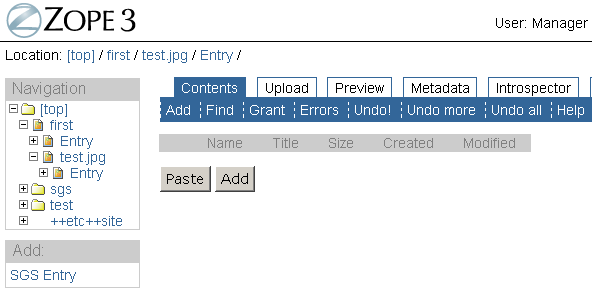
\includegraphics[scale=0.5]{graphics/zmi1.png}
	\caption{Zope Management Interface (ZMI)}
	\label{fig:zmi1}
\end{figure}

%TODO eventuell Schema (email)

\subsubsection*{Adapter}

Die Persistierung und Konfiguration eines Eintrages ist erledigt. Nun wird dieser um die Funktionalit�t einer Navigation erweitert. Dabei wird darauf geachtet, dass browser-spezifische Funktionalit�t abgekapselt, und weiters die bisherige Implementierung nicht ge�ndert wird. Dabei kommt ein Werkzeug des Zope Komponenten Frameworks zum Einsatz: der Adapter.

Mittels Adapter kann die bestehende Funktionali�t erweitert werden, ohne die Implementierung des zu adaptierenden Objektes zu �ndern.

Die Datei \verb|interfaces.py| wird um das Interface des Adapters erweitert.

\begin{lstlisting}[style=example, caption={Adapter Interface f�r Navigationsfunktionalit�t (interfaces.py)}, label=impl:adapterinterface, firstnumber=22]
from zope.interface import Interface

class IEntryNav(Interface):
    """used as Adapter for menu creation
    """

    def setEntryMenuName(menuname):
        """ set the navigation menu name  """

    def getEntryMenuName():
        """ get the navigation menu name """

    def getEntryMenuOrder():
        """ get the navigation menu order """

    def setEntryMenuOrder(order):
        """ set the navigation menu order """

    def getChildren():
        """ get all IEntry children from this location """

    def getSiblings():
        """ get all IEntry Siblings from this location
            (self is included)
        """
\end{lstlisting}

\begin{figure}[h]
	\centering
	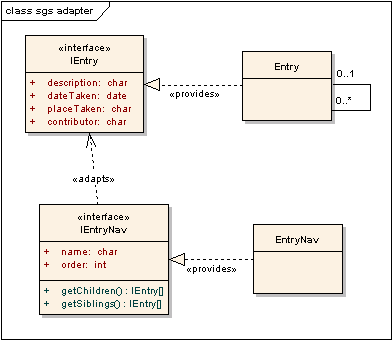
\includegraphics[scale=0.7]{graphics/sgsadapter.png}
	\caption{Adapter}
	\label{fig:sgsadapter}
\end{figure}

\verb|Entry| soll um ein Attribut erweitert werden, das den Namen des Navigationspunktes repr�sentiert. Weiters soll jeder Men�punkt eine Gewichtung zwecks Sortierung der Navigation erhalten. Der Name des Navigationspunktes wird als \emph{Annotation} auf dem urspr�nglichen Objekt gespeichert. Dazu muss \verb|Entry| ein Markerinterface zur Verf�gung stellen, welches signalisiert, dass auf diesem Objekt Metadaten (Annotations) gespeichert werden d�rfen. Das kann entweder via \ZCML\ oder wie folgt (Listing \ref{impl:changeentry}) geschehen. 

\begin{lstlisting}[style=example, caption={Hinzuf�gen des Marker Interfaces f�r Annotations (entry.py)},firstnumber=8, label=impl:changeentry]
implements(IEntry, IEntryContainer, IAttributeAnnotatable)
\end{lstlisting}

\begin{lstlisting}[style=example, caption={Adapter f�r Navigationsfunktionalit�t (entry.py)}, label=impl:adapter, firstnumber=19]
from zope.component import adapts
from zope.annotation.interfaces import IAttributeAnnotatable
from zope.annotation import IAnnotations

EntryNavAnnotations_KEY = "sgs.entrynav"

class EntryNav(object):
    implements(IEntryNav)
    adapts(IEntry)

    def __init__(self, context):
        self.context = self.__parent__  = context
        annotations = IAnnotations(context)
        mapping = annotations.get(EntryNavAnnotations_KEY)
        if mapping is None:
             mapping = annotations[EntryNavAnnotations_KEY] = {'name': '',
                                                              'order': 0}
        self.mapping = mapping

    def setEntryMenuName(self, menuname):
        self.mapping['name'] = menuname

    def getEntryMenuName(self):
        return self.mapping['name']

    def setEntryMenuOrder(self, order):
        self.mapping['order'] = order

    def getEntryMenuOrder(self):
        return self.mapping['order']

    def getChildren(self):
        return self.context.values() 

    def getSiblings(self):
		siblings = []
        for sibling in self.context.__parent__.values():
            if IEntry.providedBy(sibling):
                siblings.append(sibling)
        return siblings
\end{lstlisting}

\begin{itemize}
	\item Zeile 26: Diese Klasse stellt \verb|IEntryNav| als Interface zur Verf�gung,
	\item Zeile 27: und fungiert als Adapter f�r IEntry (siehe Abbildung \ref{fig:sgsadapter}).
	\item Zeile 30-36: Um die beiden neuen Attribute zu persistieren, wird der IAnnotations Adapter auf dem \verb|Entry| Objekt angewendet.
	\item Zeile 38-48: getter und setter der neuen Attribute.
	\item Zeile 50-58: Implementierung der Methoden, die die sp�tere Navigationsgenerierung unterst�tzen.
\end{itemize}
	
Um den Adapter zu registrieren, muss der Konfigurationsteil im \verb|entry| Modul erweitert werden (Listing \ref{impl:adapterzcml}).

\begin{lstlisting}[style=example, caption={ZCML Konfiguration f�r den Adapter der Navigationsfunktionalit�t (configure.zcml)}, label=impl:adapterzcml, numbers=none]
...
<adapter factory=".entry.EntryNav"
         trusted="true"  />

<class class=".entry.EntryNav" >
    <require
        permission="zope.View"
        interface=".interfaces.IEntryNav" />
</class>
...
\end{lstlisting}

Ein Test f�r die Adapterimplementierung ist �berf�llig. Listing \ref{anhang:entry.txt} aus dem Anhang erl�utert diesen.

Als N�chstes wird ein Browser-View geschrieben, der die Navigation nach Abbildung \ref{fig:stadtgespraeche} generiert. Der View kann in Folge von einem \ZPT\ verwendet werden, um diesen f�r den Benutzer graphisch aufzubereiten.

\lstinputlisting[style=example, caption={Generierung der Navigation (browser/\_\_init\_\_.py)}]{code/browser/__init__.py}

\begin{itemize}
	\item Zeile 13-21: Das soeben aktive Objekt sucht seine Elternobjekte in der Hierarchie und ordnet diese in eine Liste ein.
	\item Zeile 23-29: F�r jeden Eintrag in der soeben generierten Liste steht ein aktiver Men�punkt in der Navigation. F�r jeden dieser Men�punkt werden die Geschwistereintr�ge auf gleicher Ebene gesucht. Die Information wird als Liste von Dictionaries generiert. Gleichzeitig wird die Navigation korrekt sortiert.
	\item Zeile 31-45: Der gleiche Vorgang wie zuvor findet f�r die Eintr�ge auf gleicher Ebene und die Kinder des aktiven Objektes statt.
\end{itemize}

Im Anhang ist der komplette Quelltext der Beispielimplementierung zu finden, sowie weitere Tests, die die Generierung der Navigation und eine Katatalogindizierung testen.

Weitere Schritte in der Implementierung betreffen sowohl die Pr�sentationslogik, als auch das Layout mit \HTML\ und \CSS\/ sowie ein Redakteursinterface. Das wird in dieser Arbeit nicht behandelt. M�gliche weitere denkbare Funktionalit�ten w�ren eine Tagging Engine, mit der es m�glich ist, Eintr�ge zu verschlagworten und somit eine flache Kategorisierung zu erreichen (im Gegensatz zur Hierarchie der momentanen Implementierung). Ein fertige Komponente hierf�r scheint \verb|lovely.tag|\footnote{lovely.tag: http://svn.zope.org/lovely.tag/} zu sein. 

%TODO eventuell DANN security, pluggable auth


%Abhandlung der Implementierung. Systematisches Vorstellen des Frameworks anhand der Implementierung. Optimalerweise k�nnte das ein Beispielprojekt f�r Unterrichtszwecke sein.
%Genaues Thema der Implementierung steht noch nicht fest. Fokus liegt auf der Implementierung, nicht auf auf Analyse oder Design.
%Der Aufbau soll sich an \cite{zope:weitershausen} anlehnen.
  
%Die folgende Unterteilung in Unterkapitel ist implementierungsbedingt und wird sich mit gro�er Wahrscheinlichkeit noch anpassen. Sie ist als einstweiliges Grundkonzept zu sehen.
%  	\subsubsection{Interfaces}
%  	\subsubsection{Content Components}
%  	\subsubsection{Views}
%  	\subsubsection{Internationalization}
%  	\subsubsection{Adapters}
%  	\subsubsection{Automatisches Testen}
%  	\subsubsection{Metadaten und der Dublic Core Standard}
%  	\subsubsection{Sicherheit}
%  	\subsubsection{Authentifizierung und Benutzerverwaltung}
  	
  \subsection{Die Zukunft von Zope}
  \label{kapitel:zukunftzope}
  \Zope\ ist und war ein innovativer Vorreiter bei Webtechnologien. In der Implementierung von Web-applikationen liegt die gro�e St�rke des Frameworks. Gleichzeitig ist durch die einfache Handhabung ein leichter Zugang in die Materie m�glich. Die Barrieren bei L�sungen aus der Java-Welt sind durchaus h�her. Somit kann eine Verwendung in der Lehre erwogen werden.\cite{zope:futurefaasen}

Ein aktuelles Projekt der \Zope\ Community ist \emph{Grok}\footnote{Grok: http://grok.zope.org/}. Grok ist ein Ansatz, den Zugang zur \Zope\ Komponentenarchitektur weiter zu vereinfachen. Momentan ist das Projekt in Entwicklung und sollte weiter beobachtet werden.

\begin{quote}
{\itshape "'I hope with Grok we will have drastically increased the approachability of Zope 3. This will hopefully make it the web framework of choice for more web developers (Python), even given the intense competition. I also hope that Zope 3 will continue to adopt technologies from outside the Zope realm, sharing code and concepts with other Python-based web frameworks. At the same time, Zope 3's components will become more separate from a monolithic application server and will start to be reused more within other web frameworks [...] Zope 2 applications will continue to evolve using Five towards using Zope 3 technology. The platforms Zope 2 and Zope 3 will continue to merge."'}\cite{zope:futurefaasen}
\end{quote}
  
\Zope\/, vor allem \Zope\ 3, ist jedoch nur einem kleinen Teil der Entscheidungstr�ger bekannt. Das sollte ein Hauptaugenmerk der Zope Community in naher Zukunft sein. Beispielsweise ist die Zope Website schwer vernachl�ssigt, was bestimmt ein Grund ist, warum so mancher Interessierte scheitert. Das Framework und dessen M�glichkeiten, vor allem auch Erfolgsgeschichten sollten besser an die �ffentlichkeit kommuniziert werden. Einen Beitrag dazu soll diese Arbeit leisten.
  
  
	\subsection{Alternative Python Frameworks}
	%Vorstellen anderer Python-Webframeworks (Django, Turbogears). Sehr allgemein gehalten.
%Pylons, Pocoo and Clever Harold? (siehe http://www.sqlalchemy.org/)

Es existieren diverse alternative Python Frameworks, die oft in einem Zug mit \Zope\ 3 erw�hnt werden. Dabei muss beachtet werden, dass diese Frameworks eher auf spezielle Bed�rfnisse im Web zugeschnitten sind und mehr Frontend- als Backendentwicklung unterst�tzen. Es scheint, dass die meisten dieser Frameworks auf den Web2.0-Hype aufspringen und sich dabei auf die Erstellung von Wiki, Weblog, Forum, \emph{\RSS\/} und ein \emph{\AJAX\/} gesteuertes Userinterface spezialisieren. Die folgenden Frameworks basieren alle auf Python und werden mit Objektmapper-Funktionalit�t (siehe Kapitel \ref{sec:ZODB}) zur Verf�gung gestellt.

\begin{itemize}
	\item Turbogears\footnote{Turbogears: http://www.turbogears.org/}
	\item Django\footnote{Django: http://www.djangoproject.com/}
	\item Pylons\footnote{Pylons: http://pylonshq.com/}
\end{itemize}

Allerding ist \Zope\ 3 nach Ansicht des Autors das geeignete Tool, um anhand interessanter und einfacher Applikationsentwicklung, notwendige Thematik  verst�ndlich in den Unterricht zu integrieren. Diese Themen sind Testen von Software, kollaboratives Arbeiten, wissenschaftliches Arbeiten (Nachvollziehbarkeit ist auch in der Softwareentwicklung notwendig!), Komponentenverst�ndnis und Wiederverwendbarkeit, die ihren Einzug in die Lehre vor allem in praktischer Hinsicht noch nicht gefunden haben! Obig angef�hrte Frameworks scheinen jedoch f�r einfache Webapplikationsprojekte einen einfacheren Zugang zu bieten.

  

\newpage
\section{Diskussion}
\rkopf[]{Diskussion}	
	\subsection{Zusammenfassung und Bewertung}
		%.) einleitende Bemerkung
In der vorliegenden Arbeit wurde die Eignung Pythons als Werkzeug f�r den Einsatz im Unterricht analysiert. Beweggr�nde f�r das Schreiben der Arbeit waren die positiven Erfahrungen des Autors mit Python in seinem Arbeitsumfeld und Beobachtungen w�hrend seines Studiums an der \FH\ Technikum Wien, wo mit C und Java unterrichtet wird. Der Autor wollte untersuchen, ob und wie sich Python f�r den Einstieg in die Programmierung als auch f�r fortgeschrittene Softwareentwicklung, eignet. Beim Thema Softwareentwicklung lag das Augenmerk auf dem Applikationsserver \Zope\/\footnote{Im Folgenden wird immer von Zope ab der Version 3 gesprochen. Ist die Rede von einer fr�heren Version, wird explizit die Versionsnummer angef�hrt.}.

%.) r�ckblick zur Einleitung
In der Einleitung wurde mit der Vorstellung der fundamentalen Idee einer Wissenschaft, die, nach Ansicht des Autors, gerade in der informatischen Bildung, im Zusammenhang mit Programmiersprachen, nicht ber�cksichtigt wird, begonnen. Durch die Komplexit�t der Programmiersprachen verliert sich der Unterricht in Details einer Sprache oder eines Tools. Die zu vermittelnden fundamentalen Ideen kommen dabei zu kurz. Danach wurde ein kurzer �berblick �ber die Probleme beim Erlernen einer Programmiersprache gegeben. Python und Zope wurden im Anschluss vorgestellt. Dabei ist der Autor auf die Geschichte und die Unterschiede zwischen den Versionen (vor allem zwischen Zope 2 und Zope 3) eingegangen.

%.)python
%..)R�ckblick
Das erste Kapitel hat sich mit Python besch�ftigt. Vor allem der Einsatz von Python als erste Programmiersprache wurde anhand eines Vergleichs mit C++ und Java illustriert. Dabei wurde anhand des banalen \emph{Hello World} Beispiels\footnote{Das traditionelle erste Programm eines jeden angehenden Softwareentwicklers.} erl�utert, wo die didaktischen Schwachstellen liegen, wenn eine Systemsprache als erste Programmiersprache gew�hlt wird. Hierbei wurde davon ausgegangen, dass Studenten wenig bis keine Programmiererfahrung haben. Im weiteren Verlauf des Kapitels setzte sich die Arbeit mit Programmierparadigmen und Algorithmen auseinander, um herauszustreichen, welche Vorteile Python hier f�r sich verbuchen kann. Auch der Aspekt von Open-Source und deren Community wurde in Hinblick auf deren m�glichen positiven Einfluss auf den Unterricht beleuchtet. Das Kapitel wurde mit der Vorstellung diverser Materialien und Werkzeuge, die f�r die Gestaltung des Unterrichts mit Python herangezogen werden k�nnen, beendet.

%..)Ergebnis
Dabei wird offenbar, dass der Einsatz von Systemsprachen f�r das Lehren von Programmieraspekten nicht besonders geeignet ist. Um ein einfaches Programm zu schreiben, sind zu komplexe und fortgeschrittene Zusammenh�nge zu durchschauen, die den Studenten schwer im Vorfeld beizubringen sind. Das Ergebnis sind frustrierte und desinteressierte, potentielle Softwareentwickler. Ziel des Informatikunterrichts sollte es sein, zu begeistern. Daf�r ist es notwendig, den Studenten schnelle Erfolge zu erm�glichen. Das Kapitel zeigt, dass dieses Ziel mit Python, aufgrund des Aufbaus der Sprache an sich,  einfacher zu erreichen ist. Auch die Seite des Unterrichtenden wurde analysiert. Dabei ist festgestellt worden, dass f�r die Gestaltung eines Curriculums mit Python gen�gend bestehendes Material vorhanden ist, an dem sich orientiert werden kann. Die Wahl einer Skriptsprache wie Python erleichtert Studenten wie Lektoren die Arbeit und erm�glicht, den Unterricht auf die fundamentalen Ideen der Informatik zu konzentrieren.

Es wird festgestellt, dass die Entscheidung, Sprachen wie C, C++ oder Java im Unterricht zu verwenden, stark industriegetrieben ist, was durch das Fehlen einer allgemein anerkannten Lehrsprache, wie es Pascal fr�her einmal war,  noch verst�rkt wird. Studenten neigen auch dazu, sich eher f�r Programmiersprachen zu interessieren, die sie in ihrem sp�teren Berufsleben verwenden k�nnen. Diese beiden Motivationen ergeben die momentane Situation in der Lehre.

%..)Konsequenzen
F�r die Zukunft ist es w�nschenswert, dass erkannt wird, dass nicht das Wissen um eine spezielle Programmiersprache wichtig ist, sondern das Erlernen der grundlegenden Konzepte. Sind diese erst einmal verstanden, k�nnen sie mit jeder Programmiersprache umgesetzt werden. Daf�r ist Python aus der Sicht des Autors bestens geeignet. Als Unterstreichung dieser Aussage soll das folgende Zitat von Eric Steven Raymond\footnote{http://en.wikipedia.org/wiki/Eric\_Steven\_Raymond} dienen.

\begin{quote}
{\itshape "'Python is, of all the languages I have learned, the one that does the least to get between me and the problem. It�s the most effective to translate pure thoughts into action."'}
\end{quote}

Doch ist Python auch au�erhalb der Lehre sinnvoll anzuwenden? Der aufmerksame Leser hat festgestellt, dass verstandene Konzepte aus der Lehre auf alle Anforderungen au�erhalb der Lehre angewendet werden k�nnen. Diese sind unabh�ngig von Programmiersprachen. Aber Menschen in eingefahrenen Systemen geh�ren wachger�ttelt. Diese Arbeit verweist auf den erfolgreichen Einsatz von Python in der Softwareindustrie.

%.)Zope
%..)R�ckblick
Im zweiten Hauptkapitel wurde das Lehren von fortgeschrittenen Themen der Softwareentwicklung mit Hilfe des Applikationsservers \Zope\/ thematisiert. \Zope\ wurde in der Einleitung als Komponentenframework vorgestellt. Damit hat sich dieses Kapitel zu Beginn auseinandergesetzt. Danach wurde versucht, \Zope\ mit dem \CBSE\ in Verbindung zu bringen und einzuordnen. Anschlie�end wurde die \ZODB\ und deren m�glicher Einsatz in der Lehre vorgestellt. Das Entwickeln einer Software ist ein komplexer Prozess und schwierig im Unterricht zu vermittelt. Damit hat sich ein Teil dieses Kapitels besch�ftigt, ebenso wie mit dem stark vernachl�ssigten Testen und Dokumentieren von Software.

%..)Ergebnis
Die Arbeit stellt fest, dass auch fortgeschrittene Themen in der Softwareentwicklung mit Python behandelt werden k�nnen. \Zope\ wurde mit Python entwickelt und steht selbst als Beispiel f�r den erfolgreichen Einsatz Python�s in der Industrie. \Zope\ hat seinen Fokus auf Webapplikationen, ist dabei aber nicht auf diesen Einsatz beschr�nkt. Der Autor meint, dass der Einsatz von \Zope\ einen einfachen Zugang f�r die Entwicklung von komplexeren Applikationen im universit�ren Einsatz erm�glicht. Dabei kann der Fokus auf Reuse, komponentenorientieres Denken und Testen bzw. Dokumentieren von Software gelegt werden. 

%..)Konsequenzen
Berichte vom Einsatz von \Zope\ \emph{in} der Lehre gibt es keine. \Zope\ wird eher \emph{f�r} die Lehre verwendet. Als Beispiel sei die \MUW\  genannt, wo momentan die zentrale Pr�fungsverwaltung mit \Zope\ und Python entwickelt wird. Aufgrund der fehlenden Erfahrung im Umgang mit \Zope\ innerhalb eines Curriculums, sollten Versuche gestartet werden, um festzustellen, ob sich \Zope\ dabei bew�hren kann. Die Zeit ist reif f�r einen Versuch, wenngleich der momentane komplexe Einstieg in die Komponentenarchitektur von \Zope\ eventuell in einer Schulung zum Framwork selbst enden k�nnte. Die H�rde, das Komponentenframework zu verstehen und anzuwenden, ist momentan noch etwas zu hoch. Daran wird aber gearbeitet. Die \Zope\ Community bem�ht sich zur Zeit um ein Projekt namens \emph{Grok} (siehe Kapitel \ref{kapitel:zukunftzope}), das die hohe Anfangsbarriere senken m�chte.


%.)Abschlie0ender Kommentar (mit abschlie�ende Zitate)
%TODO?




%Der Inhalt dieses Kapitel wird sich erst im Laufe der Arbeit ergeben.
%{\color{red} tr�gheit der lehre.  industrie-> lehre 10 jahre UML seit 1995, VORSICHT, teilweise schon eingearbeitet (paradigmen)}
%	Industrialisierung der Softwareindustrie; umsomehr ist es wichtig, nur die fumdamentalen Konzepte zu erl�utern. ev sind sp�ter einmal nicht mehr so viele Programmierexperten notwendig.
	
%Die im Kapitel Python-Open Source und COmmunity erw�hnte ansatz der kanalisierten newsgroup bzw kommunikationsplatformen??
	

	%passt vielleicht besser zu python first kapitel als abschluss?
%\emph{ I think this language, above just about all others at the time of this writing, is accessible enough to not get in the way, not consume too many brain cycles, even as we're trying to get through quite a lot of material. It will become the student's friend, less his frustrating foe, helping her or him to gain insights into the material, versus obfuscating it with a lot of clutter and extraneous syntax.}\cite{python:math}
	
%zusammenfassung zope, komplex. GROK, interview matijn faasen
		
	\subsection{Kritik}
		Nachfolgende Aufstellung stellt eine zusammenfassende Liste der Argumentation dar, wobei die jeweiligen Alleinstellungsmerkmale fett hervorgehoben sind. Diese werden den negativen Kritikpunkten gegen�bergestellt. Dabei ist zu beachten, dass diese Aufstellung nicht alle Vor- und Nachteile von Python und Zope, sondern bewusst die der vorgestellten L�sung, Python und Zope als Unterrichtswerkzeuge, zeigt.

%kritische bewertung der vorgestellten l�sung:
%welche Nachteile gibt es
%wo liegen die grenzen, etc

\newenvironment{vorteile}{
  \renewcommand{\labelitemi}{$+$}
}

\newenvironment{nachteile}{
  \renewcommand{\labelitemi}{$-$}
}

Python:
\begin{vorteile}
\begin{itemize}
\item \textbf{Multiparadigmensprache}
\item \textbf{erzwungene Einr�ckung des Quelltextes}
\item einfacher Zugang zur Programmierung m�glich
\item einfache Installation
\item einfache Entwicklungsumgebung
\item Python kann als Werkzeug im Unterricht verwendet werden und wird nicht Gegenstand des Unterrichts selbst
\item der Untericht kann sich auf die fundamentalen Ideen des zu vermittelnden Wissens konzentrieren
\item schnelle Lehr- und Lernerfolge
\item Erleichterung bei der Gestaltung von Curricula
\item auch f�r junge Zielgruppe geeignet (Unterstufe)
\item gute Vorbereitung auf komplexere Sprachen
\item gro�e Standardbibliothek
\item dynamische Typisierung
\item Open-Source Produkt
\item interpretierte Sprache
\end{itemize}
\end{vorteile}

\begin{nachteile}
\begin{itemize}
\item langsamer als Systemsprachen
\item kein Compiler
\item keine Pointer, Typisierung und Speicherverwaltung 
\item keine Systemsprache
\item Geheimnisprinzip bei der \OOP\ nicht explizit in der Sprache integriert
\end{itemize}
\end{nachteile}

\newpage
Zope:
\begin{vorteile}
\begin{itemize}
\item \textbf{objektorientierte Persistenzl�sung - \ZODB\/}
\item Komponentenframework auf Open-Source Basis
\item im Vergleich zu �hnlichen Frameworks einfacher Zugang zu komplexen Themen der Softwareentwicklung
\item m�gliches Werkzeug f�r das Vermitteln eines Softwareentwicklungsprozesses im Unterricht
\end{itemize}
\end{vorteile}

\begin{nachteile}
\begin{itemize}
\item Einstieg in die Komponentenarchitektur noch zu schwierig (vgl. Grok in \ref{kapitel:zukunftzope})
\item im Untericht noch nicht erprobt
\end{itemize}
\end{nachteile}
	
	\subsection{N�chste Schritte}
		Gregor Lingl bietet in �sterreich die Lehrerfortbildung f�r Python an. Um den Sch�lern Kosten f�r sein Buch \cite{python:forkids} zu ersparen, m�sste es approbiert werden. Weiters k�nnten mehr Angebote in der Lehrerfortbildung organisiert werden. Kurt Winterstein, ein Lehrer an einer �sterreichischen Schule meint:

\begin{quote}
{\itshape "'Langfristig m�ssten die LehrerInnen, die sich fortbilden m�chten, mehr entlastet werden. Das gilt ganz
allgemein f�r die LehrerInnenfortbildung, weil der Schulalltag meinem Empfinden nach viel
stressiger geworden ist und die Mu�e f�r eine Fortbildung fehlt."'}\cite{python:interview1}
\end{quote}

An Universit�ten und Fachhochschulen muss gepr�ft werden, ob Lehrpl�ne angepasst werden k�nnen. Als erster Schritt sollte ein Studiengang gew�hlt werden, wo das einfacher m�glich ist. Beispielsweise ein Studiengang, wo das Programmieren ein allgemeinbildendes Fach ist, von dem wenig andere Lehrveranstaltungen abh�ngen. Gleichzeitig muss �berzeugungsarbeit geleistet werden, um Python als gute Einstiegssprache und weiterf�hrende Sprache f�r fortgeschrittene Themen in der Ausbildung vorzustellen. Vorliegende Arbeit kann als Anhaltspunkt dazu verwendet werden.

Bei \Zope\ gestaltet sich ein Versuch einfacher. Hier kann eine Projektarbeit ins Leben gerufen werden. Theoretische Teile k�nnen leicht in �berblicksveranstaltungen einflie�en. Erkenntnisse daraus sollten analysiert und �ffentlich gemacht werden, da es noch keine wissenschaftliche Arbeit zum Thema "'\Zope\ im Unterricht"' gibt.

Die Entwicklung von \emph{Grok} (siehe Kapitel \ref{kapitel:zukunftzope}) sollte beobachtet werden, um  zu erfahren, ob \emph{Grok} den Zugang, zum momentan doch komplexen Einstieg in die Komponentenarchitetur von \Zope\/, erleichtert.

Langfristig k�nnte eine softwaretechnische Ausbildung mit Python und \Zope\ alle wichtigen Konzepte der Softwareentwicklung abdecken.



%{\color{red} roadmap laut letzten G�schka meeting, todos kurz-mittel und langfristig}
	
	\subsection{�hnliche Arbeiten}
		%Verweis, Zusammenfassung und Abgrenzung �hnlicher Arbeiten.
	
\cite{python:linkweiler} stellt die Frage: Eignet sich die Skriptsprache Python f�r schnelle Entwicklungen
im Softwareentwicklungsprozess? Dabei analysiert er Python in Syntax und Semantik und zeigt Parallelen zwischen den Anforderungen an Programmiersprachen zur schnellen Softwareentwicklung, und den Anforderungen aus fachdidaktischer Sicht. Seine Arbeit kann die eing�ngliche Frage positiv beantworten. Durch die Parallelen kommt er zu dem Schluss, dass Python f�r den Einsatz in der informatischen Bildung gut geeignet ist.
	
\cite{python:miller} erl�utert in seiner Arbeit, dass informatische Bildung, vor allem das Programmieren an sich, in Zukunft den gleichen didaktischen Wert wie "'herk�mmliches"' Lesen und Schreiben haben wird. Er beschreibt, wie so ein Unterricht aussehen kann und streicht dabei Python als pr�ferierte Sprache f�r diesen Einsatz hervor. Inspiriert wurde die Arbeit dabei von \cite{python:vanrossum}.

\cite{misc:diplinformatikat} widmet sich dem Unterrichtsfach Informatik und zeigt, wie schwer es ist, dieses Fach aufgrund der Schnelllebigkeit der Materie zu lehren. Die Arbeit untersucht den Informatikunterricht an �sterreichs Schulen im Jahr 2006. Gleichzeitig wird herausgearbeitet, wie sich Informatik von anderen Unterrichtsgegenst�nden grunds�tzlich unterscheidet.

\cite{misc:Modrow} besch�ftigt sich in seiner Arbeit mit Didaktikans�tzen in der informatischen Lehre. Er diskutiert dabei ausf�hrlich die in der vorliegenden Arbeit verwendete "'fundamentale Idee"' nach \cite{schwill1}.	

\cite{zope:reportcurriculum} zeigt, wie der Applikationsserver \Zope\ im Unterricht eingesetzt werden kann. Dabei wird allerdings Version 2 des Frameworks eingesetzt. Der Bericht zeigt den erfolgreichen Einsatz von \Zope\ innerhalb eines Webapplikationsentwicklungs-Curriculums.

%NAJA:	
%ev noch diss_gebrauchstaugliche_didaktische_Software.pdf
%und Einfuehrung_in_die Didaktik_der_Informatik.pdf

%%%

\newpage
%\section*{Literaturverzeichnis}
\rkopf[]{Literatur}
\bibliography{literatur}

\newpage
\rkopf[]{Abbildungsverzeichnis und Tabellenverzeichnis}
\listoffigures
\listoftables
\lstlistoflistings % code listings

\newpage
\section*{Anhang}
\rkopf[]{Anhang}
\begin{appendix}
	\section{Quelltexte}

Alle Quelltexte zu dieser Arbeit und der Status des Projektes Stadtgespr�che, sind unter \url{http://www.stadtgespraeche.com/technik} bzw. \url{http://www.mira4.com/stadtgespraeche} zu finden.

\subsection*{interfaces.py}
\lstinputlisting[style=example, caption={interfaces.py}]{code/interfaces.py}

\subsection*{entry.py}
\lstinputlisting[style=example, caption={entry.py}]{code/entry.py}

\subsection*{entry.txt}
\lstinputlisting[style=example, caption={entry.txt}, label=anhang:entry.txt]{code/entry.txt}

\subsection*{configure.zcml}
\lstinputlisting[style=example, caption={configure.zcml}]{code/configure.zcml}

\subsection*{tests/test\_entryNav.py}
\lstinputlisting[style=example, caption={tests/test\_entryNav.py}]{code/tests/test_entryNav.py}

\subsection*{browser/\_\_init\_\_.py}
\lstinputlisting[style=example, caption={browser/\_\_init\_\_.py}]{code/browser/__init__.py}

\subsection*{browser/configure.zcml}
\lstinputlisting[style=example, caption={browser/configure.zcml}]{code/browser/configure.zcml}

\subsection*{browser/tests.py}
\lstinputlisting[style=example, caption={browser/tests.py}]{code/browser/tests.py}

\subsection*{browser/catalog.txt}
\lstinputlisting[style=example, caption={browser/catalog.txt}]{code/browser/catalog.txt}  
\end{appendix}


\end{document}